\documentclass[dissertation, copyright, final, numsections, gsmodern]{uothesis}
%\documentclass[dissertation, copyright, draftcopy]{uothesis}
%\usepackage[english,UKenglish]{babel}
\usepackage[UKenglish]{babel}
\usepackage{amsmath, latexsym, amssymb}
\usepackage{natbib}
\usepackage{etoolbox}
\usepackage{mathrsfs}

\newcommand{\rednote}[1]{{\color{red} (#1)}}
\newcommand{\todoin}[1][]{\todo[inline,#1]}

%%%PREFATORY PAGES
\covertitle{Astrophysics with Gravitational Wave Signals from Core-Collapse Supernovae}
\abstracttitle{Astrophysics with Gravitational Wave Signals from Core-Collapse Supernovae}
\author{Vincent Roma}
\department{Department of Physics}
\narrowdepartment{Department Of Physics}
\degreetype{Doctor of Philosophy}
\degreemonth{June}
\degreeyear{2019}
\advisor{Ray Frey}
\chair{James Brau}
\committee{Robert Schofield & Core Member \\
Michael Kellman & Institutional Representative \\}
\graddean{Kimberly Andrews Espy}
\abstract{Indent first line of every paragraph of abstract text, which must be double spaced and no longer than 350 words.

This dissertation contained previously published co-authored material.}
\include{cv}
\include{acknowledgements}  %%acknowledgements page optional
%\include{dedication} %%dedication page optional

% fix amsmath's \dddot
\patchcmd{\dddot}{#1}{\kern0pt #1}{}{}

\makeatletter
\DeclareRobustCommand{\barredI}{%
  \mathord{\vphantom{I}\mathpalette\@barredI\relax}%
}

\newcommand{\@barredI}[2]{%
  \ooalign{%
    \hidewidth\@barredIbar#1\hidewidth\cr
    $\m@th#1I$\cr
  }%
}

\newcommand{\@barredIbar}[1]{%
  \check@mathfonts
  \ifx#1\displaystyle
    \fontsize{\f@size}{\z@}%
    \def\@barredIbarkern{0}%
  \else
    \ifx#1\textstyle
      \fontsize{\f@size}{\z@}
      \def\@barredIbarkern{0.3}%
    \else
      \ifx#1\scriptstyle
        \fontsize{\sf@size}{\z@}
        \def\@barredIbarkern{0.4}%
      \else
        \fontsize{\ssf@size}{\z@}
        \def\@barredIbarkern{0.47}%
      \fi
    \fi
  \fi
  \usefont{OT1}{cmr}{m}{n}%
  \kern-\@barredIbarkern em 
  \raisebox{-.6ex}{\symbol{'26}}%
}
\makeatother

%%%MAIN DOCUMENT
\graphicspath{{./figures/}}
\begin{document}
\maketitle
%%%CHAPTERS
\chapter{Introduction}

More than 200 years after Isaac Newton defined the law of universal gravitation, Albert Einstein drastically changed humanity's understanding of gravity with the theory of General Relativity. Gravity was no longer a force in the traditional sense, instead it had to be viewed as a manifestation of curved spacetime. In this new theory, matter and energy influence the coordinates of spacetime around them, resulting in Einstein's nonlinear field equations. The field equations of General Relativity are immensely difficult to solve in any situation without great symmetry, but their predictions have been repeatedly proven correct since Einstein introduced them in 1915~\cite{einstein1916naherungsweise}. Specific tests of General Relativity include the perihelion precession of Mercury, the deflection of light by the sun, and the gravitational redshift of light. The results of these tests brought Einstein's theory to the forefront of physics.

Gravitational Waves (GWs) are ripples in spacetime that propagate at the speed of light. The possibility was first theorized all the way back in 1893 by Oliver Heaviside with use of analogies to electricity~\cite{heaviside1893gravitational}. In 1905, Henri Poincar\'e proposed that GWs could be emitted from accelerated bodies and should propagate at the speed of light, as required by Lorentz transformations~\cite{goldberg1967henri}. Einstein was doubtful about the existence of GWs due to the lack of gravitational dipoles, but he did pursue the topic. In 1936 Einstein attempted to publish a paper with Nathan Rosen claiming that GWs could not in fact exist because they would require singularities. A reviewer of the paper, Howard P. Robertson, eventually convinced him that these singularities were in fact entirely due to his use of cylindrical coordinates. It wasn't until 1981 that strong evidence for GWs emerged due to analysis of the Hulse-Taylor puslar~\cite{weisberg1981gravitational}. This pulsar orbits another neutron star in a binary system and the orbital period has been shown to decrease at the expected rate due to GW emission.

Efforts to directly observe GWs began with Joseph Weber in the 1960s. He created devices known as Weber bars that contained multiple large aluminum cylinders designed to vibrate at a resonant frequency when a GW passed by. Despite his many claims of detections~\cite{weber1969evidence}, these results were eventually shown to be incorrect. The first direct observation of a GW occured in 2015 by the Laser Interferometer Gravitational Wave Observatory (LIGO) collaboration~\cite{GW150914}. Spectrograms of the signal can be seen in Figure~\ref{fig:GW150914}. LIGO consists of two 4\,km long interferometers located in Hanford, WA and Livingston, LA. The GW observed, GW150914, originated from two orbiting black holes and travelled towards Earth for over a billion years. Two years later, the detection of GW170817 initiated multi-messenger astronomy as it was accompanied by a gamma-ray burst (GRB)~\cite{GW170817}. 

\begin{figure*}[b!]
    \centering
    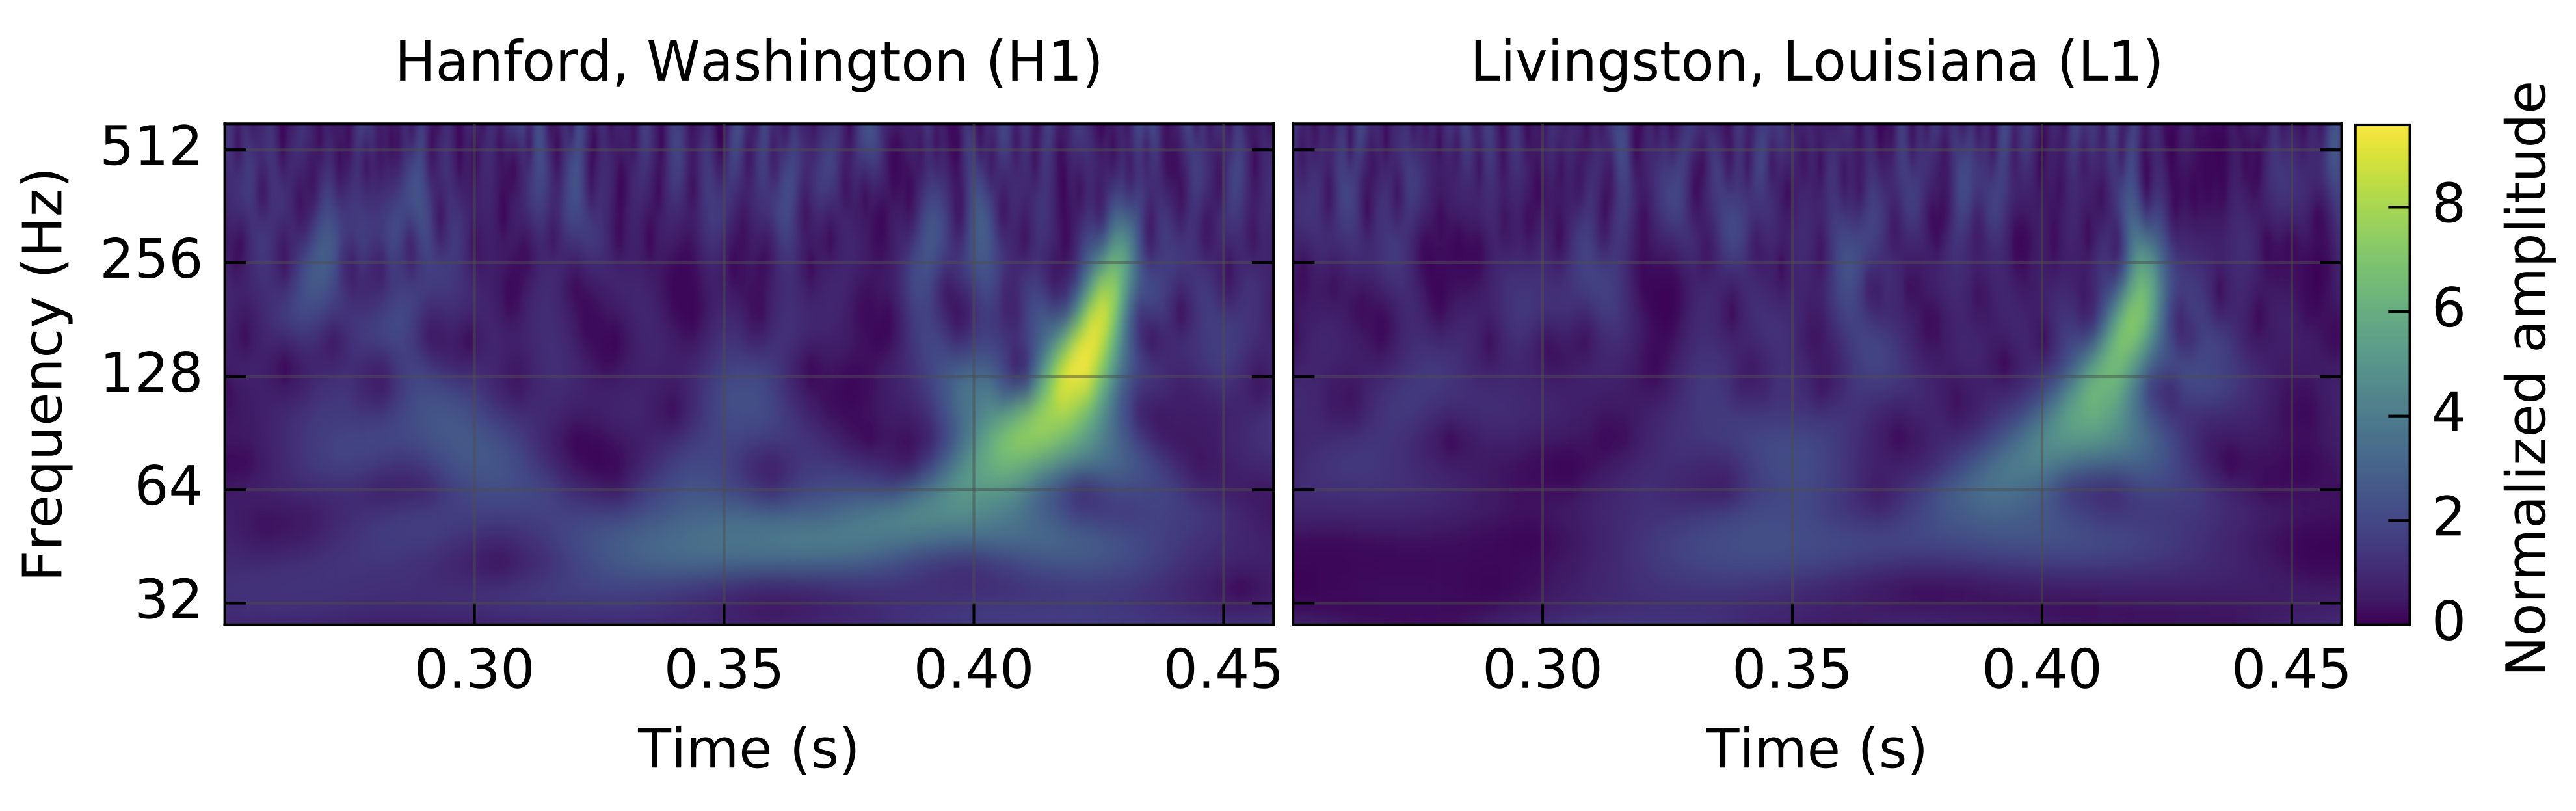
\includegraphics[width=\textwidth]{figures/GW150914.png}
    \caption{Spectrograms of GW150914, the first GW ever observed~\cite{GW150914}.}
    \label{fig:GW150914}
\end{figure*}

GW observations have already resulted in three Nobel Prizes being awarded to LIGO-affiliated physicists. So far every GW detection has originated from a compact binary system, but there are many other objects predicted to be sources of GWs. Core-collapse supernovae (CCSNe) represent one of the most promising sources of GWs yet to be observed. CCSNe can shine brightly for days, weeks, or months at a time and have been observed in the sky for thousands of years. They are also believed to be essential to our existence and way of life as they are instrumental to the spread of heavy metals throughout the universe. Despite this, the details and underlying physcis of a CCSN explosion are still somewhat mysterious. Most simulations fail to explode and there is significant uncertainty about the mechanisms and processes at work within the star in its final moments. GWs are emitted from the core of a CCSN, as opposed to electromagnetic radiation which is emitted only from the outermost layers. GWs therefore offer a unique glimpse into the heart of the star and could help physicists understand the nuclear equation of state present in a neutron star. Unfortunately, CCSNe are rare and emit weaker GWs than compact binary systems. The chances of a GW observation from a CCSN will therefore increase over the next few decades as detector sensitivities improve.

The first GW observed from a CCSN will be an important moment in astrophysics. In order to learn something from such an event, parameter estimation tools and algorithms must be developed. GWs from CCSNe are inherently random. This, in combination with the uncertainty of the underlying physics, makes parameter estimation a difficult task. This dissertation will cover my work with the LIGO collaboration with a focus on the Supernova Model Evidence Extractor (SMEE), a working parameter estimation tool for GWs from CCSNe. Chapter~\ref{GWs} will cover GWs and GW detectors. Chapter~\ref{chp:pem} will cover my work with LIGO's Physical Environment Monitoring (PEM) system. Chapter~\ref{chp:CCSNe} will cover CCSNe and their numerical relativity simulations. Chapter~\ref{chp:SMEE} will describe the SMEE algorithm in great detail, and chapter~\ref{chp:performance} will outline the performance of SMEE with an emphasis on future detectors. 
\chapter{Gravitational Waves} \label{GWs}

\section{Vectors and Tensors}

A ``four-vector", such as $V^{\nu}$, is defined as a four component vector that transforms into,
\begin{equation}
\label{equ:contra4vector}
    V'^{\mu} = V^{\nu} \frac{\partial x'^{\mu}}{\partial x^{\nu}}
\end{equation}
under a general coordinate transformation $x^{\mu} \rightarrow x'^{\mu}$. The $\alpha$ index ranges from 0\,-\,3, with 0 representing the time component and 1\,-\,3 representing the three spatial components. Throughout this thesis, Greek indices will be used to indicate four-vectors while Latin indices will represent traditional three vectors with no time component. $V^{\nu}$ in equation~\ref{equ:contra4vector} is technically a contravariant four-vector, while a covariant four-vector, such as $U_{\nu}$\,, transforms similarly,
\begin{equation}
\label{equ:cov4vector}
    U'_{\mu} = \frac{\partial x^{\nu}}{\partial x'^{\mu}} U_{\nu}
\end{equation}
A contravariant vector can be turned into a covariant vector, and vice versa, by using the metric tensor (or just metric) $g_{\mu \nu}$,
\begin{equation}
\label{equ:raise_lower}
    V_{\mu} = g_{\mu \nu}V^{\nu} \quad \text{and} \quad U^{\mu} = g^{\mu \nu}U_{\nu}
\end{equation}
The metric is extremely important in general relativity and will be elaborated on in the following section. For now, it is a matrix that can be used to raise and lower indices. The Einstein summation convention will be utilized in this dissertation, meaning that any index that simultaneously appears in the top and bottom of a formula will be summed over. As an example, $V^{\mu}U_{\mu}$ represents the dot product between a contravariant and covariant vector.

Tensors are more complicated objects that can possess multiple indices. The metric, $g_{\mu\nu}$\,, is an example of a covariant tensor since all of its indices are lowered, but tensors can also be contravariant or mixed. Identical upper and lower indices can also be summed over to produce a new tensor with fewer indices through contraction,
\begin{equation}
    T^{\alpha \gamma} = T^{\alpha\;\gamma\beta}_{\;\;\beta}
\end{equation}
The product of two tensors is a new tensor whose upper and lower indices consist of all the upper and lower indices of the original tensors,
\begin{equation}
    T^{\alpha\;\gamma}_{\;\;\beta} = A^{\alpha}_{\;\;\beta}B^{\gamma}
\end{equation}
Vectors and scalars are considered to be simple tensors with one and zero indices respectively.

\section{The Metric Tensor and Manifolds}

In the Special Theory of Relativity, the spacetime interval between two neighboring points is given by the following formula:
\begin{equation}
\label{equ:spacetime_interval}
    ds^{2} = -c^{2}dt^{2} + dx^{2} + dy^{2} + dz^{2}
\end{equation}
This can be written in a simpler form with use of the Einstein summation convention,
\begin{equation}
    ds^{2} = \eta_{\mu\nu}dx^{\mu}dx^{\nu}
\end{equation}
where $\eta_{\mu\nu}$ is the Minkowski metric representing flat spacetime. In Cartesian coordinates,
\begin{equation}
    \eta_{\mu\nu} = 
    \begin{bmatrix} 
    -1 & 0 & 0 & 0 \\
    0 & 1 & 0 & 0 \\
    0 & 0 & 1 & 0 \\
    0 & 0 & 0 & 1 \\
    \end{bmatrix}
\end{equation}
Some references flip all of the signs, but the underlying physics are unchanged. Spacetime is considered to be ``flat" if Euclid's axioms hold. This concept is typically easier to visualize in fewer dimensions. If a triangle is drawn on the surface of a sphere, as opposed to a flat piece of paper, then its angles will not sum to 180 degrees. General Relativity does not require flat spacetime and the general metric tensor, $g_{\mu\nu}$, can deviate from $\eta_{\mu\nu}$ when spacetime is curved by mass or energy.

Spacetime is said to be represented by a ``manifold". A manifold is a topological space that is locally Euclidean. The global structure of a manifold can possess curvature and be extremely complex, but at each point in spacetime a tangent vector space can be defined. Usually it is not possible to find one mapping to Euclidean space for the entire manifold and these tangent vector spaces vary for each point. This results in the concept of a straight line being poorly defined. The metric is a tensor field that defines infinitesimal distance between neighboring points of spacetime. There is a metric associated with every point in the manifold. Vectors can be measured with use of the metric in the same way that the spacetime interval was calculated in equation~\ref{equ:spacetime_interval}. More generally,
\begin{equation}
\label{equ:vector_measure}
    L = g_{\mu\nu}x^{\mu}x^{\nu} = x_{\nu}x^{\nu}
\end{equation}
In flat space, when $g_{\mu\nu} = \eta_{\mu\nu}$, equation~\ref{equ:vector_measure} reduces to the Pythagorean Theorem. A curve can be measured by integrating the infinitesimal length of tangent vectors along the curve.

The manifolds of General Relativity are smooth Riemannian manifolds, meaning that they are differentiable manifolds for which all the transition maps are smooth functions. Standard differentiation of a tensor does not always produce another tensor, but it is possible to define a covariant derivative that does. The covariant derivative will be defined in the following section.

\section{The Equivalence Principle and Equations of Motion}

The Equivalence Principle states that gravitational mass is equal to inertial mass. While considering this, Einstein realized that a static external homogeneous gravitational field could not be detected in a freely falling elevator. The statement can be expanded to include inhomogeneous fields as long as a sufficiently small region of spacetime is considered. This section will derive equations of motion in a similar fashion to Weinberg~\cite{weinberg1972gravitation}.

Consider a free particle experiencing purely gravitational forces. The Equivalence Principle tells us that there should be a freely falling coordinate system, $\xi^{\alpha}$, in which the particle's equation of motion is a straight line in spacetime. Explicitly,
\begin{equation}
\label{equ:free_fall}
    \frac{d^{2}\xi^{\alpha}}{d\tau^{2}} = 0
\end{equation}
where $d\tau$ is the proper time defined as,
\begin{equation}
    d\tau^{2} = -\eta_{\alpha\beta}d\xi^{\alpha}d\xi^{\beta}
\end{equation}
Another coordinate system, which might be at rest, accelerated, rotating, or anything else, can be defined as $x^{\mu}$. The freely falling coordinates, $\xi^{\alpha}$, are functions of $x^{\mu}$, and equation~\ref{equ:free_fall} becomes,
\begin{equation}
    \begin{split}
    0 =& \,\frac{d}{d\tau} \bigg( \frac{\partial\xi^{\alpha}}{\partial x^{\mu}} \frac{dx^{\mu}}{d\tau} \bigg) \\
    =& \,\frac{\partial\xi^{\alpha}}{\partial x^{\mu}} \frac{d^{2}x^{\mu}}{d\tau^{2}} + \frac{\partial^{2}\xi^{\alpha}}{\partial x^{\mu}\partial x^{\nu}} \frac{dx^{\mu}}{d\tau} \frac{dx^{\nu}}{d\tau}
    \end{split}
\end{equation}
Multiplying this by $\partial x^{\lambda}/\partial\xi^{\alpha}$, and using the product rule defined as,
\begin{equation}
    \frac{\partial\xi^{\alpha}}{\partial x^{\mu}} \frac{\partial x^{\lambda}}{\partial\xi^{\alpha}} = \delta^{\lambda}_{\mu}
\end{equation}
results in the following equation of motion:
\begin{equation}
    0 = \frac{d^{2}x^{\lambda}}{d\tau^{2}} + \Gamma^{\lambda}_{\mu\nu} \frac{dx^{\mu}}{d\tau} \frac{dx^{\nu}}{d\tau}
\end{equation}
where $\Gamma^{\lambda}_{\mu\nu}$ are called Christoffel symbols and are defined as,
\begin{equation}
    \Gamma^{\lambda}_{\mu\nu} = \frac{\partial x^{\lambda}}{\partial\xi^{\alpha}} \frac{\partial^{2}\xi^{\alpha}}{\partial x^{\mu}\partial x^{\nu}}
\end{equation}
The Christoffel symbols are sometimes referred to as a metric connection, and are a specialization of the affine connection. They represent a connection between surfaces or manifolds that possess a metric and allow distances to be measured on that surface. The Christoffel symbols are the field that determines the gravitational force, while the metric determines the proper time interval between two events with infinitesimal coordinate separation. The metric can also be seen as the gravitational potential, since its derivatives determine the field $\Gamma^{\lambda}_{\mu\nu}$. Writing the Christoffel symbols in terms of the metric~\cite{schutz_2009, wald},
\begin{equation}
    \Gamma^{\sigma}_{\lambda\mu} = \frac{1}{2}g^{\nu\sigma}\bigg(\frac{\partial g_{\mu\nu}}{\partial x^{\lambda}} + \frac{\partial g_{\lambda\nu}}{\partial x^{\mu}} - \frac{\partial g_{\mu\lambda}}{\partial x^{\nu}}\bigg)
\end{equation}

As stated earlier, standard differentiation of a tensor does not result in a new tensor. To define a derivative that does produce a tensor, we can start with the contravariant transformation law in equation~\ref{equ:contra4vector}. Differentiating with respect to $x'^{\lambda}$ gives,
\begin{equation}
\label{equ:vector_transform_diff}
    \frac{\partial V'^{\mu}}{\partial x'^{\lambda}} = \frac{\partial x'^{\mu}}{\partial x^{\nu}} \frac{\partial x^{\rho}}{\partial x'^{\lambda}} \frac{\partial V^{\nu}}{\partial x^{\rho}} + \frac{\partial^{2}x'^{\mu}}{\partial x^{\nu}\partial x^{\rho}} \frac{\partial x^{\rho}}{\partial x'^{\lambda}} V^{\nu}
\end{equation}
The second term on the right is what stops $\partial V^{\mu}/\partial x^{\lambda}$ from being a tensor. This derivative can, however, be used to create a tensor. To do so, we'll start with the transformation law for the Christoffel symbols. From Weinberg~\cite{weinberg1972gravitation},
\begin{equation}
    \begin{split}
    \Gamma'^{\mu}_{\lambda\kappa}V'^{\kappa} =& \,\bigg( \frac{\partial x'^{\mu}}{\partial x^{\nu}} \frac{\partial x^{\rho}}{\partial x'^{\lambda}} \frac{\partial x^{\sigma}}{\partial x'^{\kappa}} \Gamma^{\nu}_{\rho\sigma} - \frac{\partial^{2}x'^{\mu}}{\partial x^{\rho}x^{\sigma}} \frac{\partial x^{\rho}}{\partial x'^{\lambda}} \frac{\partial x^{\sigma}}{\partial x'^{\kappa}} \bigg) \frac{\partial x'^{\kappa}}{\partial x^{\eta}}V^{\eta} \\
    =& \,\frac{\partial x'^{\mu}}{\partial x^{\nu}} \frac{\partial x^{\rho}}{\partial x'^{\lambda}} \Gamma^{\nu}_{\rho\sigma}V^{\sigma} - \frac{\partial^{2}x'^{\mu}}{\partial x^{\rho}\partial x^{\sigma}} \frac{\partial x^{\rho}}{\partial x'^{\lambda}}V^{\sigma}
    \end{split}
\end{equation}
When adding this to equation~\ref{equ:vector_transform_diff} the inhomogeneous terms (rightmost terms in both equations) cancel, resulting in:
\begin{equation}
    \frac{\partial V'^{\mu}}{\partial x'^{\lambda}} + \Gamma'^{\mu}_{\lambda\kappa}V'^{\kappa} = \frac{\partial x'^{\mu}}{\partial x^{\nu}} \frac{\partial x^{\rho}}{\partial x'^{\lambda}} \bigg(\frac{\partial V^{\nu}}{\partial x^{\rho}} + \Gamma^{\nu}_{\rho\sigma}V^{\sigma} \bigg)
\end{equation}
This can be rewritten as,
\begin{equation}
\label{equ:cov_transform}
    V'^{\mu}_{\;\;\;\;;\lambda} = \frac{\partial x'^{\mu}}{\partial x^{\nu}} \frac{\partial x^{\rho}}{\partial x'^{\lambda}}V^{\nu}_{\;\;\;;\rho}
\end{equation}
where 
\begin{equation}
\label{equ:cov_deriv}
    V^{\mu}_{\;\;\;;\lambda} = \frac{\partial V^{\mu}}{\partial x^{\lambda}} + \Gamma^{\mu}_{\lambda\kappa}V^{\kappa}
\end{equation}
Equation~\ref{equ:cov_deriv} defines the covariant derivative. This derivative is represented with a semicolon and produces a tensor, as can be seen from the transformation in equation~\ref{equ:cov_transform}. A similar formula defines the covariant derivative for covariant vectors,
\begin{equation}
    V_{\mu;\nu} = \frac{\partial V_{\mu}}{\partial x^{\nu}} - \Gamma^{\lambda}_{\mu\nu}V_{\lambda}
\end{equation}

\section{The Einstein Field Equations}

Mass, or energy, can be seen as the ``charge" for gravitational forces. This differentiates gravity from electromagnetism because gravitational fields carry energy and momentum, whereas electromagnetic fields do not carry a charge. This means that gravitational fields contribute to their own sources, and that the field equations of General Relativity will be nonlinear partial differential equations, as opposed to the linear formulas found in Maxwell's equations. Einstein's field equations take the form:
\begin{equation}
\label{equ:field}
    R_{\mu\nu} - \frac{1}{2}g_{\mu\nu}R + \Lambda g_{\mu\nu} = \frac{8\pi G}{c^{4}} T_{\mu\nu}
\end{equation}
$R_{\mu\nu}$ is the Ricci curvature tensor, $R$ is the scalar curvature, $g_{\mu\nu}$ is the metric tensor, $\Lambda$ is the cosmological constant, $G$ is Newton's gravitational constant, and $T_{\mu\nu}$ is the stress-energy tensor. Equation~\ref{equ:field} has been written in SI units, but it is also commonly written in natural (or geometrized) units with $c = G = 1$. Each term will be defined below.

The Ricci curvature tensor is one way of representing how the geometry of a metric differs from Euclidean space. It can be described as the part of spacetime curvature that determines the degree to which matter will tend to converge or diverge in time. It is also a trace of the Riemann curvature tensor, which is defined as:
\begin{equation}
\label{equ:riemann_curv_tensor}
    R^{\lambda}_{\;\;\mu\nu\kappa} = \frac{\partial \Gamma^{\lambda}_{\mu\nu}}{\partial x^{\kappa}} - \frac{\partial \Gamma^{\lambda}_{\mu\kappa}}{\partial x^{\nu}} + \Gamma^{\eta}_{\mu\nu}\Gamma^{\lambda}_{\kappa\eta} - \Gamma^{\eta}_{\mu\kappa}\Gamma^{\lambda}_{\nu\eta}
\end{equation}
The Riemann curvature tensor is the only tensor that can be constructed from the metric tensor and its first two derivatives. It is the most commonly used tensor to represent spacetime curvature and it measures the extent to which the metric tensor is not locally isometric to that of Euclidean space. Taking the trace results in the Ricci tensor,
\begin{equation}
    R_{\mu\nu} = R^{\lambda}_{\;\;\mu\lambda\nu}
\end{equation}
Just as the Ricci curvature tensor is the trace of the Riemann curvature tensor, the trace of the Ricci tensor produces $R$, the scalar curvature. 
\begin{equation}
    R = g^{\mu\nu}R_{\mu\nu}
\end{equation}
The scalar curvature is the simplest curvature invariant of a Riemannian manifold. In a geometric sense, it represents the amount by which the volume of a small geodesic ball in a Riemannian manifold differs from that of the standard ball in Euclidean space. The left side of equation~\ref{equ:field} is sometimes simplified by defining the Einstein tensor, $G_{\mu\nu}$, which includes both curvature terms,
\begin{equation}
    G_{\mu\nu} = R_{\mu\nu} - \frac{1}{2}g_{\mu\nu}R
\end{equation}

The cosmological constant term was originally added by Einstein to produce a static universe. It was eventually removed from his field equations after Hubble discovered that the universe was expanding in 1931. Modern research has shown that the expansion of the universe appears to be accelerating, causing the cosmological constant to be once again added to Einstein's field equations. It is now interpreted as the energy density of space (also vacuum energy) and is closely related to the somewhat mysterious concept of dark energy. The last significant term in equation~\ref{equ:field} is $T_{\mu\nu}$, the stress-energy tensor. The stress-energy tensor is the source of gravitational fields in General Relativity, in the same way that the mass density is the source of Newtonian gravity. It describes the density and flux of energy and momentum in spacetime, and is therefore affected by matter, radiation, and the fields of non-gravitational forces. The stress-energy tensor can take various forms, but one of the most common represents a perfect fluid in thermodynamic equilibrium,
\begin{equation}
\label{equ:stress_energy_tensor}
    T^{\mu\nu} = \Big(\rho + \frac{p}{c^{2}}\Big)u^{\mu}u^{\nu} + pg^{\mu\nu}
\end{equation}
where $\rho$ is the mass-energy density, $p$ is the hydrostatic pressure, $u^{\mu}$ is the fluid's four-velocity, and $g^{\mu\nu}$ is the inverse of the standard metric.

\subsection{Weak Field Approximation}

Many calculations related to GWs are performed in the weak field limit where spacetime is approximately flat~\cite{flanagan2005basics}. This is also called ``linearized gravity" because Einstein's field equations become linear differential equations. The metric takes the form of the Minkowski metric with a small perturbation $h_{\mu\nu}$,
\begin{equation}
    g_{\mu\nu} = \eta_{\mu\nu} + h_{\mu\nu} \quad\quad \text{with} \quad\quad |h_{\mu\nu}| \ll 1
\end{equation}
Because the perturbations are small, only terms linear in $h_{\mu\nu}$ must be considered and higher order terms can be dropped as they are negligible. When working in this domain, indices are raised and lowered with the Minkowski metric. For simplicity, partial derivatives will be written as: $\partial_{\alpha} = \partial / \partial x^{\alpha}$. The Christoffel symbols then take the form,
\begin{equation}
    \begin{split}
    \Gamma^{\alpha}_{\beta\gamma} =& \,\frac{1}{2}\eta^{\alpha\lambda}\big(\partial_{\gamma}h_{\lambda\beta} + \partial_{\beta}h_{\lambda\gamma} - \partial_{\lambda}h_{\beta\gamma}\big) \\
    =& \,\frac{1}{2}\big(\partial_{\gamma}h^{\alpha}_{\;\;\beta} + \partial_{\beta}h^{\alpha}_{\;\;\gamma} - \partial^{\alpha}h_{\beta\gamma}\big)
    \end{split}
\end{equation}
The Riemann tensor can then be written as,
\begin{equation}
    \begin{split}
    R^{\alpha}_{\;\;\beta\gamma\lambda} =& \,\partial_{\gamma}\Gamma^{\alpha}_{\beta\lambda} - \partial_{\lambda}\Gamma^{\alpha}_{\beta\gamma} \\
    =& \,\frac{1}{2}\big(\partial_{\gamma}\partial_{\beta}h^{\alpha}_{\;\;\lambda} + \partial_{\lambda}\partial^{\alpha}h_{\beta\gamma} - \partial_{\gamma}\partial^{\alpha}h_{\beta\lambda} - \partial_{\lambda}\partial_{\beta}h^{\alpha}_{\;\;\gamma}\big)
    \end{split}
\end{equation}
From this, the Ricci tensor can be constructed,
\begin{equation}
    R_{\alpha\beta} = R^{\gamma}_{\;\;\alpha\gamma\beta} = \frac{1}{2}\big(\partial_{\gamma}\partial_{\beta}h^{\gamma}_{\;\;\alpha} + \partial^{\gamma}\partial_{\alpha}h_{\beta\gamma} - \square h_{\alpha\beta} - \partial_{\alpha}\partial_{\beta}h\big)
\end{equation}
where $h = h^{\alpha}_{\;\;\alpha}$ is the trace of the metric perturbation and $\square = \partial_{\alpha}\partial^{\alpha} = \nabla^{2} - \partial^{2}_{t}$ is the wave operator, also known as the d'Alembertian. The scalar curvature can be found by contracting once more,
\begin{equation}
    R = R^{\alpha}_{\;\;\alpha} = \big(\partial_{\gamma}\partial^{\alpha}h^{\gamma}_{\;\;\alpha} - \square h\big)
\end{equation}
Finally, these results can be combined to produce the Einstein tensor,
\begin{equation}
\label{equ:ein_tensor_lin}
    \begin{split}
    G_{\alpha\beta} =& \,R_{\alpha\beta} - \frac{1}{2}\eta_{\alpha\beta}R \\
    =& \,\frac{1}{2}\big(\partial_{\gamma}\partial_{\beta}h^{\gamma}_{\;\;\alpha} + \partial^{\gamma}\partial_{\alpha}h_{\beta\gamma} - \square h_{\alpha\beta} - \partial_{\alpha}\partial_{\beta}h - \eta_{\alpha\beta}\partial_{\gamma}\partial^{\lambda}h^{\gamma}_{\;\;\lambda} + \eta_{\alpha\beta}\square h\big)
    \end{split}
\end{equation}
This expression can be simplified by introducing the trace-reversed perturbation $\overline{h}_{\alpha\beta} = h_{\alpha\beta} - \frac{1}{2}\eta_{\alpha\beta}h$. This notation obtains its name from the fact that $\overline{h}^{\alpha}_{\;\;\alpha} = -h$. All terms with the trace $h$ cancel when replacing $h_{\alpha\beta}$ with $\overline{h}_{\alpha\beta} + \frac{1}{2}\eta_{\alpha\beta}h$ in equation~\ref{equ:ein_tensor_lin},
\begin{equation}
\label{equ:einstein_tensor_linearized}
    G_{\alpha\beta} = \frac{1}{2}\big(\partial_{\gamma}\partial_{\beta}\overline{h}^{\gamma}_{\;\;\alpha} + \partial^{\gamma}\partial_{\alpha}\overline{h}_{\beta\gamma} - \square \overline{h}_{\alpha\beta} - \eta_{\alpha\beta}\partial_{\gamma}\partial^{\lambda}\overline{h}^{\gamma}_{\;\;\lambda}\big)
\end{equation}
This result can be further simplified by choosing the correct coordinates, or gauge. It is always possible to transform into the Lorentz gauge, defined as,
\begin{equation}
\label{equ:lorentz_gauge}
    \partial^{\alpha}\overline{h}_{\alpha\beta} = 0
\end{equation}
When applying the Lorentz gauge to equation~\ref{equ:einstein_tensor_linearized}, all terms but one vanish, giving the result,
\begin{equation}
    G_{\alpha\beta} = -\frac{1}{2}\square \overline{h}_{\alpha\beta}
\end{equation}
Therefore, in the weak field approximation, Einstein's field equations reduce to,
\begin{equation}
\label{equ:weak_field_einstein}
    \square \overline{h}_{\alpha\beta} = -16\pi T_{\alpha\beta}
\end{equation}
Equation~\ref{equ:weak_field_einstein} has been written in natural units with $c = G = 1$. In a vacuum, $T_{\alpha\beta} = 0$, and the field equations reduce even further to a standard wave equation,
\begin{equation}
    \square \overline{h}_{\alpha\beta} = 0
\end{equation}
Far from an energetic source, the metric perturbation propagates as a plane wave and has solutions of the form,
\begin{equation}
    h = Ae^{i(2\pi ft-\mathbf{k}\cdot\mathbf{r})}
\end{equation}
where $A$ is the wave amplitude, $f$ is the wave frequency, $k$ is the wave number ($2\pi f/c$), and the wave propagates in the direction $\hat{k}$.

\section{Gravitational Radiation}

A full derivation of GW emission can be found in many relativity texts~\cite{gravitation, schutz_2009, wald, weinberg1972gravitation}, but this process is quite rigorous and in most situations (when the size of the source is much smaller than the wavelength, $r_{\text{source}}/\lambda \ll 1$) a multipole expansion approximation is sufficient. It is helpful to compare the emission of GW radiation to the emission of electromagnetic radiation in a similar fashion to Saulson~\cite{bible}. The dominant contribution comes from time derivatives of the dipole moment and takes the form,
\begin{equation}
\label{equ:em_radiation}
    \mathbf{E} = \frac{1}{Rc^{2}}\big(\ddot{\mathbf{d}} \times \mathbf{n}\big) \times \mathbf{n}
\end{equation}
where $R$ is the distance from the source to the observation point, $\mathbf{n}$ is the unit vector pointing from the source to the observer, and $\mathbf{d}$ is the electric dipole moment defined as,
\begin{equation}
    \mathbf{d} = \int dV\rho_{q}(\mathbf{r})\mathbf{r}
\end{equation}
There is no electromagnetic monopole radiation because that would require a time derivative of the monopole moment, also known as the total electric charge of the source. Isolated systems cannot change their total charge, and so monopole radiation is prohibited. The movement of charges within the source is expressed in the dipole and higher moments of the expansion.

There are important similarities and differences between gravity and electromagnetism that must be considered when trying to produce analogous radiation formulas. The most obvious difference being that electromagnetism possesses two charges while gravity possesses only one. Monopole radiation can be immediately eliminated as a source of GWs due to the conservation of energy, which is analogous to the conservation of charge in electromagnetism. It is easy enough to define a gravitational dipole moment, $\mathbf{d}_{g}$, but this radiation can also be eliminated as the conservation of momentum requires that $\dot{\mathbf{d}}_{g}$ remain constant. It is also possible to define a gravitational analog of the magnetic dipole moment, but this also must remain constant due to the conservation of angular momentum. Gravitational radiation must therefore depend on the quadrupole and higher moments. It is common to define the reduced quadrupole moment as,
\begin{equation}
    I_{\mu\nu} = \int dV\big(x_{\mu}x_{\nu} - \frac{1}{3}\delta_{\mu\nu}r^{2}\big)\rho\big(\mathbf{r}\big)
\end{equation}
The gravitational analog of equation~\ref{equ:em_radiation} can now be written for quadrupole radiation,
\begin{equation}
\label{equ:amp_radiation}
    h_{\mu\nu} = \frac{2G}{Rc^{4}} \ddot{I}_{\mu\nu}
\end{equation}
Equation~\ref{equ:amp_radiation} has been written in SI units and represents the strongest contribution to GW emission. One of the simplest and most important cases is GW emission from an orbiting binary system, for which the amplitude of emission takes the form,
\begin{equation}
    |h| = \frac{r_{S1}r_{S2}}{r_{0}R}
\end{equation}
where $r_{S1}$ and $r_{S2}$ are the radii of the two objects, and $2r_{0}$ is the distance between them.

Most calculations related to GWs are performed in the transverse traceless (TT) gauge, which is a further specialization of the Lorentz gauge requiring that the metric perturbation be purely spatial,
\begin{equation}
    h_{tt} = h_{ti} = 0
\end{equation}
and traceless,
\begin{equation}
    h = h_{i}^{\;\;i} = 0
\end{equation}
In combination with the Lorentz gauge (equation~\ref{equ:lorentz_gauge}), this requires the spatial metric perturbation to be transverse,
\begin{equation}
    \partial_{i}h_{ij} = 0
\end{equation}
For a wave travelling in the $\hat{z}$ direction, the TT gauge requires that the metric perturbation take the form,
\begin{equation}
    h_{\mu\nu} = 
    \begin{bmatrix} 
    0 & 0 & 0 & 0 \\
    0 & a & b & 0 \\
    0 & b & -a & 0 \\
    0 & 0 & 0 & 0 \\
    \end{bmatrix}
\end{equation}
This can then be written as the sum of two components, $h = a\hat{h}_{+} + b\hat{h}_{\times}$, where
\begin{equation}
    h_{+} = 
    \begin{bmatrix} 
    0 & 0 & 0 & 0 \\
    0 & 1 & 0 & 0 \\
    0 & 0 & -1 & 0 \\
    0 & 0 & 0 & 0 \\
    \end{bmatrix} \quad\quad \text{and} \quad\quad
    h_{\times} = 
    \begin{bmatrix} 
    0 & 0 & 0 & 0 \\
    0 & 0 & 1 & 0 \\
    0 & 1 & 0 & 0 \\
    0 & 0 & 0 & 0 \\
    \end{bmatrix}
\end{equation}
The plus and cross polarizations represent two orthogonal polarizations for waves propagating in the $\hat{z}$ direction. Gravitation in General Relativity isn't really a traditional force, instead it should be viewed as a manifestation of geodesic motion in curved spacetime. The $h_{+}$ polarization of a passing wave shrinks and elongates the $\hat{x}$ and $\hat{y}$ dimensions, while the $h_{\times}$ polarization does the same with its axis rotated 45 degrees. The effect of a passing GW on a circular ring of test masses can be seen in Figure~\ref{fig:passing_GW}. This changing of distance between freely falling test masses is essential to the function of GW detectors.

\begin{figure*}[b!]
    \centering
    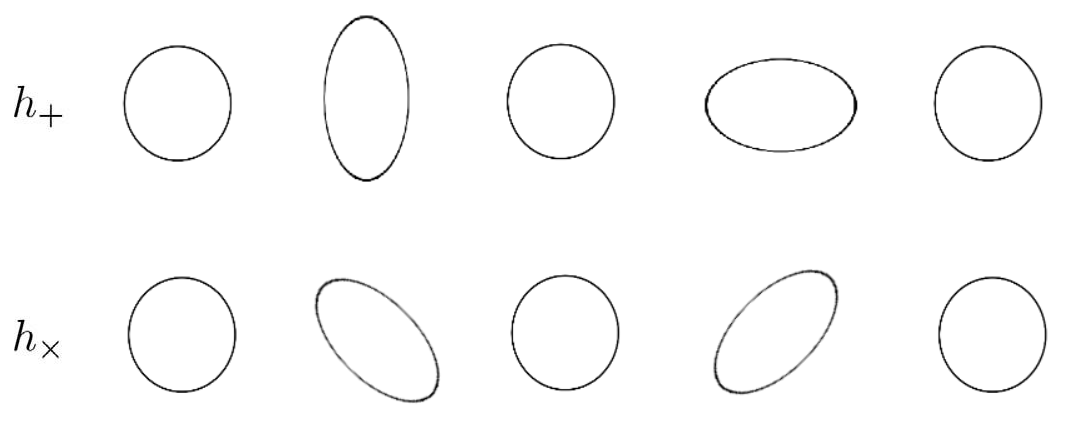
\includegraphics[width=\textwidth]{figures/passing_GW.png}
    \caption{The effect of a passing GW on a circular ring of test masses. The $h_{+}$ and $h_{\times}$ polarizations differ in their action by a rotation of 45 degrees.}
    \label{fig:passing_GW}
\end{figure*}

\subsection{Sources of Gravitational Waves}

Because quadrupole emission is the dominant source of GWs, any highly energetic astronomical events with asymmetric motion are expected to produce significant radiation. This section will briefly describe the main sources of GWs that LIGO and future detectors hope to study.

\subsection{Compact Binary Coalescences}

CBC signals are currently the most important source of GWs as they are the only ones that have been observed through LIGO's first two observing runs~\cite{GW150914, abbott2016binary, abbott2017gw170817}. Two compact objects, such as black holes or neutron stars, produce strong emission as they orbit each other in a configuration that is inherently quadrupolar. The frequency of GW emission increases over time as the two masses get closer, culminating in a ``chirp" right before coalescence. Current GW detectors have been constructed to be most sensitive to these final few seconds of orbit as the amplitude of emission is strongest. All but one of LIGO's GW observations have been from binary black hole (BBH) mergers. GW170817 is the lone exception and contained the signal from a binary neutron star (BNS) merger~\cite{abbott2017gw170817}. GW170817 was also accompanied by an electromagnetic counterpart known as a gamma-ray burst (GRB), initiating the era of multi-messenger astronomy.

CBC signals can be modeled very accurately in numerical relativity simulations, which allows CBC searches to utilize a technique known as matched filtering. Matched filtering is an effective technique for finding quiet signals but can only be employed when the waveform is well known. Template waveforms, representing different source parameters, are moved across detector data while calculating the cross-correlation. At each point in time an SNR, $\rho$, is calculated as,
\begin{equation}
    \rho^{2} = 4\int_{0}^{\infty} \frac{\Tilde{d}(f)\Tilde{h}^{\ast}(f)}{S(f)}df
\end{equation}
where $S(f)$ is the one-sided noise power spectral density, $\Tilde{d}$ represents detector data, and $\Tilde{h}$ is the template waveform. This SNR will spike if the template waveform appears in the detector data. For the rest of this thesis, any references to SNR will be referring to this matched filter SNR.

\subsection{Bursts}

Bursts are transient GW signals with imprecise or unknown waveforms. Because the waveforms are not precisely known, matched filter searches cannot be implemented. Examples of burst sources include CBC mergers with unusually high mass ratios or eccentricity, cosmic strings, gamma-ray bursts, and CCSNe. Supernovae will covered in great detail in chapter~\ref{chp:CCSNe}.

Burst searches typically look for excess power events that are coherent between multiple detectors. These can be generic searches through all detector data, or targeted searches based off of astronomical observations. For example, electromagnetic and neutrino observations are both used for targeted CCSN searches. There are two independent burst search algorithms, Coherent Wave-burst~\cite{klimenko2008coherent}, and Omicron-LALInference-Burst~\cite{lynch2017information}. Algorithms such as BayesWave~\cite{cornish2015bayeswave} and SMEE~\cite{roma2019astrophysics} (the subject of this thesis) are then used to reconstruct and study the GW signals. It is usually difficult to extract useful source parameters from a burst signal, but the GW amplitude, duration, and frequency content can typically be estimated.

\subsection{Continuous Waves}

Continuous GWs can be emmitted from rapidly rotating dense objects called neutron stars (also called pulsars). Neutron starts are the densest objects in the universe other than black holes. If a mountain or deformation exists on the surface of a rapidly roating neutron star then GWs can be continuously emitted due to the changing quadrupole moment. Neutron stars generally emit electromagnetic signals as well as GWs, allowing for targeted searches based off of X-ray, radio, and gamma-ray observations. Upper limits have been put on these sources with past searches~\cite{abbott2017first}. A detection of continuous GWs from a pulsar could be important as it could help determine the neutron star equation of state. GWs of this type would show up as narrow ``lines" in detector data. These searches are therefore detrimentally affected by continuous environmental noise sources.  This will be discussed further in chapter~\ref{chp:pem}.

\subsection{Stochastic Background}

In the same way that the Cosmic Microwave Background (CMB) allows scientists to look back at early moments of the universe through electromagnetic radiation, it is expected that GWs will have their own observable background. These waves began travelling when the universe became optically thin to GWs after the big bang. Observations of this stochastic background would be a watershed moment for physics/cosmology and would allow early universe theories to be tested~\cite{regimbau2011astrophysical}. Cosmic strings and binary systems (with black holes, neutron stars, and white dwarfs) are also expected to contribute to a GW background. Background signals are expected to be below LIGO's sensitive frequency band but are a promising source for future space-based detectors~\cite{ungarelli2001studying}.

\section{The Advanced LIGO Detectors}

\begin{figure*}[b!]
    \centering
    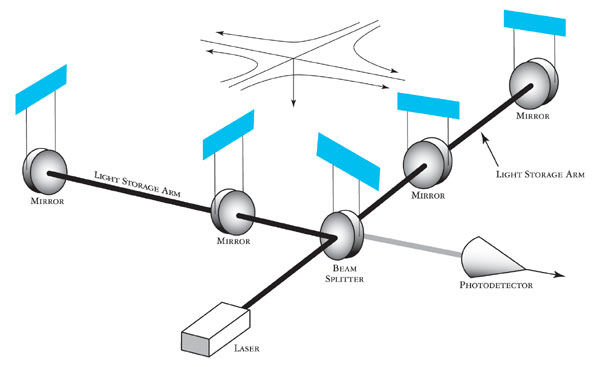
\includegraphics[width=4.5in]{figures/interferometer_diagram.jpg}
    \caption{A diagram of the Advanced LIGO detectors. Each detector is a Michelson interferometer with two Fabry-Perot cavities. Figure reproduced from~\cite{int_diagram_source}.}
    \label{fig:interferometer_diagram}
\end{figure*}

The Advanced LIGO detectors are Michelson interferometers designed to measure minute changes of length in perpendicular directions. Each L-shaped detector has two 4\,km arms referred to as x and y. Figure~\ref{fig:interferometer_diagram} shows a diagram of this arrangement. A beam of laser light ($\lambda = 1064$\,nm) passes through a central beam splitter so that half of the power enters each arm. Each arm is a resonant Fabry-Perot cavity that increases the laser power and effective detector response. Suspended mirrors (also called test masses) reflect light back and forth an average of 280 times, increasing the travel distance from 4\,km to 1120\,km. The light is then recombined at the output port to produce an interference pattern. Any change in respective length between the two arms will result in a phase change between light from the x-arm and light from the y-arm. This phase difference changes the brightness of fringes in the interference pattern and allows gravitational strain to be measured. Strain is a unitless quantity defined as the change in length over original length,
\begin{equation}
    h = \frac{\Delta L}{L}
\end{equation}
The Advanced LIGO detectors are the most sensitive rulers ever built and can detect changes of length on the order of $1\times10^{-19}$\,m, a distance 10,000 times smaller than the diameter of a proton. The sensitive frequency band of the LIGO detectors is approximately 30\,-\,3000\,Hz. The maximum sensitivity occurs at a frequency with wavelength roughly equal to the distance probed by the time of flight of the lasers, $f = c/(2\pi L)$. For the Advanced LIGO detectors this is approximately 120\,Hz.

\begin{figure*}[b!]
    \centering
    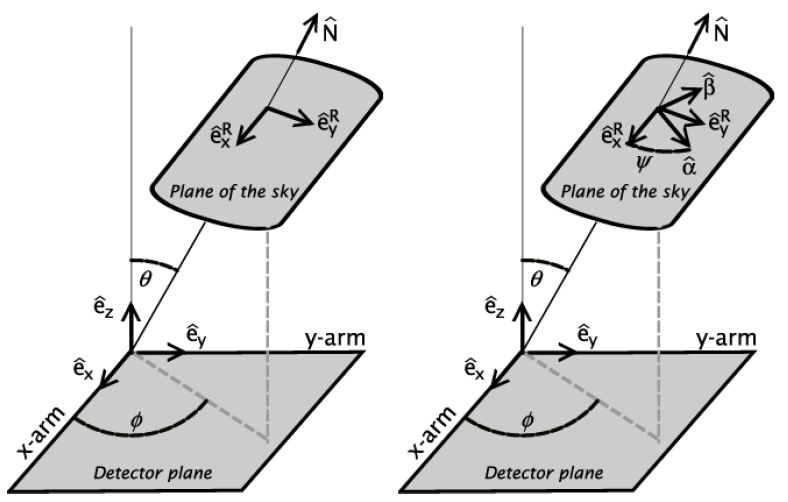
\includegraphics[width=5in]{figures/source_orientation.png}
    \caption{Left: Orientation of source and detector frames. Right: The effect of a
rotation by the angle $\psi$ in the sky frame. Image reproduced from~\cite{sathyaprakash2009physics}.}
    \label{fig:source_orientation}
\end{figure*}

The sensitivity of an interferometer depends on the orientation and sky location of the source. Figure~\ref{fig:source_orientation} shows the standard definitions for detector and source coordinates. The gravitational wave strain can be written as a sum of the two GW polarizations,
\begin{equation}
    h = F_{+}(\theta, \phi, \psi)h_{+} + F_{\times}(\theta, \phi, \psi)h_{\times}
\end{equation}
where $F_{+}$ and $F_{\times}$ are the antenna response functions. With the definitions in Figure~\ref{fig:source_orientation}, the antenna response functions can be written as,
\begin{equation}
    F_{+} = \frac{1}{2}(1+\cos^{2}\theta)\cos2\phi\cos2\psi - \cos\theta\sin2\phi\sin2\psi
\end{equation}
\begin{equation}
    F_{\times} = \frac{1}{2}(1+\cos^{2}\theta)\cos2\phi\cos2\psi + \cos\theta\sin2\phi\sin2\psi
\end{equation}
Figure~\ref{fig:antenna_pattern} contains a plot of the antenna patterns. The LIGO interferometers are most sensitive to sources above and below the detector arms.

\begin{figure*}[b!]
    \centering
    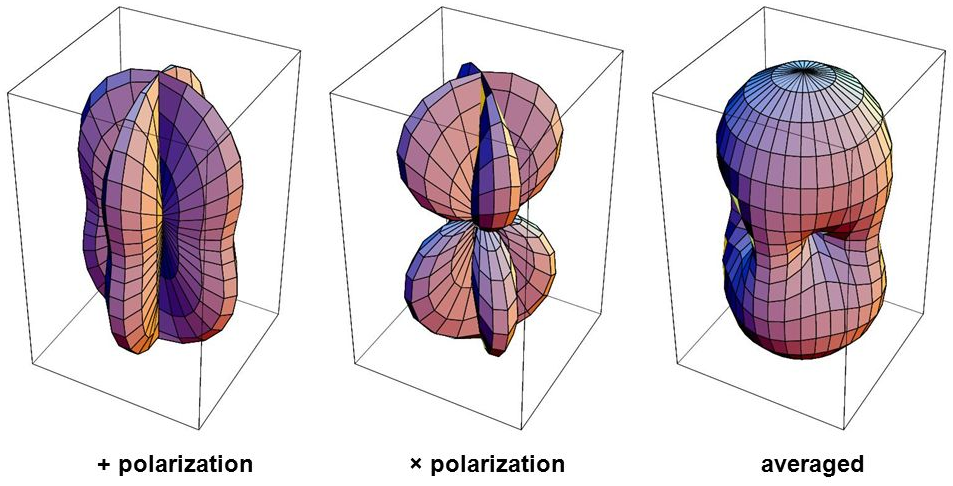
\includegraphics[width=4in]{figures/antenna_pattern.png}
    \caption{Antenna response patterns for the $h_{+}$ and $h_{\times}$ polarizations. Image reproduced from~\cite{antenna_pattern}.}
    \label{fig:antenna_pattern}
\end{figure*}

While the LIGO interferometers are relatively easy to understand in principle, there are many details and difficulties that arise in practice. Each 4\,km arm must be entirely contained in a vacuum, making the LIGO detectors the largest surface area vacuums on earth. The test masses, along with various other optics and electronics, are also contained within large vacuum chambers. Figure~\ref{fig:pem_website}, later in this dissertation, shows the locations of these chambers. Within these chambers, the test masses hang from multiple attached pendulums, which serve as passive isolation against seismic or other motion. Active isolation systems, referred to as HEPI systems~\cite{matichard2015seismic}, further reduce seismic noise and ground motion. Before the laser light enters the Fabry-Perot cavities it passes through a bow-tie shaped mirror configuration known as the Input Mode Cleaner. This serves to remove any frequencies of light differing from 1064\,Hz. A similar mirror configuration, called the Output Mode Cleaner, is located right before the final readout.

\subsection{Noise Sources}

Many different noise sources can limit the performance of GW detectors. Figure~\ref{fig:noise_budget} summarizes the main contributors to Advanced LIGO's noise budget. At low frequencies ($\lesssim 10$\,Hz) seismic ground motion is the largest noise source. Ground motion can propagate through the stages supporting the suspensions and the suspensions themselves. Active noise isolation plays a big part in reducing the seismic contribution, differentiating the Advanced LIGO detectors from earlier LIGO detectors. Shot noise is a quantum noise effect caused by a limited number of photons in a beam~\cite{buonanno2001quantum}. This is the dominant noise source at high frequencies above LIGO's most sensitive band. Shot noise can be reduced with higher laser power (more photons), but that in turn increases radiation pressure on the test masses as well as thermal noise within the test masses. Radiation pressure is the pressure imparted on a mass due to its interaction with photons~\cite{dooley2013angular}. Thermal noise due to Brownian motion in the optical coatings is a significant noise source in the most sensitive frequency range of the instruments~\cite{evans2008thermo}. Thermal energy can also be dissipated through the fibers that connect the suspension stages~\cite{saulson1990thermal}. Optical coating Brownian noise and suspension thermal noise both depend on the properties of the materials used. Gravity gradient noise is caused by fluctuations in the local gravitational field due to variations in the distribution of matter near the interferometer. This noise is potentially dominant below about 1\,Hz, well below the sensitive band of Advanced LIGO~\cite{driggers2012subtraction}.

\begin{figure*}[t]
    \centering
    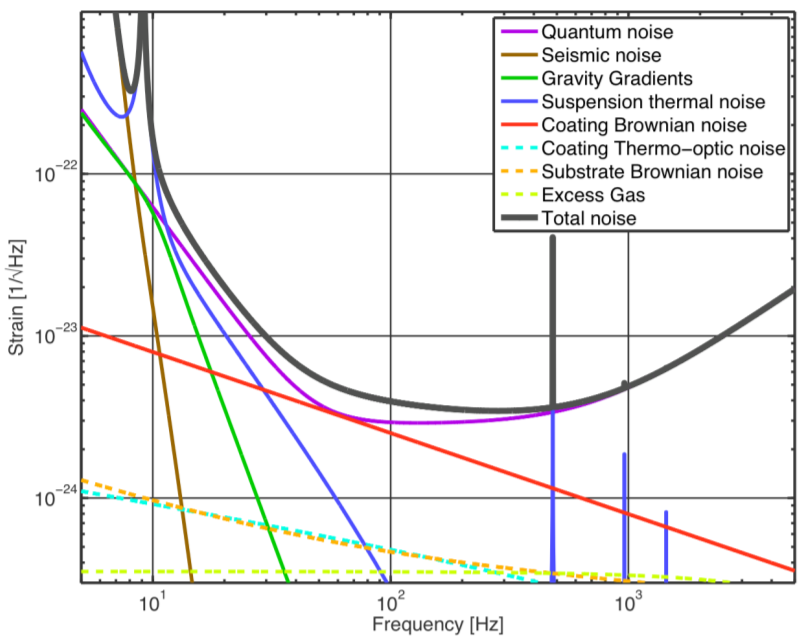
\includegraphics[width=4in]{figures/noise_budget.png}
    \caption{Advanced LIGO noise budget. Image reproduced from~\cite{whitepaper2018}.}
    \label{fig:noise_budget}
\end{figure*}

During O1 and O2 there was some mystery noise in the LIGO detectors at low frequencies. This may have been related to the sensing and control systems, the environment, or some source not previously conceived. Small amounts of uncertain noise are an unfortunate reality due to the complexity of interferometers, where each part of the detector is intricately coupled to very other part. Fluctuations in laser power (or frequency) and angular drift of the optics can also potentially contribute to detector noise. Glitches are transient noise artifacts that temporarily disrupt LIGO's data. They can be instigated by electronics or by the environment. Whenever possible, the sources of these glitches are removed. When it's not possible to do so, the glitches must be characterized and understood in order to differentiate them from possible GW signals. Glitches, and environmental noise in general, will be expanded upon in chapter~\ref{chp:pem}.

\section{Future Gravitational Wave Detectors}

This section will describe future GW detectors planned to be built over the next few decades.

\subsection{A+}

LIGO A+ is a relatively modest set of planned upgrades to the Advanced LIGO detectors in Livingston, LA and Hanford, WA~\cite{miller2015prospects}. The improvements of A+ are focused on Advanced LIGO's dominant noise sources, quantum noise and coating thermal noise. This potentially includes the installation of a squeezed light source with a filter cavity, and new end-test-masses (and possibly input-test-masses) with improved coatings. Low-risk upgrades to the suspensions may also be made, such as modifications to reduce gas damping, improve bounce and roll mode damping, mitigate parametric instabilities, etc~\cite{whitepaper2018}.

\subsection{Advanced Virgo}

Virgo is a 3\,km interferometer operating out of Italy~\cite{AdVirgo}. It was initially constructed in 2003 and has recently undergone various upgrades to become Advanced Virgo. Advanced Virgo began commissioning in 2016 and participated in the second observing run (O2) with the Advanced LIGO detectors. Three major upgrades were been performed in preparation for O3. It is had upgraded its input laser to higher power, replaced its steel test mass suspension wires with ones made of fused silica, and added a squeezed vacuum source at the output of the interferometer. These upgrades have resulted in Advanced Virgo approaching design sensitivity~\cite{AdVirgo, whitepaper2018}.

\subsection{Kagra}

Kagra is a 3\,km long underground interferometer built in the Kamioka mine in Japan~\cite{2013PhRvD..88d3007A, aso2013interferometer}. It is similar in design to other existing detectors but is built underground to minimize seismic noise, gravity gradient noise, and other environmental fluctuations such as temperature and humidity~\cite{Somiya2012detector}. Advanced LIGO and Advanced Virgo both use fused silica test masses at room temperature, while Kagra uses sapphire test masses at 20\,K to reduce thermal noise. Kagra will serve as a test case and pioneer for future detectors that also incorporate underground construction and cryogenic cooling. Kagra is expected to begin observing runs as early as 2020~\cite{2013PhRvD..88d3007A, Somiya2012detector, aso2013interferometer}.

\subsection{Voyager}

LIGO Voyager is a proposed upgrade to the Advanced LIGO detectors based on LIGO's `Blue' design concept~\cite{voyagerupgrade}. The detectors are expected to be operational by 2030~\cite{whitepaper2018}. LIGO Voyager's main modifications may include 120 - 200 kg Silicon test masses, amorphous-silicon multi-layer coatings for reduced thermal noise, low temperature ($\sim123$ K) cryogenic operation of the test masses, silicon ribbons for the final stage of test mass suspension, 200\,W pre-stabilized laser with a $\sim2000$ nm wavelength, squeezed light injection in combination with a squeezed light filter cavity, and Newtonian Gravity noise subtraction by seismometer arrays and adaptive filtering~\cite{2015PhRvD..91h2001D, whitepaper2018}.

\subsection{Einstein Telescope}

The Einstein Telescope (ET) is a proposed underground detector expected to be built in Europe~\cite{0264-9381-27-19-194002}. The current design is an equilateral triangle with 10\,km long arms. Each corner of the triangle will be a detector composed of two interferometers, one optimized for operation below 30\,Hz and the other optimized for higher frequencies~\cite{ET:design}. The low-frequency interferometers will operate from approximately 1 to 250\,Hz, use optics cooled to 10\,K, and a beam power of about 18\,kW in each arm cavity. The high-frequency interferometers will operate from 10\,Hz to 10\,kHz, use room temperature optics, and a beam power of 3\,MW. Different predicted noise curves exist for ET's different stages of development. The final predicted noise curve, ET-D, is the curve used for the analysis in this dissertation~\cite{ET:design}. Construction is planned to begin around mid-2021, with data potentially being recorded as early as 2027~\cite{ET:design, whitepaper2018}.

\subsection{Cosmic Explorer}

LIGO Cosmic Explorer is a 40 km detector proposed as an upgrade to Voyager~\cite{2017CQGra..34d4001A}. It will require a new site as neither of the existing sites are large enough. The technology found in Cosmic Explorer will likely be similar to that found in Voyager, but the scale will increases in key areas such as mirror mass (320\,kg), arm power (2\,Mw), and arm length (40\,km)~\cite{whitepaper2018}. It is not yet decided how many detectors there would be or where they would be located. Money for construction is expected to be awarded around 2030, with commissioning beginning by approximately 2037. If Voyager is not built then the schedule would likely be shifted forward~\cite{whitepaper2018}. For the analysis performed in this paper we used the location of Advanced LIGO's current detector in Livingston, LA.



\chapter{Physical Environment Monitoring}
\label{chp:pem}

The Physical Environment Monitoring (PEM) system\footnote{PEM originally stood for ``Physics Environment Monitoring" but over time became known as ``Physical Environment Monitoring". The latter definition is used in this dissertation in agreement with contemporary documents.} is a configuration of dedicated sensors at each detector site arranged to observe environmental disturbances. Environmental effects can hinder the sensitivity of an interferometer by increasing the amount of detector noise or by causing an increase in ``glitches" (transient noise artifacts). The first main purpose of the PEM system is to characterize the environmental noise at each site and to help remove any extraneous noise sources (such a loud fan that can be turned off). The second main purpose of the PEM system is to vet detections of GW signals by confirming that environmental sources could not have caused the observed data. This vetting of GW observations is essential to LIGO's ability to claim detections, especially its first.

The main types of environmental disturbances are seismic, acoustic, and electromagnetic, but there are many different types of PEM sensors including: accelerometers, seismometers, microphones, infrasound microphones, magnetometers, thermometers, voltage monitors, radio receivers, tiltmeters, and wind monitors. Different sensors are sometimes used to cover large frequency bands of interest. For example, accelerometers and seismometers look at high and low frequency ground motion respectively. Some of the most important sensor types are outlined in Table~\ref{tab:pem}.

\begin{table*}[t]
\begin{center}
\begin{tabular}{|c|c|c|c|} %{|m{3cm} m{6cm}|}
 \hline
Type & Model & Operating Freq. & Sampling Rate \\ 
 \hline
seismometer & Guralp\textsuperscript{\textregistered} CMG-40T & 0.1\,-\,20 Hz & 256 Hz \\ 
 \hline
accelerometer & Endevco\textsuperscript{\textregistered} 7754-1000 & 1\,-\,900 Hz & 2048 Hz \\
 \hline
microphone & Br\"uel\&Kjaer\textsuperscript{\textregistered} 4130 & 10\,-\,900 Hz & 2048 Hz \\
 \hline
infrasound microphone & Custom & 0.001\,-\,10\,Hz & 256\,Hz \\
 \hline
magnetometer & Bartington\textsuperscript{\textregistered} MAG-03MC & 0\,-\,900 Hz & 2048 Hz \\
 \hline
radio receiver & AOR\textsuperscript{\textregistered} AR5000A & 9 and 45 MHz & 2048 Hz \\
 \hline
 \end{tabular}
\caption{Primary PEM sensors with their sensitive frequency bands.}
\label{tab:pem}
\end{center}
\end{table*}

Environmental noise can couple into the detector's strain channel in a few different ways. The most prominent coupling mechanisms are: changing the length of optical cavities, causing laser beam jitter, modulating the path length of scattered light which then recombines with the main laser beam, and introducing frequency noise~\cite{ana_pem}. In order to characterize and understand how environmental noise affects each detector, PEM ``injections" must be performed at each site. These injections consist of induced noise that is loud enough to be read by PEM sensors and to show up in the detector's strain channel. This allows ``coupling factors" to be calculated, which indicate how significantly different types of noise couple into the detector from different locations. The injected signal is typically a harmonic comb produced by a ramped sawtooth waveform. At each frequency multiple the GW strain amplitude can be divided by the PEM sensor amplitude to calculate a coupling factor. If coupling factors have been measured, then the strain contribution can be estimated for observed environmental noise. For example, if an abnormally large magnetic field was observed at one end station during a GW detection, then the relevant coupling factor could be used to calculate whether that magnetic noise was sufficient to cause the observed GW strain signal. In most situations, the calculated strain contribution is orders of magnitude below what was observed and that noise source can be ruled out as a primary contributor to the GW signal.

The rest of this chapter will summarize the different types of environmental noise, discuss the vetting of GW150914, and look at PEM-related work. A summary of the PEM system and environmental noise during S6 can be found in~\cite{ana_pem}. Robert Schofield's later document outlines the changes for Advanced LIGO~\cite{aLigo_pem}. LIGO's PEM website is also publicly available~\cite{pem_website}.

\section{Environmental Noise}

This section will look at LIGO's main sources of environmental noise and how relevant injections are performed.

\subsection{Seismic and Ground Motion}

Earthquakes, winds, ground traffic, and air traffic are all sources of transient seismic noise. Feedback control systems are used to keep the detector's Fabry-Perot cavities locked on resonance, and seismic motion is the main contributor to the length and angular control signals~\cite{ana_pem}. Large relative motion between in-vacuum mirrors and out of vacuum photodiodes can generate large control signals, which can lead to upconversion and higher frequency noise~\cite{derosa2012global}. The LIGO sites at Hanford and Livingston have different seismic backgrounds due to the different geological structures of their locations~\cite{daw2004long}.

Earthquakes typically produce ground motion in the frequency range of 0.03\,-\,0.1\,Hz, the so-called ``earthquake band". Despite active isolation through the HEPI systems~\cite{matichard2015seismic}, it is common for earthquakes to knock one or more detectors out of lock during science runs. Figure~\ref{fig:EQ_band} shows the passing signal of an earthquake during O1 that knocked LHO out of lock. Storms in the ocean are also sources of seismic noise and produce noise at twice the wave propagation frequency. The resulting noise is within the ``microseism" band of 0.1\,-\,0.3\,Hz~\cite{cessaro1994sources}. Storms in the Pacific Ocean are the primary concern for LHO while storms in the Gulf of Mexico commonly affect LLO. Microseismic noise is always present but can vary by as much as two orders of magnitude over a timescale of days. Due to frequent issues with noise at those frequencies before Advanced LIGO, seismometer signals were used to create a feedforward servo to reduce the coupling of seismic noise into the GW strain data. This reduced microseismic coupling by a factor of 5 during S6~\cite{derosa2012global}. The current Advanced LIGO detectors benefit significantly from active seismic isolation~\cite{matichard2015seismic}.

\begin{figure*}[t]
    \centering
    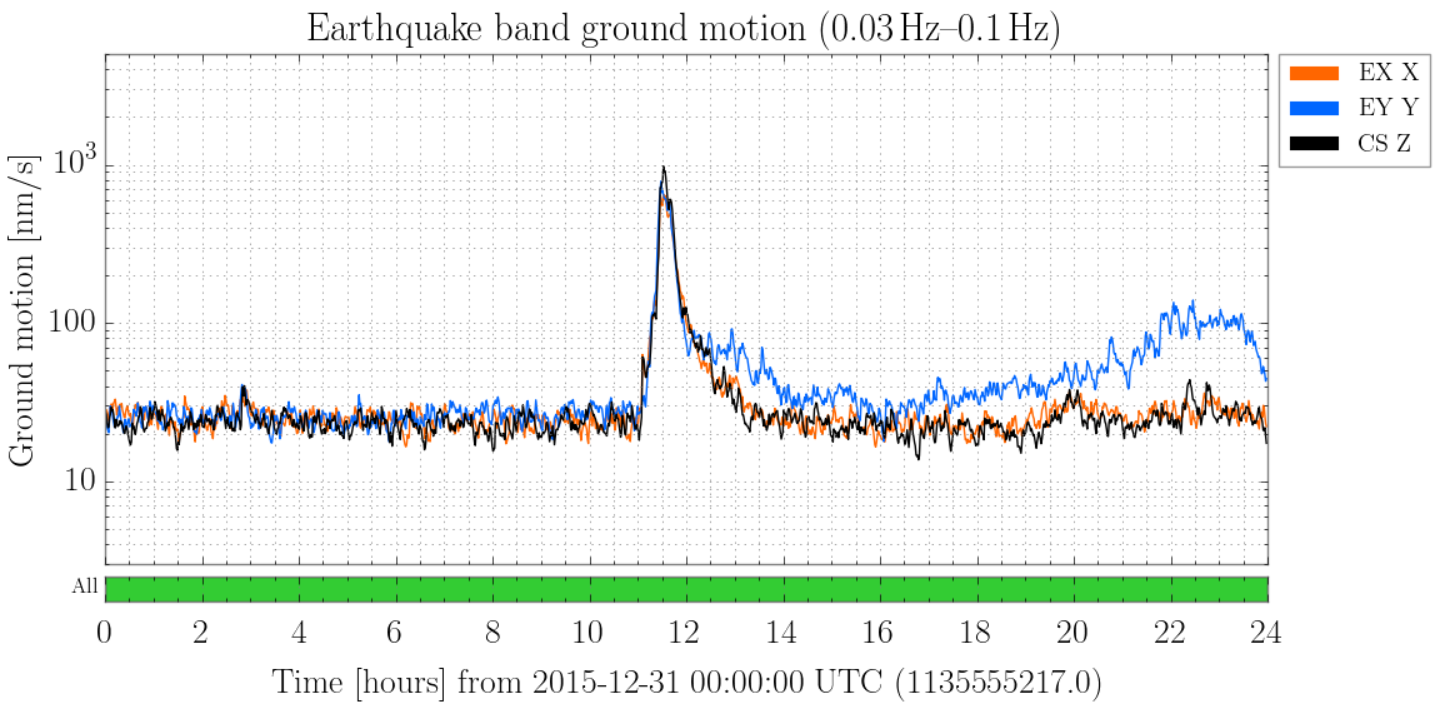
\includegraphics[width=\textwidth]{figures/EQ_band.png}
    \caption{Seismometer data showing a passing earthquake that knocked LHO out of lock during O1. Lock was lost at 11:23:14 UTC.}
    \label{fig:EQ_band}
\end{figure*}

Human activity around the site typically produces motion in the ``anthropogenic band" of 1\,-\,3\,Hz. Naturally this noise varies significantly with the time of day. Winds greater than about 20\,mph can affect the detector's output with most related seismic noise showing up between 0.5\,-\,15\,Hz. Wind can also affect building tilt at low frequencies. Vehicle traffic on nearby highways produces ground motion in the 2\,-\,15\,Hz band. This noise was reduced at LHO by a factor 2 by repaving the main highway next to the site~\cite{ana_pem}. Each site also has its own local noise sources such as pumps, fans, and air conditioning systems. When a local noise source cannot be removed, it is mitigated as much as possible via isolation systems.

Seismic injections are performed with a weighted cart and shaker. The shaker can be moved to different locations and used to inject ground motion at a desired frequency. A different power source is used for the injection equipment with respect to the detector electronics so that current draws won't couple through. In general the injections are performed at an equal distance to the witness sensor and assumed coupling site. 

\subsection{Acoustic}

Known sources of acoustic noise include: electronics fans (above 50\,Hz), chillers (below 60\,Hz), building air control (below 100\,Hz), thermally induced building creeks and thumps (broadband), nearby vehicles (50\,-\,150\,Hz), wind (broadband), and propeller driven aircraft (50\,-\,100\,Hz)~\cite{ana_pem}. Most in-vacuum electronics are well-isolated from sound waves, but several non-vacuum auxiliary systems, such as optical tables, have been found to be significant sources of acoustic coupling. All out of vacuum optical tables have therefore been acoustically insulated with enclosures to minimize the propagation of sound waves.

Acoustic noise couples to the GW strain channel primarily through beam jitter, beam clipping, and beam scattering. Sound waves drive the motion of optical mounts which results in modulations of the primary and auxiliary photodiode signals. Measures have been taken to reduce scattering, such as checking all optical surfaces for stray beams, using beam dumps for all stray light, removing unnecessary protection windows from photodiodes to prevent sensor prompt-reflection backscatter, and using damped material on optical mounts~\cite{ana_pem}.

Acoustic injections are performed with a large 500\,W speaker. This speaker is rolled around to different locations and used to inject loud signals. Acoustic coupling is generally higher in the corner station as opposed to the end stations due to the increased number of optical tables. Figure~\ref{fig:coupling} shows example coupling factors.

\subsection{Electromagnetic}

\begin{figure*}[t]
    \centering
    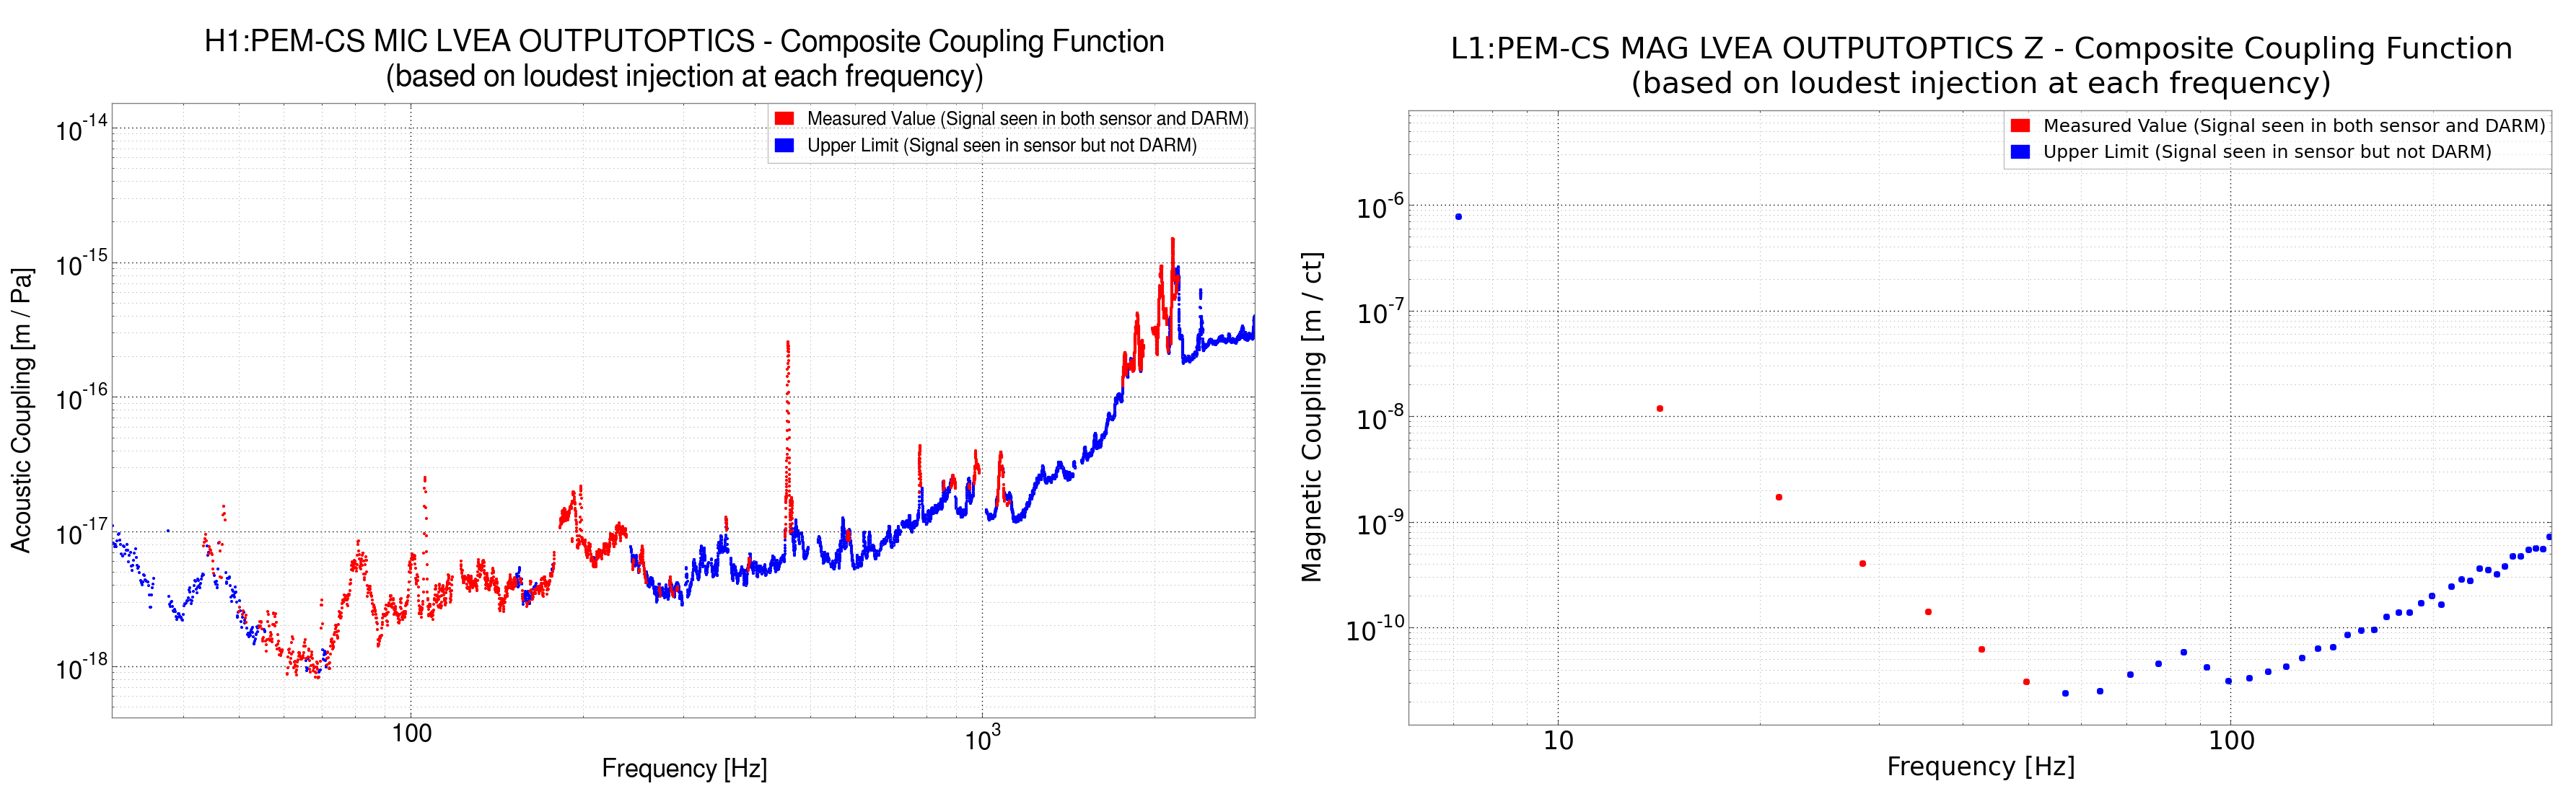
\includegraphics[width=\textwidth]{figures/coupling_factors.png}
    \caption{Left: Coupling factors for a microphone at LHO. Right: Coupling factors for a magnetometer at LLO. Blue data points are upper bound calculations because the injection was not visible in the GW strain channel. Both plots taken from PEM website~\cite{pem_website}.}
    \label{fig:coupling}
\end{figure*}

The LIGO detectors contain a large number of electronics, all of which produce electromagnetic fields. Motors, lights, computers, and building heaters are all examples of potential noise sources. Subtle issues such as flashing lights or significant draws of power can sometimes affect the detector. A refrigerator accidentally left plugged in at a Hanford end station caused mysterious issues for months during O1. PEM magnetometers are located around important electronics to monitor the fields and observe unusual behavior. The GW strain data contains a large 60\,Hz peak due to AC power lines. This peak can hurt LIGO's sensitivity to signals in its vicinity.

Electromagnetic noise couples to the detector primarily through electronic modules, cables, and magnets located on the interferometer optics. Each optic has five magnets, four on its back and one on its side, which are then actuated by coils mounted on the surrounding frame. Uniform magnetic field gradients do not have a direct displacement effect on the optic because the magnets alternate in polarity, however magnetic field gradients comparable to the magnetic field produced by the actuation coil can induce noise in the GW strain channel~\cite{ana_pem}.

Previous versions of the LIGO detectors were hindered by environmental radio frequency (RF) noise. This is because LIGO used a modulation-demodulation scheme (heterodyning) to generate error signals for controlling the length and angular degrees of freedom of the interferometer. Environmental RF noise coupled to the modulation frequencies and produced noise in the strain channel. Before S6, a DC homodyne scheme was adopted to reduce this coupling~\cite{fricke2012dc}. The current Advanced LIGO detectors continue to monitor environmental RF signals at 9 and 45\,MHz, two frequencies of interest for the control systems.

Magnetic injections are performed with a 1\,m (diameter) 100-turn copper coil. This coil is attached to a power source and can be wheeled around the site. The coil is typically located an equal distance from the magnetometer and the coupling site (magnet actuators on the optics). The strain contribution from ambient magnetic fields is usually well below LIGO's noise curve. Example magnetic coupling factors can be seen in Figure~\ref{fig:coupling}. RF injections are performed with an RF source located well outside of the corner station building and are done at the modulation frequencies of LIGO's control systems.

\section{System Installation}

Both LIGO sites underwent large-scale modifications after S6 in preparation for Advanced LIGO. A small number of PEM sensors were able to remain in place throughout the transition but the vast majority had to be removed for hardware upgrades. After the upgrades were complete, the PEM system had to be reinstalled. This installation process was performed over the course of two summers primarily by Robert Schofield, Anamaria Effler, Terra Hardwick, and myself.

Each sensor needs to be located very specifically in order to produce useful, clean data. Microphones are hung away from metallic surfaces to reduce echo and ambient noise. Magnetometers are placed next to specific electronics and must be oriented such that each dimension is properly monitored. Tiltmeters, seismometers, and infrasound microphones are located on the floor outside of vacuum chambers but must be clearly marked and out of the way for site workers. Accelerometers are mostly located in specific locations on the outside of vacuum chambers. They are also attached via epoxy to an insulating surface which is then attached via epoxy to the chamber wall. Other sensors were more difficult to install, such as the accelerometers in the Primary Stabilizing Laser (PSL) room and the RF antennae. The PSL is in a clean room that requires multiple stages of preparation along with specific attire to enter. The accelerometers were then carefully placed on optics tables. The RF antennae had to be installed along the ceiling in the electronics bay and above the corner station vacuum chambers. This required holes to be drilled in the walls while on top of very tall ladders. A two person rope system was then used to run the cable along the ceiling 

All of these sensors and their specific locations are mapped on the PEM website~\cite{pem_website}. As each sensor was installed, its information was put online for future reference along with a photograph of the installed sensor and an example data plot. The example data plots show typical power spectra for ambient noise. The exact location of each sensor was also calculated via trilateration using a laser distance measure and certain precisely measured spots on the floor (used for site construction). These precise coordinates are also on the website and can be theoretically used to calculate the velocity of a propagating wave or the epicenter of an observed disturbance. Figure~\ref{fig:pem_website} shows an example screenshot from the PEM website.

\begin{figure*}[t]
    \centering
    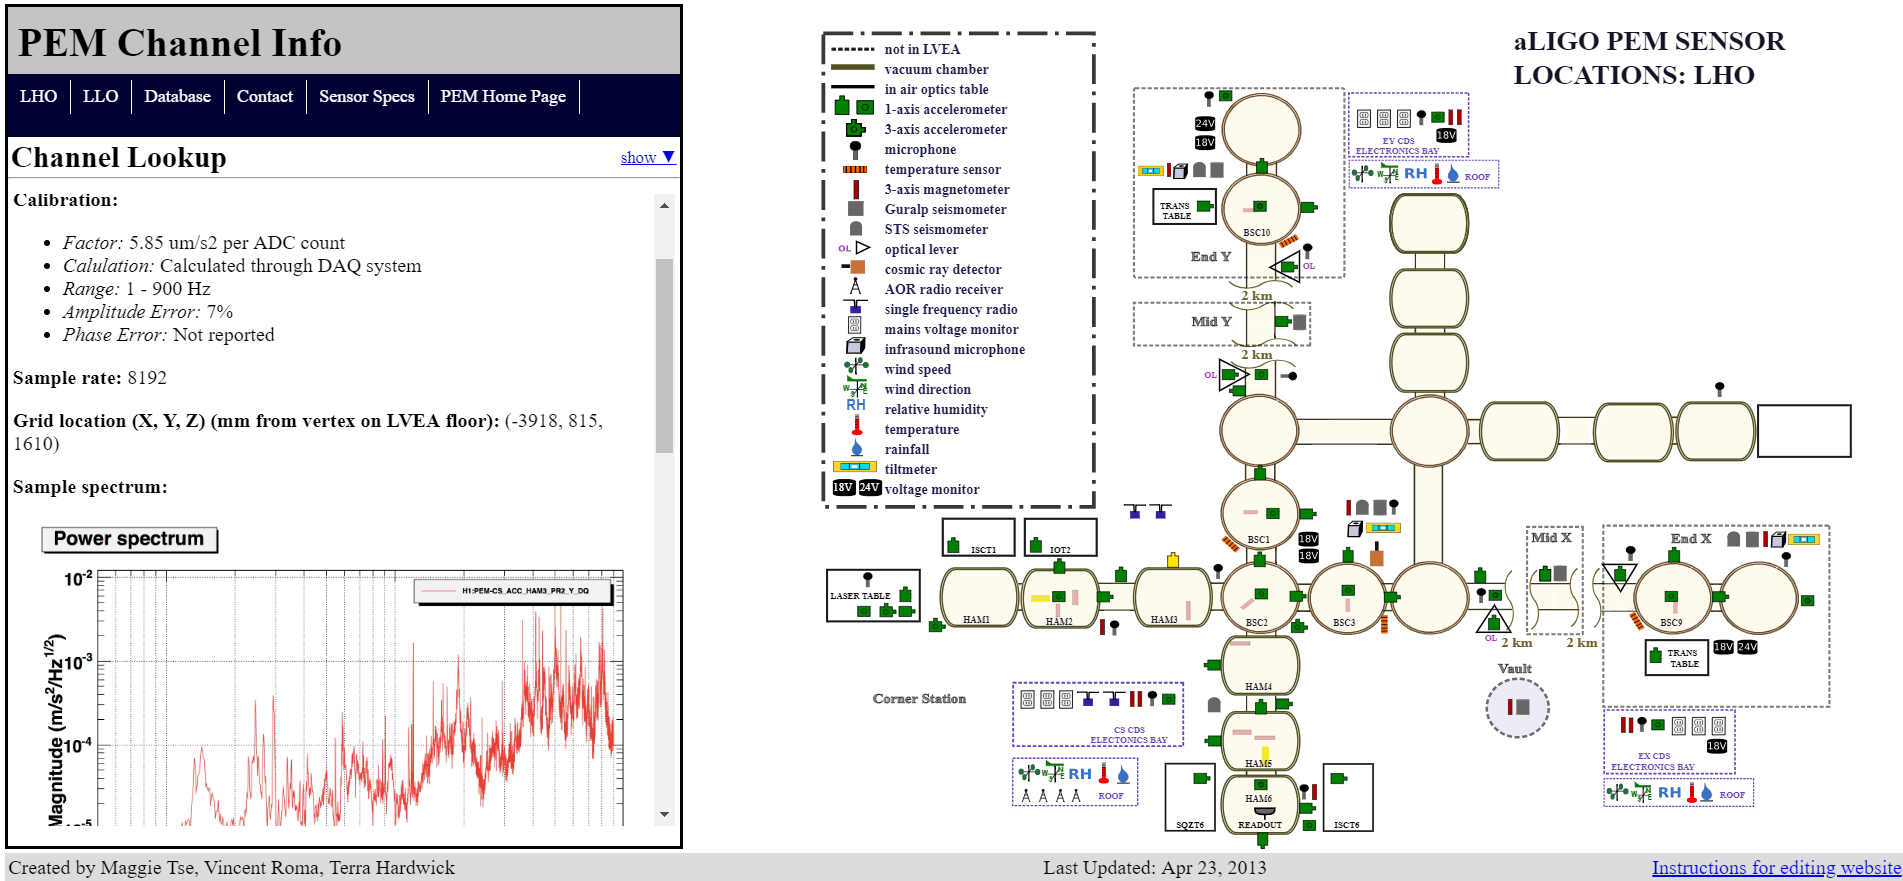
\includegraphics[width=\textwidth]{figures/pem_website.png}
    \caption{Screenshot from the PEM website~\cite{pem_website}. Sensor map on the right is interactive. Clicking on a sensor brings up its hardware information, calibration information, coordinates, example power spectra, and installation photo.}
    \label{fig:pem_website}
\end{figure*}

In addition to installing each sensor, the sensors need to be powered and their data needs to enter LIGO's Data Acquisition System (DAQ). This means that cables had to be ran from the electronics bay out onto the floor. These cables leave the electronics bay and enter the site floor via elevated cable trays above the vacuum chambers. Sometimes these cables must be ran for hundreds of feet, passing along the floor underneath hardware and/or above vacuum chambers 12 feet off the ground. Properly running long cables from the electronics bay to sensors out on the floor requires at least two people and can take hours. After everything is properly installed, the system must be tested. Some sensors simply don't behave properly and must be replaced. The accelerometers are connected to a power supply in the electronics bay which then sends the signal to an Analog-to-Digital Converter (ADC). Some of these older power supplies suffered from significant ``crosstalk", where one accelerometer's signal would cross over into the data of a nearby channel. After extensive testing, these bad channels were avoided and some of the power supplies had to be replaced. All of these cable connections for the PEM system also had to be mapped and documented in the electronics bay. After working with Robert Schofield to install the PEM system at Hanford, Terra Hardwick and I spent the next summer in Livingston installing that PEM system with Anamaria Effler.

The status of PEM sensors is monitored with an algorithm called LigoCAM. LigoCAM was created by Dipongkar Talukder and is accessible from the PEM website~\cite{pem_website}. This algorithm monitors the band-limited root-mean-square (BLRMS) of every PEM sensor to determine when a sensor has come unplugged or has experienced a significant change of state. Students working on site, such as myself, helped to develop and tweak the settings of LigoCAM in order to make it operate as planned. This algorithm continues to run and notifies workers when PEM sensors change state unexpectedly.

\section{Detection Vetting and GW150914}

The LIGO interferometers measure distance more precisely than any device in history. This makes the interferometers incredibly sensitive to environmental effects and hardware glitches. In order to claim an observation of a GW signal, LIGO must be able to guarantee that their signal is extraterrestrial in origin. This was all the more important for the first direct GW observation, GW150914, as previous researchers have incorrectly claimed GW detections in the past~\cite{weber1969evidence}. This section will summarize the PEM detection vetting process with a focus on GW150914. A brief summary of the PEM report is included in the detection paper~\cite{GW150914} and members of the LIGO collaboration can view the full PEM report in the event log~\cite{pem_GW150914}.

The primary concern for a PEM vetting report is whether or not an environmental source could have caused the GW signal. GW150914 was detected at 09:50:45 UTC by both LIGO detectors. At that time, 13-15\% of PEM sensors were inactive or had not yet been fully installed. GW150914 surprised everyone at the tail end of an engineering run, right before the data-taking period was scheduled to begin. Fortunately, sensor redundancy provided good coverage despite the missing channels. Multiple magnetometers were inactive at both sites, but all of those locations had at least one functioning magnetometer. There were plenty of functioning accelerometers and seismometers throughout both sites to ensure that significant ground motion could not go undetected. Every missing channel is listed in the report and its effect on coverage is analyzed. The most important missing channels were the mains voltage monitors at LLO, but voltage glitches also produce magnetic glitches and magnetometers were functioning. In short, both detectors had sufficient coverage to observe environmental influences.

\begin{figure*}[t]
    \centering
    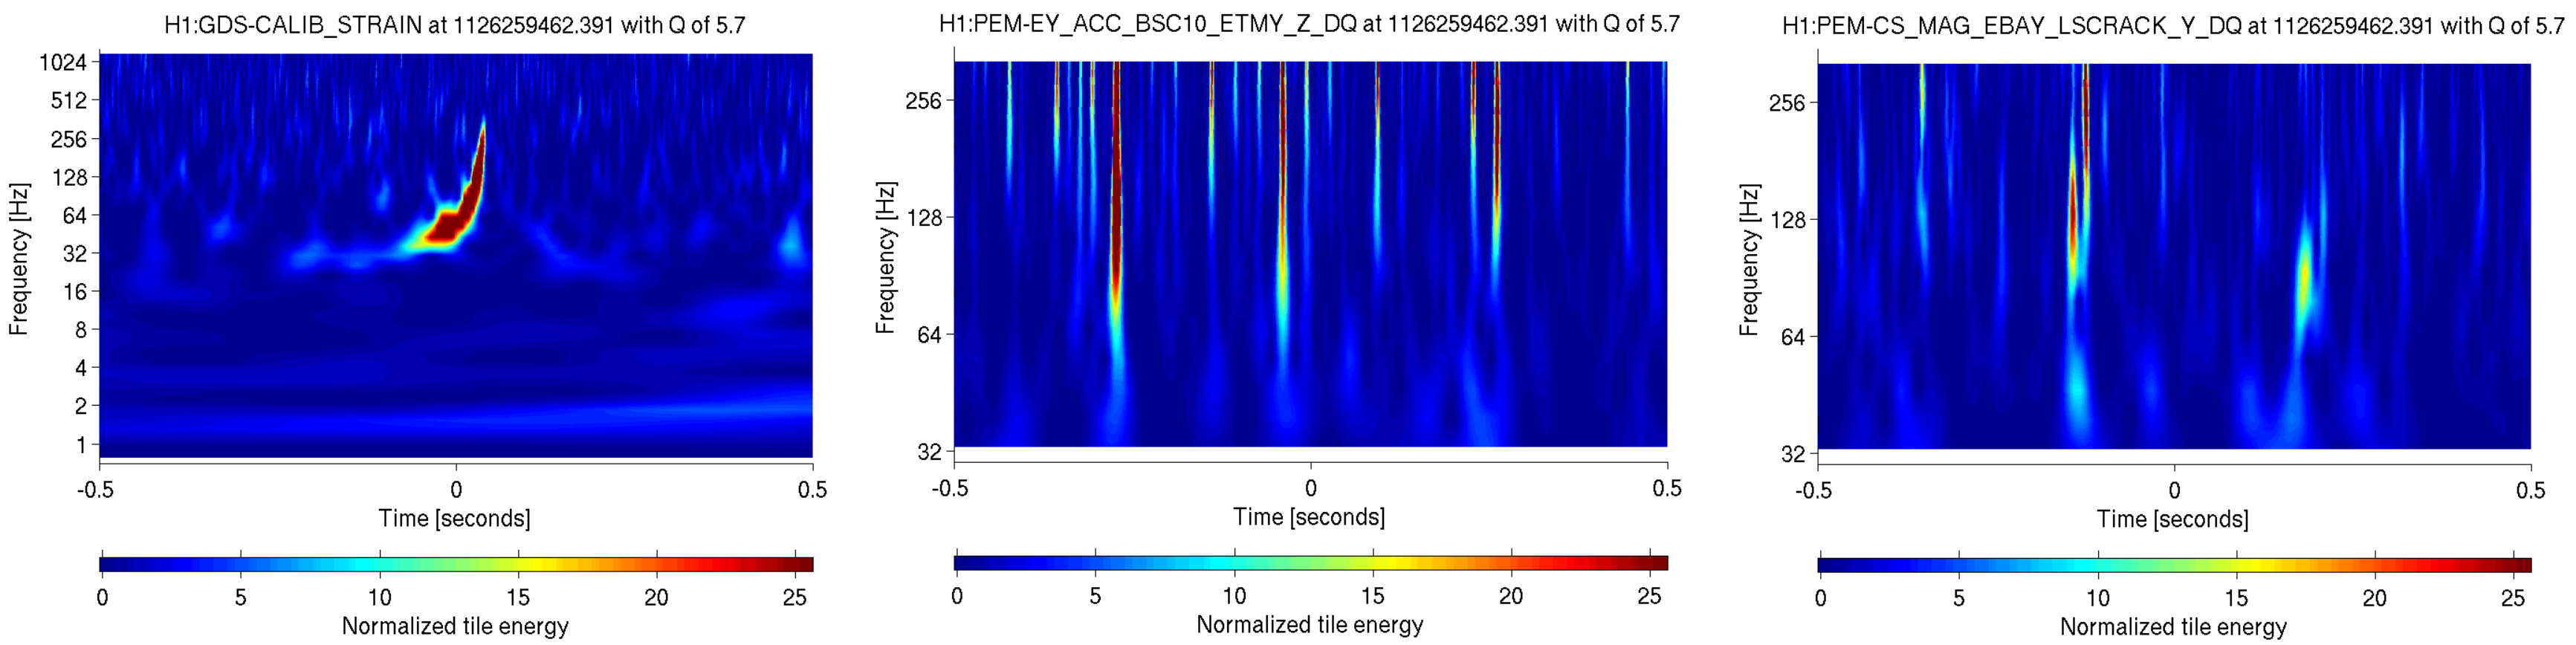
\includegraphics[width=\textwidth]{figures/wdq_plots.png}
    \caption{Omega scan plots from LHO. Left: GW strain channel. Center: Accelerometer on corner station vacuum chamber. Right: Magnetometer in corner station electronics bay. No PEM channels had a time-frequency path similar to the GW signal.}
    \label{fig:wdq_plots}
\end{figure*}

An Omega scan~\cite{chatterji2004multiresolution} is a commonly used spectrogram tool for looking at signals and glitches in LIGO data. Spectrograms are produced for the GW strain channel and any other channels that show increased activity during the event time. Omega scans were ran on every PEM channel for the frequency band 30\,-\,350\,Hz at both sites. This frequency band was chosen because of the time-frequency (TF) path of the signal. Some PEM channels had sufficient noise to produce plots in the Omega scan, but none of them had a TF path similar to the GW observation. Figure~\ref{fig:wdq_plots} shows Omega scan plots of the GW150914 signal and two PEM sensors at LHO. As described earlier in this section, coupling factors can be calculated for PEM sensors that describe how noise sources influence the strain channel. This can be done in terms of amplitude or in terms of SNR. In both cases, the coupling relates the PEM sensor signal to the GW strain signal. SNR coupling factors were used for each PEM sensor in the Omega scan to calculate how loud the signal would have to be to generate the observed strain signal. This was done for all sensors, regardless of TF path. The loudest environmental signal at LHO would have had to have been 31 times louder in order to produce the strain SNR. The loudest environmental signal at LLO would have had to have been 23 times louder~\cite{pem_GW150914}.

In addition to the Omega scans, power spectra were produced for every PEM sensor around the time of the event. Two plots were created, one with 1 second of data, and the other with 64 seconds of data. Spectra for every single PEM channel was plotted against its background levels. Any channels showing unusual noise around the event time were further investigated. No significant concerns were found and Figure~\ref{fig:spectra_plots} shows some example spectra plots for PEM sensors. Spreadsheets with all of the channel information and links to plots were included in the PEM vetting report~\cite{pem_GW150914}. All PEM sensors were checked for abnormal behavior through multiple means, and none showed evidence of an environmental disturbance that could have caused GW150914.

\begin{figure*}[t]
    \centering
    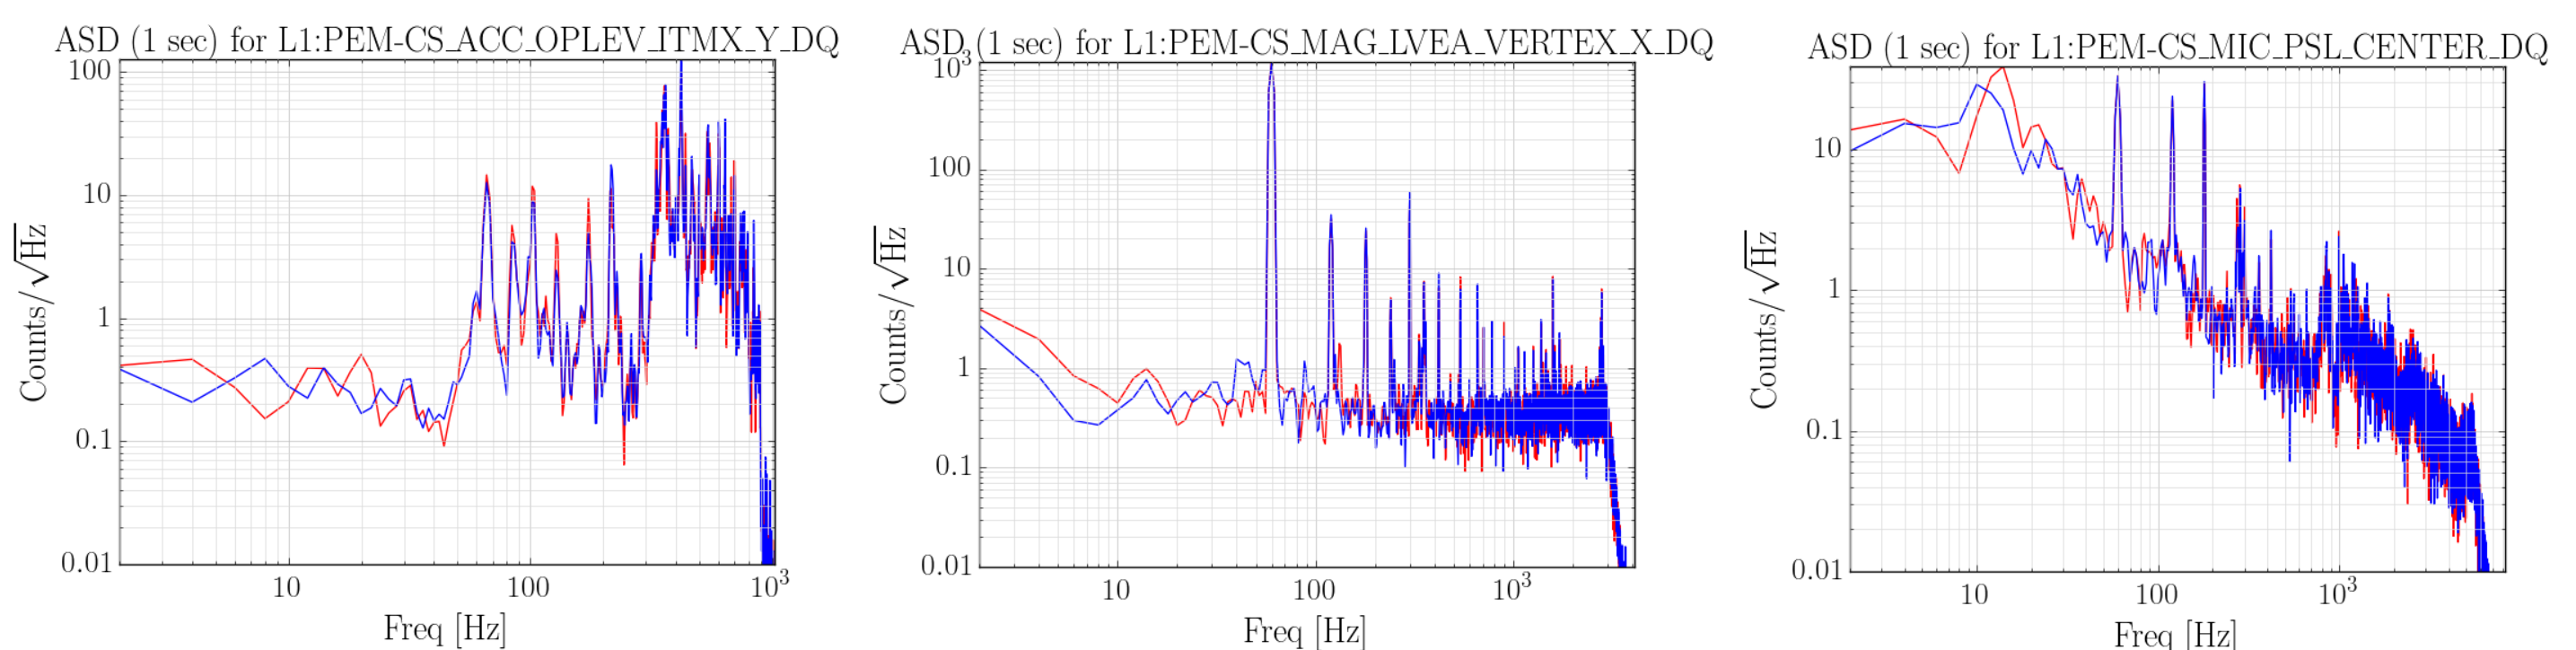
\includegraphics[width=\textwidth]{figures/spectra_plots.png}
    \caption{Spectra plots for three LLO PEM sensors. Left: Accelerometer on optical lever. Center: Magnetometer in corner station. Right: Microphone in PSL room. Plots contain one second of data centered on GW150914 event time. Red trace represents spectra from the event time, blue trace is a reference from 100 seconds before.}
    \label{fig:spectra_plots}
\end{figure*}

It is possible, through upconversion or downconversion, for noise outside of our frequency band of interest to contribute to the observed GW strain signal. One noteworthy mechanism of downconversion is addressed in the PEM report. Non-linear coupling at HAM6 (both sites), produced by intermodulation of the vibration frequency and the OMC length dither (4100 Hz at LHO), can down-convert vibration above 2500\,Hz into the 30-350\,Hz event band~\cite{pem_GW150914}. However, none of the microphones or accelerometers around HAM6 showed any high frequency noise above background levels, indicating that there was no high frequency noise to down-convert. It is also highly unlikely that upconverted or downconverted noise would resemble the transient, chirp-like signal seen in GW150914.

The environment can influence LIGO interferometers through physical contact, electromagnetic waves, static and electric magnetic fields, and possibly high-energy radiation. Environmental influences that propagate near the velocity of gravitational waves and could influence both sites must be monitored. Global-scale high energy radiation events and electromagnetic events are considered, potentially including power grid events~\cite{pem_GW150914}. The Hanford site has a cosmic ray detector located underneath a vacuum chamber. Cosmic rays are unlikely to produce non-random coincidences between detector sites and the cosmic ray environment was quiet around the event time. Certain hardware at both detector sites is synchronized to GPS time, which can produce low-amplitude combs of spectral lines that are coherent between sites. However, there is no reason to expect transient data corruption events that are synchronized between sites. Such events would be also be simultaneous, as opposed to our observed signal which has a reasonable light speed delay between the two detectors. Solar events would be detected by the RF receivers if they were significant enough to affect the strain channel. Solar radio flares would have been blocked (it was night time) and there were no flares around the event time. There were no coronal mass ejection geomagnetic storms. If seismic or acoustic noise happened coincidentally at both sites then it would have been detected by PEM sensors.

The global electromagnetic environment is always examined around a GW event. Generally, any electromagnetic or RF signal that was strong enough to affect the GW strain channel would be detected by the PEM magnetometers, however, data from external electromagnetic and RF observatories is always reviewed. No significant local electromagnetic or RF events were observed around GW150914. Schumann resonances are a lightning driven comb of peaks with the fundamental at about 8\,Hz (given by light travel time around the earth). They do not show up strongly in the event data and there's no reason to believe they would produce the transient GW signal observed. There was a large burst of lightning in Burkina Faso right around the event time that caused some concern, however calculations showed that at that distance it was at least three orders of magnitude too small to create the GW signal. Lightning strikes also release their energy in a broadband fashion, as opposed to the observed chirp. There were many closer lightning strikes that day, none of which affected the detectors.

None of the PEM sensors produced any evidence that an environmental source could have caused GW150914. Data from many external observatories reinforced this conclusion. The PEM vetting process has been streamlined over time as more GW observations have been recorded. Spectra are no longer produced for every PEM channel and the Omega scan process has been greatly improved. The PEM vetting is moving towards full automation, which will be necessary as the LIGO detectors improve their sensitivity. Eventually, GWs from binaries will be observed weekly or daily, requiring a very efficient vetting process.

\section{Noise Correlation Analysis Tool}

During S5 and S6, seismic uponversion was a significant problem for the LIGO detectors. Upconversion refers to low frequency noise that causes higher frequency noise in the strain channel. Upconversion can happen through different mechanisms, sometimes ones that are not obvious. In S5 and S6, microseismic noise (0.1\,-\,0.3\,Hz) caused upconversion due to the Barkhausen effect. The Barkhausen effect refers to suddenly changing magnetic domains in a ferromagnet due to a changing external field. This happened either in the test mass magnets themselves or in the magnetic parts associated with the actuation on the mirrors~\cite{S6_characterization, weiss2008various}. Essentially, something was ferromagnetic that shouldn't have been. These issues lead to the development of software to help find and identify upconversion.

The Noise Correlation Analysis Tool (NCAT) was originally developed by Ryan Quitzow-James. This algorithm compared the band-limited root-mean-square (BLRMS) of a PEM channel to the BLRMS of the GW strain channel in order to find correlated noise bands. The mechanism at play behind this noise correlation is irrelevant. This allowed microseismic noise in seismometers to be correlated to the higher frequency (20\,-\,400\,Hz) strain noise. Each time the code is ran, a set of PEM channels and frequency bands can be chosen. All channels and frequency bands are then searched for correlated noise and a simple web page is produced to display the results. I took over this code and project as my first foray into coding and LIGO-related science. The code was rewritten entirely in Python (previously the BLRMS calculations used a C executable) for simplicity and also to incorporate GWpy, a library of GW-related Python functions. From that point, the math and figure of merit calculations continued to be expanded upon.

NCAT was designed to be ran on large spans of data, sometimes months. The data, for both PEM sensors and GW strain, is then broken up into variable sized sections (usually 16 or 32 seconds long). A one-sided power spectral density (PSD) is calculated for these sections of data which is then used to calculate the BLRMS in the usual way,
\begin{equation}
\label{equ:blrms}
    \text{BLRMS} = \sqrt{\sum_{f=f_{1}}^{f_{2}} \text{PSD}(f) df}
\end{equation}
where $f_{2}$ and $f_{1}$ represent the upper and lower frequency bounds respectively. The formula has been written as a sum instead of an integral because the data is discrete. Once all of the BLRMS calculations have been performed, the data can be plotted and figures of merit can be calculated.

\begin{figure*}[b!]
    \centering
    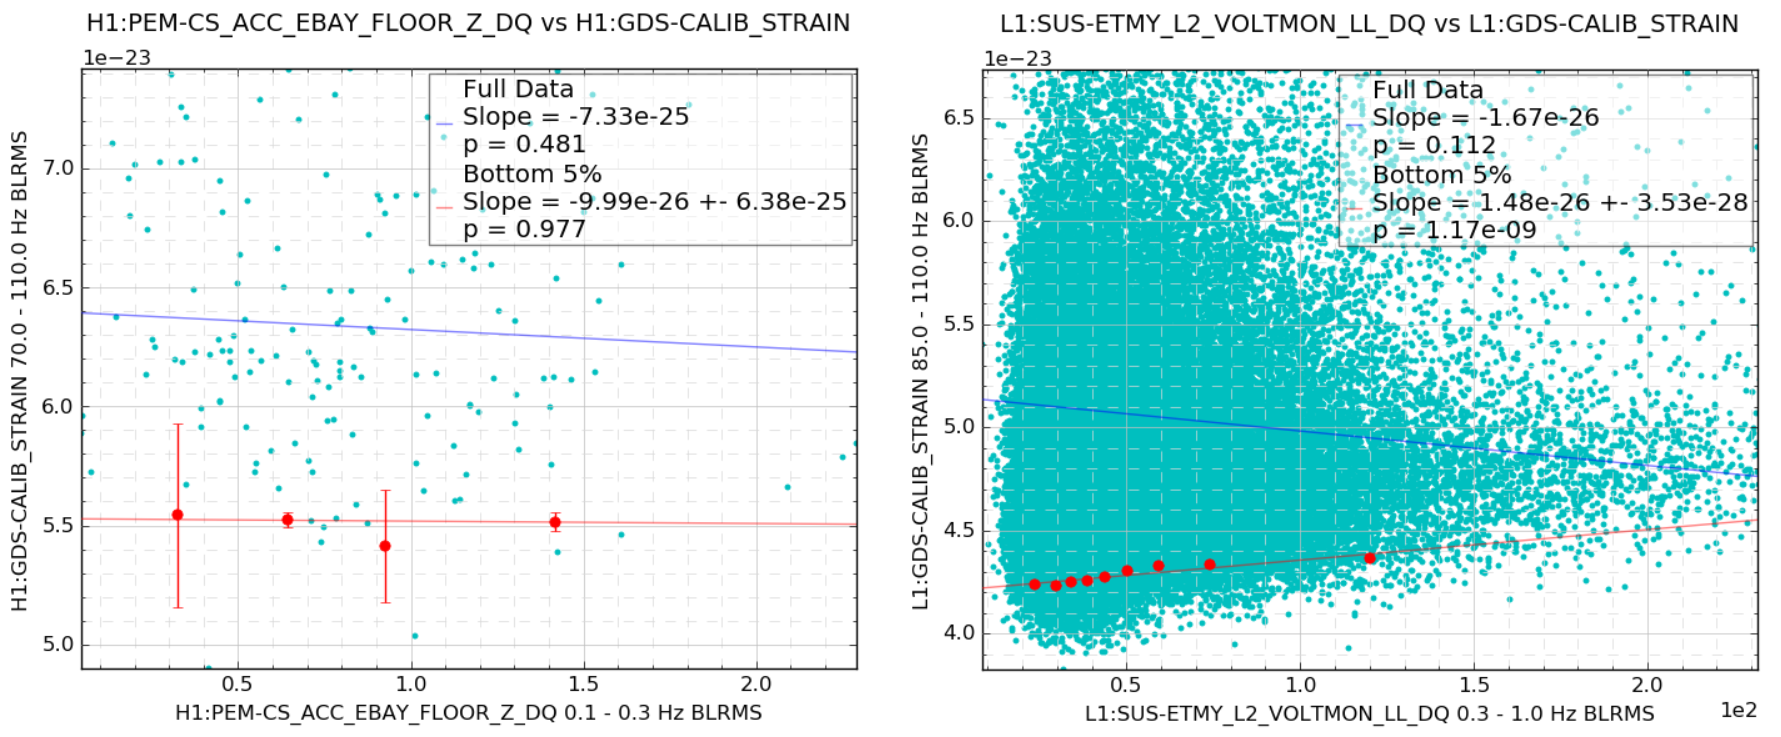
\includegraphics[width=\textwidth]{figures/ncat_plots.png}
    \caption{Example NCAT plots showing low frequency BLRMS for PEM sensors vs higher frequency BLRMS for strain. Left plot shows no evidence of correlated noise with a p-value of 0.977 (bottom 5\%). Right plot shows strong evidence with a p-value of $1.17\times10^{-9}$.}
    \label{fig:ncat_plots}
\end{figure*}

Figure~\ref{fig:ncat_plots} shows two example NCAT plots with BLRMS data. The PEM sensor data is plotted along the x-axis and the GW strain data is plotted along the y-axis. The code is searching for a correlation between these two frequency bands, but the GW strain channel has many noise sources all contributing to its overall signal. For that reason, the quietest strain data points are more useful as they will give a more accurate relationship between the two frequency bands, less corrupted by other noise sources. All of the blue data points are binned horizontally to create the red data points. The binning function is flexible and ensures that each bin has sufficient data points. This is visible in the right plot as the rightmost bin (red data point) is located a significant distance from its nearest neighbor. This is due to the smaller number of data points in this region. The red data points represent the mean of the bottom 5\% (optional) of each bin. When there are sufficient data points the bottom 1\% can be used. Each red data point has error bars based on the standard deviation of the data points used in its calculation. A linear best fit line is then calculated for the red data points. If this line has a significant positive slope, then the two noise bands are correlated. The significance of the slope is determined with a t-test, which results in a p-value for our figure of merit. These statistics are visible in the legend of each plot, for the full data (blue) and bottom 5\% (red).

The linear fit line is calculated using standard formulas, but weights each data point by the inverse square of its standard error (error bars). Data points with large errors will affect the linear fit less significantly. All formulas can be found in numerous statistics textbooks~\cite{freedman2007statistics, stats_shao}. For a series of data points with x and y values, the y-intercept is,
\begin{equation}
\label{equ:y_intercept}
    \text{y-intercept} = \frac{\big(\sum \frac{x_{i}}{e_{i}^{2}}\big) \big(\sum \frac{x_{i}y_{i}}{e_{i}^{2}}\big)-\big(\sum \frac{y_{i}}{e_{i}^{2}}\big) \big(\sum \frac{x_{i}^{2}}{e_{i}^{2}}\big)}{\big(\sum \frac{x_{i}}{e_{i}^{2}}\big)^{2} - \big(\sum \frac{x_{i}^{2}}{e_{i}^{2}}\big) \big(\sum \frac{1}{e_{i}^{2}}\big)}
\end{equation}
where $e_{i}$ represents the standard error  of each data point (error bars in plot). The slope is found similarly as,
\begin{equation}
\label{equ:slope}
    \text{slope} = \frac{\big(\sum \frac{x_{i}}{e_{i}^{2}}\big) \big(\sum \frac{y_{i}}{e_{i}^{2}}\big)-\big(\sum \frac{x_{i}y_{i}}{e_{i}^{2}}\big) \big(\sum \frac{1}{e_{i}^{2}}\big)}{\big(\sum \frac{x_{i}}{e_{i}^{2}}\big)^{2} - \big(\sum \frac{x_{i}^{2}}{e_{i}^{2}}\big) \big(\sum \frac{1}{e_{i}^{2}}\big)}
\end{equation}
with the standard error of the slope (SE) given by,
\begin{equation}
\label{equ:slope_error}
    \text{SE} = \sqrt{\frac{\sum \frac{1}{e_{i}^{2}}}{\big(\sum \frac{x_{i}^{2}}{e_{i}^{2}}\big) \big(\sum \frac{1}{e_{i}^{2}}\big)-\big(\sum \frac{x_{i}}{e_{i}^{2}}\big)^{2}}}
\end{equation}
This standard error of the slope is used directly in our t-test, where our t statistic is defined as~\cite{freedman2007statistics},
\begin{equation}
\label{equ:t_test}
    \text{t} = \frac{\text{slope}}{\text{SE}}
\end{equation}
This value can be converted to a p-value using the cumulative distribution function~(cdf) for a Student's t distribution. Explicitly,
\begin{equation}
\label{equ:p_value}
    \text{p-value} = 2\cdot\text{cdf}(-|\text{t}|)
\end{equation}
This p-value represents the probability of obtaining a slope that deviates from zero by more than the slope of the best fit line, if a slope of zero is the true relationship between the x and y variables. Equivalently, it is the probability of obtaining a t statistic that deviates from zero by more than the calculated t value. The left plot in Figure~\ref{fig:ncat_plots} has a p-value of 0.977 (bottom 5\%) and shows no evidence of upconversion, while the right plot has a p-value of $1.17\times10^{-9}$ and shows strong evidence. The NCAT results are ranked by these p-values on the final display page.

NCAT was used to find upconversion during O1, O2, and the engineering runs that preceded them. During ER7, microseismic (0.1\,-\,0.3\,Hz) noise and anthropogenic noise (1\,-\,10\,Hz) upconverted into strain noise (130\,-\,400\,Hz) at LHO. This noise was witnessed by seismometers and suspension channels. Similar upconversion was present at LLO for 1\,-\,10\,Hz and there was also a strong correlation between the 0.1\,-\,0.3\,Hz band of ground motion and the 55\,-\,65\,Hz band of strain, probably indicating that motion around the microseismic peak was intermodulating with motion around 60 Hz, producing sidebands. A summary of results was posted in LHO log 19220. Microseismic upconversion continued throughout O1 and affected the strain bands of 55\,-\,65\,Hz, 85\,-\,110\,Hz, and 50\,-\,200\,Hz. Higher frequency environmental noise between 30\,-\,50\,Hz was found to correlate with strain noise in the bands of 85\,-\,110\,Hz, 121\,-\,200\,Hz, and 1000\,-\,2000\,Hz. There was some concern about noise in the 700\,-\,900\,Hz and 700\,-\,1200\,Hz bands potentially downconverting into strain, but no evidence for this was found. These results are online in LHO log 23658. During O2, higher frequency upconversion from the bands of 20\,-\,30\,Hz, 33\,-\,43\,Hz and 43\,-\,59\,Hz was seen to influence strain bands of 86\,-\,130\,Hz and 130\,-\,170\,Hz. Over time, seismic upconversion has become less of a debilitating problem for the LIGO detectors, primarily due to the improved active seismic isolation. Other advancements, such as offline noise removal through a Wiener filter and witness sensor, have helped to further mitigate the problem of environmental noise and upconversion.

\section{Glitch and Line Hunting}

Glitches are transient noise artifacts in LIGO's data. These can originate from hardware or software and can be extremely difficult to track down. ``Blip" glitches have been present in all Advanced LIGO data and are still mysterious heading into O3~\cite{cabero2019blip}. Glitches contaminate brief periods of detector data and can possibly be mistaken for GW observations. This, along with greatly improved sky localization, is why it's necessary to operate multiple LIGO detectors simultaneously. Lines refer to narrow peaks in spectra and are caused by continuous noise sources. Lines can hurt the sensitivity of a detector and greatly hinder the search for continuous waves in LIGO data. Finding and removing sources of lines and glitches is an important aspect of PEM work. The rest of this section will summarize two example cases.

\begin{figure*}[b!]
    \centering
    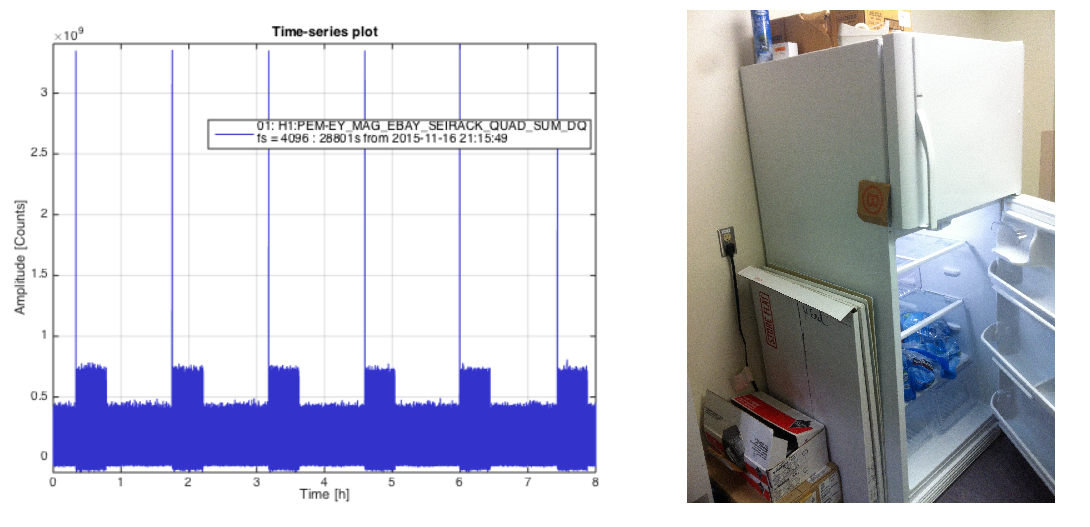
\includegraphics[width=\textwidth]{figures/fridge_plot.png}
    \caption{Left: Magnetometer plot at EY during O1 showing periodic glitches followed by temporarily elevated fields. Right: The culprit.}
    \label{fig:fridge_plot}
\end{figure*}

Periodic glitches centered around 60\,Hz occurred throughout all of O1 at LHO. Approximately once per hour a loud 60\,Hz glitch would be accompanied by increased magnetic fields at the Y end station (EY). This small magnetic field would disappear on the order of minutes and can be seen in Figure~\ref{fig:fridge_plot}. The period between glitches seemed to be slowly increasing over time. There was also a regular burst of glitches every Tuesday morning, which is maintenance day on site. These glitches appeared to be related to the use of electronics at EY, but the actual source avoided detection for many months. Magnetometers in the electronics bay showed larger spikes and post-glitch fields than the magnetometers next to the vacuum chambers, suggesting the issue was in that room. Using magnetometers plugged into oscilloscopes for portability, Borja Sorazu and I examined the entire electronics bay. The different magnetometer axes had shown different strength fields after a glitch. Rotating the magnetometers confirmed that the observed fields were real and not a rack related issue. The only piece of equipment in the room with strong magnetic fields was the Endevco\textsuperscript{\textregistered} power supply, which powers the PEM accelerometers. This was also the only device plugged into AC power via the wall. Microphones in the electronics bay had picked up a small signal when the glitches occurred, but no sound was audible to human ears.

Eventually it was noticed that glitches occurred whenever someone used the shoe cleaner, or anything else that pulled significant AC current from the wall. This would explain why there was always a burst of glitches on Tuesday mornings as workers entered the building and cleaned their shoes. Almost by chance, it was noticed that a refrigerator in the corner of the end station was plugged in. This refrigerator was surrounded by unused equipment in a makeshift storage room near the electronics bay and was not supposed to be connected to power. Unplugging the refrigerator immediately stopped the periodic 60\,Hz glitches. This also explained why the period between glitches was slowly increasing. Glitches were occurring when the compressor in the refrigerator turned on. As the weather outside got colder, the refrigerator's temperature was increasing at a slower rate, increasing the period between glitches. After this was realized, the Endevco\textsuperscript{\textregistered} power supply was further tested as a potential coupling site for these glitches. Unfortunately no good evidence was found and the exact coupling mechanism behind these glitches was never definitively proven. Regardless, the glitches have been removed from LIGO data. A summary of this work can be viewed in LHO log 23483.

\begin{figure*}[t]
    \centering
    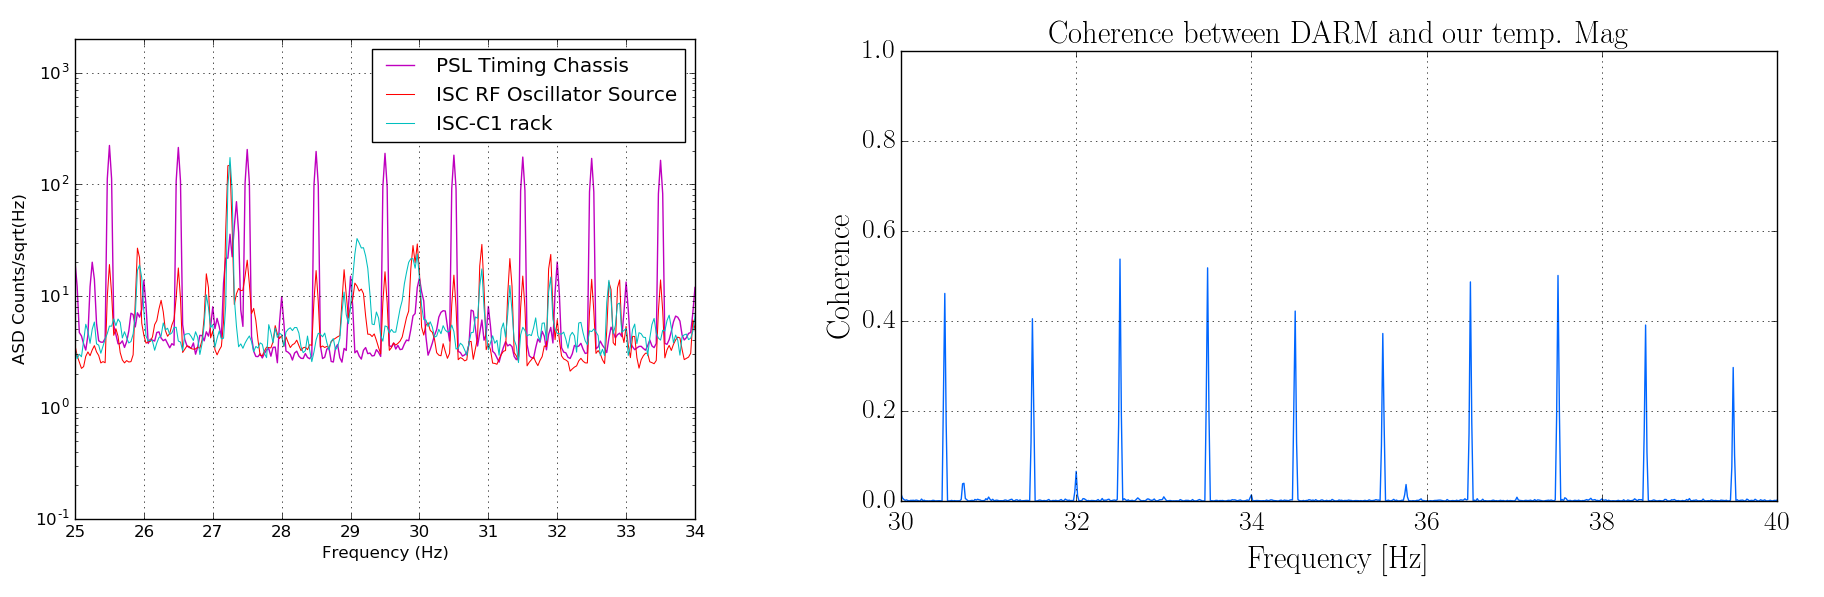
\includegraphics[width=\textwidth]{figures/LED_plots.png}
    \caption{Left: Magnetometer data from different locations at EY. Combs were strongest near timing equipment. Right: Coherence between temporary magnetometer and DARM (strain) confirming that this is the correct noise source.}
    \label{fig:LED_plots}
\end{figure*}

A strong comb with 1\,Hz spacing and 0.5\,Hz offset was also present in LIGO's data throughout O1. Several magnetometer channels at both end stations showed coherence with the strain channel. Once again portable magnetometers were used to investigate the end station with an emphasis on the electronics bay. The comb was clearly visible around nearly all electronics, but it was particularly strong around equipment associated with the timing system. Figure~\ref{fig:LED_plots} shows the combs in magnetometer data and coherence with the strain channel. The timing system contains master and slave components with LED indicators that draw power as a square wave with 2 second period. This would produce the observed comb in a Fourier series. Initially, the slave cards were placed on separate power supplies at the corner station and both end stations, however this did not reduce the strength of the comb. Replacing the power supply for the master system was considered, but ultimately it was decided to update the firmware to stop the LEDs from flashing. This did not completely remove the combs, but long term studies showed that the strength of the combs decreased by an order of magnitude. This work was published in the O1-O2 lines paper~\cite{covas2018identification}.





























\chapter{Core-Collapse Supernovae}
\label{chp:CCSNe}

Supernovae have been witnessed and recorded by humanity for thousands of years. As massively energetic explosions, they can shine brightly in the sky for weeks or months at a time. In 1934, Baade and Zwicky~\cite{baade1934remarks} famously proposed that supernovae might represent the transition of ordinary stars into neutron stars. Over 20 years later, Burbidge et al.~\cite{burbidge1957synthesis} suggested that supernovae might also be important for the synthesis and dissemination of heavy elements. By 1960, Hoyle \& Fowler~\cite{hoyle1960nucleosynthesis} had proposed that there were two main types of supernovae, one involving thermonuclear runaway in degenerate conditions (type Ia), and the other involving the implosion of a stellar core (types II, Ib/c, and hypernovae). The first type occurs when a white dwarf, typically in a binary system, accretes enough mass to reignite carbon fusion~\cite{chen2009progenitors}. This ``runaway nuclear fusion" completely disrupts the star, blowing it apart. This process is believed to be relatively isotropic with no significant asymmetries, and as such, is not expected to emit GWs. Core-Collapse Supernovae (CCSNe) on the other hand are expected to contain significant asymmetries and GW emission.

\begin{figure*}[t]
    \centering
    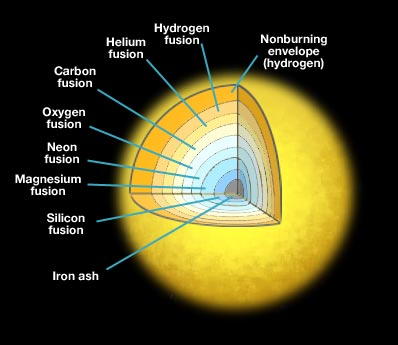
\includegraphics[width=4in]{figures/CCSN_strata.jpg}
    \caption{The stratified distribution of elements in a CCSN progenitor. Figure reproduced from~\cite{strata_source}.}
    \label{fig:CCSN_strata}
\end{figure*}

Near the end of a star's life ($8M_\odot$\,-\,$100M_\odot$~\cite{thesis_jade, janka}) its mass will be distributed by density, with heavier elements near the core and lighter elements composing an outer envelope. This situation is sometimes compared to the layers of an onion and can be seen in Figure~\ref{fig:CCSN_strata}. These stars have enormous gravitational binding energies of order $\sim\,10^{53}$\,ergs~\cite{colgate1966hydrodynamic}. Nuclear burning will cease when the core is composed of iron group nuclei (sometimes ONeMg) and the star becomes gravitationally unstable. When the core reaches the Chandrasekhar mass ($1.44M_\odot$) the electron degeneracy pressure will be overcome and collapse will begin. Eventually the inner core will reach nuclear density and the nuclear equation of state (EoS) will stiffen, causing a shock wave to rebound out radially from the just formed proto-neutron star (PNS). This shock wave will propagate outwards, losing energy via the disassociation of infalling matter and the emission of neutrinos through optically thin regions. The shock wave will quickly stall and become an accretion shock, which must be revived within $\sim$\,0.5\,-\,3 seconds to successfully explode and avoid transitioning directly to a black hole~\cite{thesis_jade}. This shock revival mechanism is still not completely understood and represents one of the biggest unknowns in astrophysics. Gravitational energy is primarily converted to neutrino emission during a CCSN and this offers a possible energy reservoir to revive the shock front. GWs, along with neutrinos, carry information directly from the core of a collapsing star, as opposed to electromagnetic radiation which is only emitted from the outer layers. This means that GWs and neutrinos offer the best opportunities to learn about the inner workings of a CCSN. Contemporary reviews of the CCSN process can be found from Janka~\cite{janka} and M\"uller~\cite{muller2016core}. Subsequent sections in this chapter will detail the core-collapse process, possible revival mechanisms, CCSN asymmetries, detection prospects, and the current state of simulations.

\section{Paths to Core Collapse}

The lifetime of a star is primarily determined by the amount of time it spends in the main sequence (MS) during hydrostatic hydrogen burning. Stars with the appropriate mass to go supernova will typically burn for millions to tens of millions of years~\cite{janka}. When the core is depleted of hydrogen, the star will leave the MS and the evolution of its helium core decouples from that of the stellar envelope. For stars with a sufficiently high central temperature, nuclear fuel can ignite the next burning stage, building up heavier and heavier elements within the inner core. Energy escapes through neutrino losses and the core contracts over time with the occasional respite due to nuclear burning. The actual collapse can occur as nuclear burning ceases or be initiated by a few different processes such as deleptonization and/or photo-disintegration of heavy nuclei~\cite{muller2016core}.

\subsection{Electron-Capture Supernovae}

CCSNe with the smallest progenitor masses are expected to be electron-capture supernovae (ECSNe). These stars have built up oxygen-neon-magnesium (ONeMg) cores through carbon burning~\cite{nomoto1984evolution, nomoto1987evolution, poelarends2008supernova} but reach electron degeneracy before the ignition of neon burning. Electron captures are initiated due to an increasing Fermi level and low reaction thresholds between Ne and Mg~\cite{janka}. The ensuing loss of electron degeneracy pressure results in gravitational collapse. The edge of an ONeMg core has a steep density gradient; after core bounce this results in an accretion shock that expands outward continuously. These conditions are favorable for neutrino-heating, which can further drive the flow of matter away from the core. ECSNe have relatively low masses of 9\,-\,$9.25M_\odot$ for solar-metallicty stars~\cite{poelarends2008supernova}, but that range can shift and widen for lower metallicity progenitors~\cite{pumo2009ec} or for binary systems with mass loss or transfer~\cite{podsiadlowski2004effects}. ECSNe typically explode more often in simulations than their heavier iron-core relatives. Estimates vary, but ECSNe may represent 20\,-\,30\% of all supernovae~\cite{wanajo2009nucleosynthesis, wanajo2010electron}.

\subsection{Iron-core Supernovae}

Stars massive enough to burn Ne will develop an iron core. At temperatures of approximately $10^{10}$\,K the nuclear statistical equilibrium will favor the disassociation of iron-group nuclei into $\alpha$-particles and a growing number of free nucleons~\cite{janka}. This results in contraction, increased density, and increased electron chemical potential. Electron capture further accelerates the collapse as it becomes a run-away process. Iron cores have flatter density profiles compared to ONeMg cores, which results in larger mass accretion rates after bounce and larger ram pressures for the infalling mass. These difficulties mean that sophisticated processes are needed to revive the shock front. Most CCSN simulations that have produced GWs have done so for iron-core progenitors with masses between 11\,-\,$27M_\odot$\,. Normal stellar evolution channels predict a pre-collapse spin period in the tens of seconds or greater~\cite{heger2005presupernova}. Rotation is not expected to play a central role for the majority of CCSNe.

\subsection{Hypernovae and Pair-Instability Supernovae}

Hypernovae (HNe) and Gamma-ray burst (GRB) supernovae are extremely bright events with large ejecta velocities and kinetic energies~\cite{iwamoto1998hypernova}. GRBs are believed to be ultra-relativistic, collimated outflows (``jets") of matter that shoot away from the star. Rapid progenitor rotation and magnetic effects are considered essential for HNe~\cite{woosley2006supernova}. Typically, a HNe is thought of as a rapidly rotating progenitor that collapses directly to a black hole. Energy is emitted via neutrinos, mass flow, and electromagnetic poynting flux. An alternative theory has suggested that a HNe could result from a so-called ``millisecond magnetar", a neutron star with nearly critical rotation and a magnetic field $\geq10^{15}$\,G~\cite{janka}. In either case, rotational and gravitational energy combine to propel ejecta away from the resulting black hole. A high birth spin, alternative stellar evolution path, or binary system is necessary for HNe conditions~\cite{yoon2005evolution, woosley2006progenitor}. HNe are rare and GRBs only accompany an estimated .1\% of supernovae~\cite{janka}.

Pair-instability supernovae (PISNe) are the most massive of all supernovae and have a minimum progenitor mass of $\sim100M_\odot$\,. Such massive stars can encounter the pair-instability at temperatures of order $10^{9}$\,K after central carbon burning~\cite{woosley2002evolution, heger2003heger}. High energy photons produce electron-positron pairs, which converts thermal energy to rest mass energy and lowers the adiabatic index of the nuclear EoS, leading to collapse. PISNe with masses less than $\sim140M_\odot$ and greater than $\sim260M_\odot$ are expected to collapse directly to black holes, while progenitors in between are able to reignite thermonuclear fusion and explode as supernovae. PISNe are rare, with an expected rate of maybe one for every 100\,-\,1000 normal stellar core collapses~\cite{janka}. None of the CCSN GW simulations used in this thesis represent HNe or PISNe.

\section{Shock Revival Mechanisms}
\label{sec:mechanisms}

This section will detail theories related to shock revival in CCSNe with an emphasis on the two predominant models.

\subsection{The Neutrino Model}

It's estimated that 99\% of the energy emitted from a CCSN is in the form of neutrinos~\cite{bethe1990supernova}. Only about 1\% of that would have to be reabsorbed behind the shock front to successfully explode as a supernovae. This idea was first proposed by Arnett~\cite{arnett1966gravitational}, and Colgate \& White~\cite{colgate1966hydrodynamic}. Bethe \& Wilson put the theory in its more modern form~\cite{bethe1985revival}. During the post-bounce accretion phase, hot compacting mass causes the core of the PNS to contract, which leads to increased neutrinospheric temperatures and growing mean energies of radiated neutrinos. The region behind the shock front that primarily absorbs these neutrinos is known as the gain layer, or gain region. A diagram of this scenario can be seen in Figure~\ref{fig:neutrino_model}. Non-radial flows and hydrodynamic instabilities increase the residence time of matter in the gain layer, and thus the total mass in this region~\cite{takiwaki2012three, buras2006two, murphy2008criteria}. This leads to a higher energy deposition rate for neutrinos. Convective overturn and the Standing Accretion Shock Instability (SASI) have both been shown to be important for the success of the neutrino model~\cite{fryer2002modeling, buras2006two, marek2009delayed}. SASI represents oscillations of the expanding shock front, typically modeled as low ($l,m$) modes in a spherical decomposition. These vibrational modes, along with convection, can induce turbulent sloshing and asymmetrical motion in a CCSN.

\begin{figure*}[t]
    \centering
    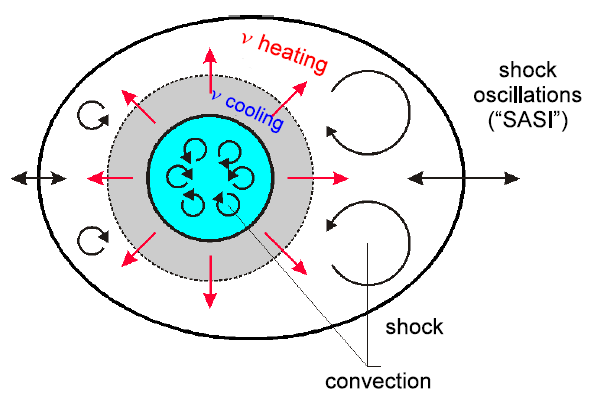
\includegraphics[width=4in]{figures/neutrino_model_diagram.png}
    \caption{Diagram of the neutrino model. Grey coloring represents the accretion layer around the PNS (cyan). Neutrino heating drives convective overturn in the gain region behind the shock front. Picture reproduced from~\cite{muller2016core}.}
    \label{fig:neutrino_model}
\end{figure*}

The GW signals from neutrino model explosions typically contain most of their power between 100\,-1100\,Hz and last between $\sim$\,0.5\,-\,2\,s. Multiple predictable features are present in a typical neutrino model waveform, such as prompt convection after core bounce, low frequency SASI emission below $\sim260$\,Hz, and a g-mode signal that rises in frequency and amplitude~\cite{andresen:16, kuroda:16, 2017arXiv170107325Y}. G-modes use buoyancy as a restoring force and represent oscillations in the PNS. These modes can be instigated from the inner core or at the surface via accreting mass that impinges upon the PNS~\cite{andresen:16, kuroda:16, 2017arXiv170107325Y}. For a source 10\,kpc away, the neutrino model produces a maximum strain of order $\sim10^{-22}$. The total energy emitted in GWs from a neutrino model CCSN is of order $\sim10^{-11}$\,-\,$10^{-9}M_\odot$~\cite{thesis_jade, thesis_josh}. Despite the fact that most simulations still fail to explode, the neutrino model represents the most likely shock revival mechanism in CCSNe.

\subsection{The Magnetorotational Model}

The magnetorotational model was first proposed in the early 1970s~\cite{bisnovatyi1970explosion, ostriker1971pulsars, meier1976magnetohydrodynamic, bisnovatyi1976magnetohydrodynamic} and relies on a rapidly rotating progenitor and highly magnetized PNS. Enormous rotational energy and magnetohydrodynamical (MHD) physics lead to matter being violently expelled away from the star. The initial toroidal component of the magnetic fields for progenitors is predicted to be of order $\sim10^{9}$\,G~\cite{heger2005presupernova}, but simulations have shown that a magnetic field of order $\sim10^{15}$\,G is necessary to power a magnetorotational CCSN~\cite{burrows2007simulations}. This means that magnetic amplification is typically required. The non-radial magnetic field component is expected to increase by a factor greater than $\sim1000$ as mass accretes onto the PNS~\cite{janka}, but further amplification can come from a winding of the poloidal field into the toroidal field. This stretching of the field lines essentially taps into the enormous reservoir of rotational energy. Magnetic fields can also grow exponentially due to the magnetorotational instability (MRI~\cite{balbus1998instability, akiyama2003magnetorotational}) which can grow out of the core~\cite{obergaulinger2009semi}. These amplification processes all require differential rotation, which is a natural result of infall. 

\begin{figure*}[b!]
    \centering
    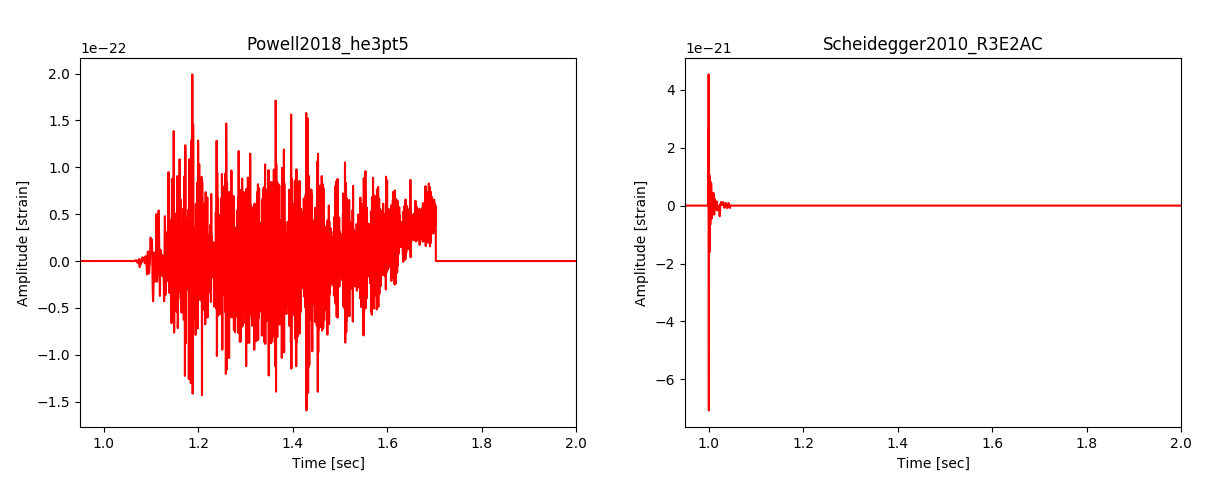
\includegraphics[width=\textwidth]{figures/Two_waveforms_6.png}
    \caption{Example GW signals for the neutrino model (left) and magnetorotational model (right). Core bounce is at t = 1\,s. Neutrino model waveforms typically exhibit sustained, stochastic GW emission, whereas magnetorotational waveforms release their GW energy in a strong burst at core bounce.}
    \label{fig:two_waveforms}
\end{figure*}

It's possible that collimated bipolar jets commonly propel matter along the rotation axis in such CCSN events~\cite{burrows2007simulations, akiyama2003magnetorotational, wheeler2002asymmetric}. The magnetorotational model requires the pre-collapse core to have a spin period less than $\sim2$\,-\,5\,s~\cite{burrows2007simulations, thompson2005viscosity}, which will then experience a frequency ``spin-up" factor of $\sim1000$ after collapse~\cite{ott2006spin}. Stellar evolution models predict that CCSN progenitors will typically have pre-collapse spin periods significantly longer than that~\cite{heger2005presupernova}, potentially even greater than $\sim100$\,s~\cite{janka}. This means that the magnetorotational model requires alternative stellar evolution theories or unusual progenitor birth conditions. It's expected that rapid rotation is present in less than 10\% of progenitor stars~\cite{heger2005presupernova, langer2012presupernova}.

The GW signal from a magnetorotational CCSN is dominated by broadband emission right at core bounce. This spike can be seen in Figure~\ref{fig:two_waveforms}. Rapid rotation causes the core to be deformed by momentum. When the core collapses, the derivatives of the quadrupole moment change significantly and a burst of GWs is emitted. These GWs are heavily dependent on viewing angle and for most magnetorotational simulations the GW energy is primarily found in one component (plus). Other GW features that are commonly found in neutrino model waveforms, such as SASI and g-modes, are less pronounced in rapidly rotating models. This is because rapid rotation can damp convection and because most magnetorotational simulations are short-lived. For a source at 10\,kpc, the magnetorotational model will have a peak strain of $\sim10^{-21}$\,-\,$10^{-20}$ and emit energy in GWs of order $\sim10^{-10}$\,-\,$10^{-8}M_\odot$~\cite{thesis_jade}. The magnetorotational model typically emits more power in GWs than the neutrino model, despite the fact that GWs are only emitted for tens of milliseconds. Most of the power in GWs is between 500\,-\,800\,Hz, but some of the most rapidly rotating models are dominated by centrifugal effects and result in GW emission primarily below $\sim200$\,Hz~\cite{ott2009recent, dimmelmeier2008gravitational}.

\subsection{Other Models}

Other shock revival mechanisms have been proposed, such as the acoustic model~\cite{burrows2007features}. In this model, SASI induces g-modes in the PNS surface. These surface vibrations send large sound waves into the stellar medium. As these waves move down the density gradient away from the PNS they can steepen into secondary shocks that help heat the postshock region and drive the explosion~\cite{janka}. However, 3D simulations have been unable to prove the validity of this mechanism~\cite{marek2009delayed} and a serious counterargument has been proposed against this model~\cite{weinberg2008non}.

Another proposed model is the phase-transition mechanism~\cite{sagert2009signals, fischer2011core}. This model relies on a first-order hadron-to-quark matter phase transition within the core after bounce. As the temperature and pressure rise, the inner core can undergo a transition to pure quark matter. This causes the nuclear EoS to stiffen again, which leads to a second rebounding shock wave that quickly catches up to the first~\cite{sagert2009signals, fischer2011core}. The two core bounces are enough to power the explosion. While this is an interesting theory, the fine-tuning of the quantum chromodynamics (QCD) phase transition is problematic and the hybrid nuclear EoSs that have been used are not compatible with real life stellar observations~\cite{janka}. None of the CCSN GW simulations used in this thesis model the acoustic or phrase-transition mechanisms.

\section{Asymmetries in CCSNe}

Asymmetries are required for the emission of GWs and numerous observations have suggested their presence in CCSNe. The most convincing data comes from measurements of pulsar kicks from recently exploded supernovae, which show average remnant neutron star space velocities of about 400\,km/s and maximum velocities above 1000\,km/s~\cite{hobbs2005statistical}. These values are considered too high to be explained by the breakup of binary systems, which means a natal kick is required~\cite{lai2001pulsar}. Anisotropic emission of gas can only account for neutron star velocities of about 200\,km/s via momentum conservation~\cite{janka1994neutron}. Another way to instigate asymmetrical evolution is to initiate a CCSN simulation with an asymmetrical progenitor~\cite{burrows1996pulsar, arnett2011toward}. Asymmetrical ram pressure can then result in a preferred direction for the explosion to propagate. While this can be effective in simulations, these progenitors are not compatible with our current understanding of stellar evolution models.

Anisotropic neutrino emission is another potential source of asymmetry. An asymmetry of 1\% in the total neutrino energy loss would be sufficient to kick the neutron star to more than 300\,km/s~\cite{janka}. However, the calculated pulsar kicks from anisotropic neutrino emission due to postbounce accetion~\cite{scheck2006multidimensional, wongwathanarat2010hydrodynamical} and convection~\cite{blaschke2001physics} have been estimated to be only $\sim10$\,km/s. It is not fully understood how sufficiently anisotropic neutrino emission would be produced.

Scheck et al.~\cite{scheck2006multidimensional, scheck2004pulsar} proposed the most promising explanation for remnant neutron star velocities. They realized that anisotropically emitted gas would result in long duration anisotropic gravitational forces on the neutron star. They calculated typical final kick velocities in the hundreds of km/s, with extremely anisotropic emission resulting in kick velocities greater than $\sim1000$\,km/s~\cite{scheck2006multidimensional}. This model has been confirmed in 3D~\cite{wongwathanarat2010hydrodynamical}, but the full explanation of where and how this asymmetrical emission originates is not fully understood. The rapid spins of remnant neutron stars is a further complication that is hard to explain without progenitor rotation~\cite{heger2005presupernova, ott2006spin}. Convection, along with hydrodynamical instabilities such as SASI, can establish angular momentum separation between the PNS and ejecta that may lead to significant remnant rotation despite a non-rotating progenitor~\cite{blondin2007pulsar, fernandez2010spiral}. The turbulent motion from SASI and convection is also expected to disrupt the well-stratified onion-shell structure of the progenitor~\cite{kifonidis2006non}, which may contribute to anisotropic emission of gas or neutrinos.

\section{CCSN Rates and Detection Prospects}
\label{sec:rates}

LIGO's initial CCSN search paper~\cite{abbott2016first} estimated the detection efficiency as a function of distance for various models. Pre-dating the advanced detector era, their results were sobering. Neutrino model waveforms had a 50\% detection efficiency at about .2\,kpc, while magnetorotational waveforms had a 50\% efficiency at approximately 1\,kpc~\cite{abbott2016first}. LIGO has recently published their second CCSN search paper based on advanced detector data from O1 and O2. Contemporary detectors are able to detect neutrino model waveforms with a 50\% efficiency at about 2\,kpc, while magnetorotational waveforms had the same efficiency at approximately 20\,kpc.

Estimates of the CCSN rate usually put it between 1\,-\,2 per galaxy per century~\cite{1991ARA&A..29..363V, 1993A&A...273..383C, Alexeyev2002}. If we assume that most CCSN resemble the neutrino model, which is currently the best assumption, then we would need a very nearby galactic CCSN to have any hope of a detection with current detectors. Considering the expected CCSN rate, this is unlikely. Future GW detectors, such as LIGO Voyager~\cite{2015PhRvD..91h2001D, voyagerupgrade}, the Einstein Telescope~\cite{0264-9381-27-19-194002, ET:design}, or LIGO Cosmic Explorer~\cite{2017CQGra..34d4001A, whitepaper2018}, will have drastically reduced noise floors and greatly extended ranges. By the time 3rd generation detectors are operational neutrino model waveforms should be consistently detectable between 100\,-\,150\,kpc, while magnetorotational waveforms should be detectable beyond 600\,-\,700\,kpc~\cite{roma2019astrophysics}. There are a dozen or so known galaxies, mostly satellite or dwarf, within the range of 60 kpc, 28 within the range of 150\,kpc, and 55 within the range of 790\,kpc (the distance to Andromeda)~\cite{karachentsev2004catalog, belokurov2007cats}. As improved detectors come online over the next few decades, a GW detection from a CCSN will become increasingly plausible.

\section{Waveform Simulations}

This section will summarize CCSN gravitational waveforms and models from different simulation groups. 1D and 2D CCSN simulations have been performed for decades and there are many publications exploring the GW emission \cite{muller2004toward, ott2006new, kotake2007gravitational, marek2009equation, yakunin2010gravitational, dimmelmeier2008gravitational}. Simulating a CCSN is famously difficult as multiple forces must be incorporated in an energetically dense and relativistic region of spacetime. Most simulations fail to explode, leading to uncertainty about the shock revival mechanism as described in section \ref{sec:mechanisms}\,. In recent years, advancements have allowed for full 3D simulations that incorporate neutrino physics and general relativity. These simulations have shown modified GW emission from their 2D counterparts but still typically fail to explode. Only 3D CCSN simulations will be presented and used in this thesis. An overview of the CCSN process, including simulation issues and uncertainties, can be found in~\cite{muller2016core}. Figure \ref{fig:example_waveforms} shows example waveforms from each simulation group.

\subsection{Scheidegger}

Scheidegger et al. \cite{scheidegger:10b, scheidegger2010gravitational} produce 25 3D magnetorotational waveforms from a $15M_\odot$ progenitor with varying levels of rotation. The 15 most rapidly rotating models are used in this thesis. The magnetohydrodynamics code of Pen et al.~\cite{pen2003free} and Liebend\"orfer et al.~\cite{liebendorfer2006efficient} is utilized along with two nuclear EoSs, one from Lattimer \& Swesty~\cite{lattimer1991generalized} and one from Shen et al.~\cite{shen1998relativistic}. For the neutrino physics, a parameterized deleptonization scheme is used that incorporates sophisticated computational techniques~\cite{liebendorfer2005simple} but is only valid for a few milliseconds after core bounce.

The GW emission is dominated by a broadband spike at core bounce due to the deformation of a rapidly rotating star and its changing quadrupole moment. Emission continues after bounce but is somewhat reduced due to damped convection in the case of rapid rotation. These simulations are also stopped no later than 130\,ms after core bounce. For these reasons, SASI and g-mode emission is less prominent and won't be considered for magnetorotational waveforms.

\begin{figure*}[p]
    \centering
    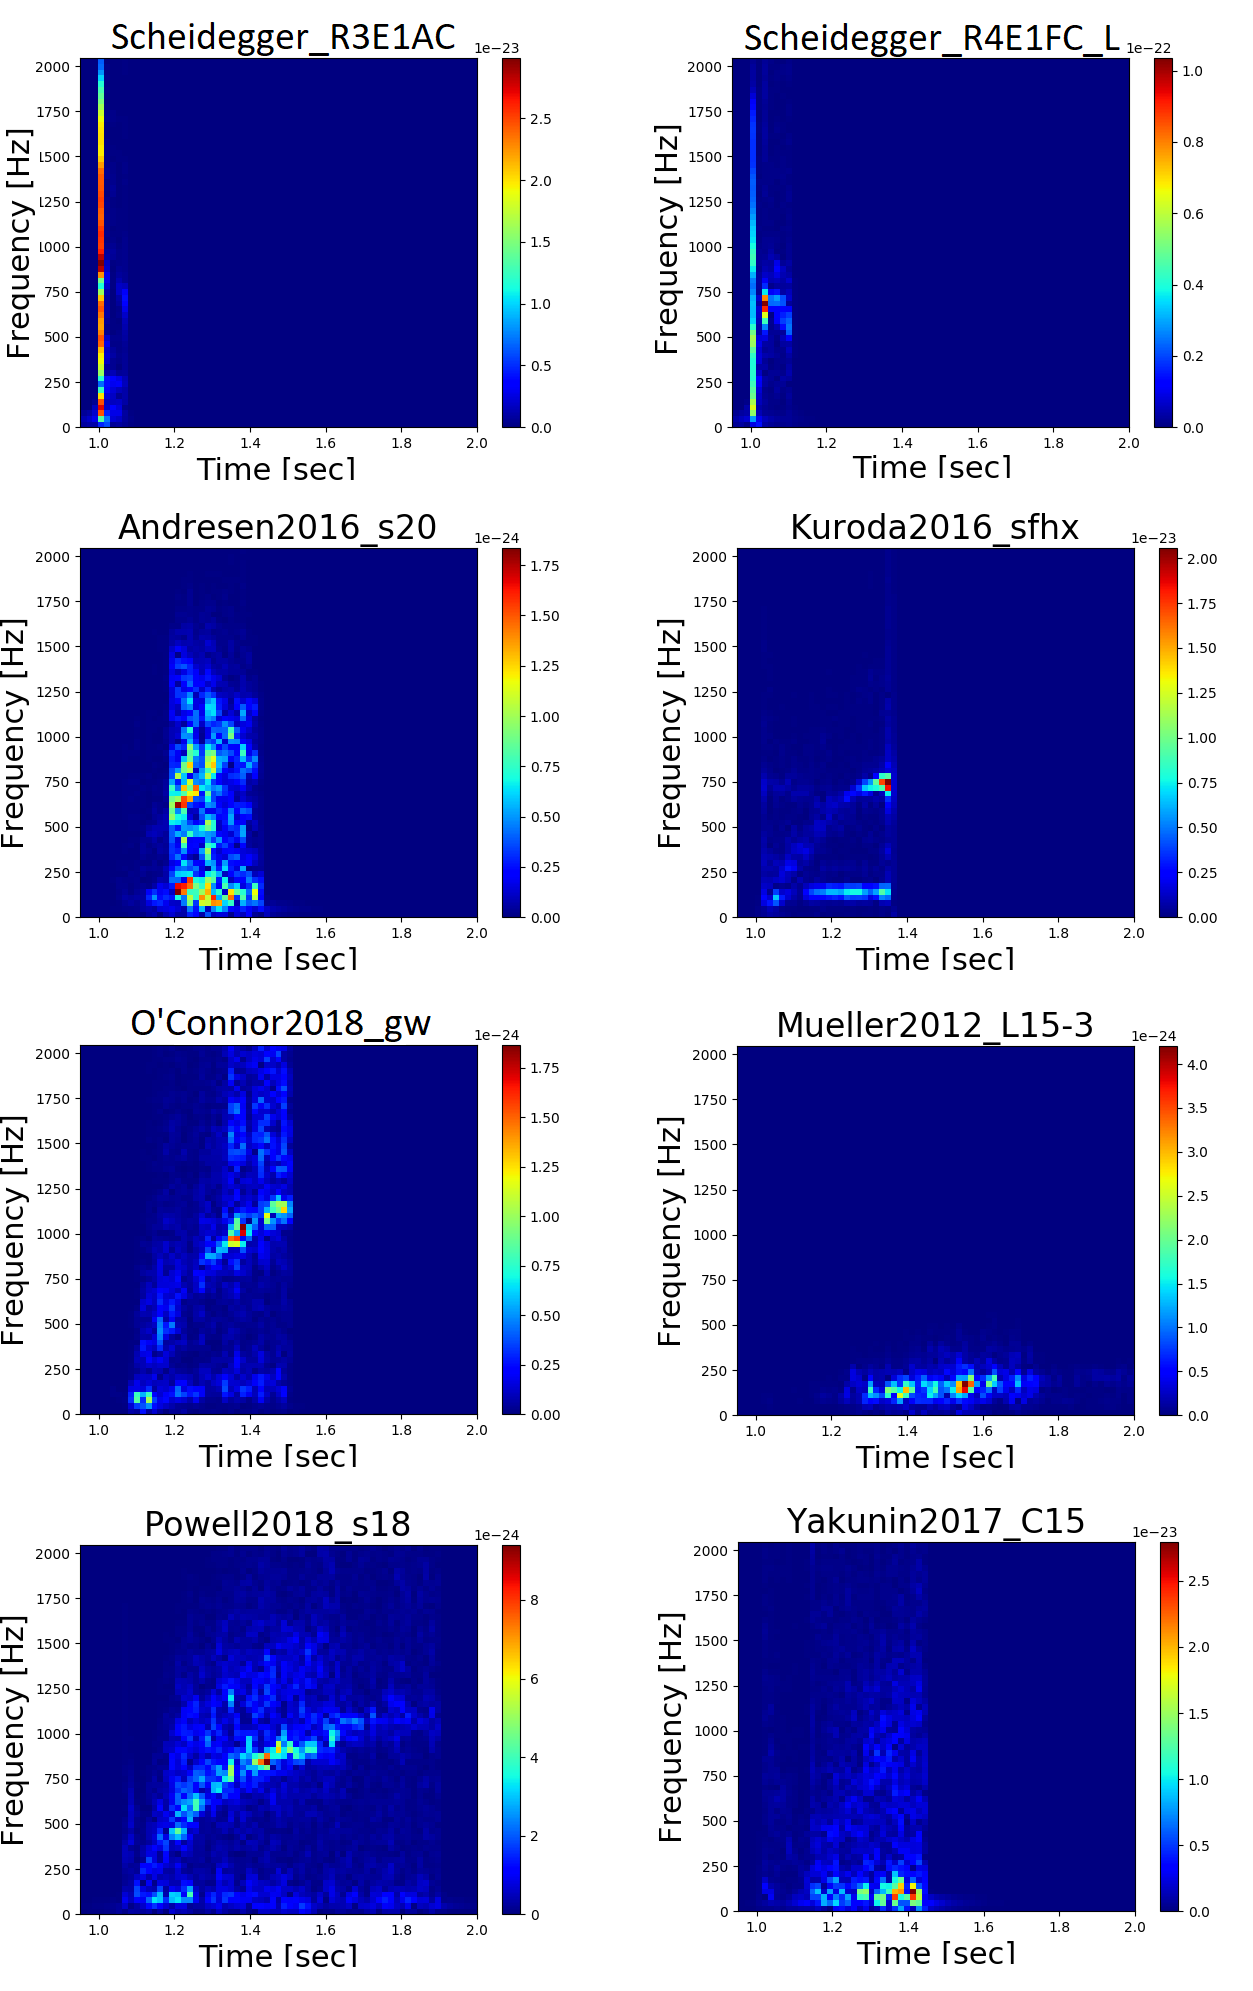
\includegraphics[height=7.9in]{figures/waveform_examples.png}
    \caption{Example waveforms from each simulation group. Two Scheidegger examples are shown as they are the only magnetorotational models used in this thesis. Core bounce is at t = 1\,s in all plots.}
    \label{fig:example_waveforms}
\end{figure*}

\subsection{Andresen}

Andresen et al.~\cite{andresen:16, andresen2018gravitational} have published four simulated neutrino-driven waveforms for non-rotating progenitors. These were 3D multi-group hydrodynamic simulations of progenitors with $11.2M_\odot$ (model s11), $20M_\odot$ (models s20 and s20s), and $27M_\odot$ (model s27). These simulations were created with the PROMETHEUS-VERTEX code~\cite{rampp2002radiation, fryxell1991instabilities}, which combines the Newtonian hydrodynamics module PROMETHEUS~\cite{muller1991instability, fryxell1991instabilities} with the neutrino-transport module VERTEX~\cite{rampp2002radiation}. The effects of general relativity are approximated with a pseudo-relativistic effective potential (case A in~\cite{marek2006exploring}). All four simulations used the Lattimer \& Swesty nuclear equation of state (EoS)~\cite{lattimer1991generalized}.% with a bulk incompressibility modulus for nuclear matter of $K = 220\,$MeV~\cite{lattimer1991generalized}.

Low frequency SASI-related GW emission is significant for all waveforms except model s11. That particular model's shock radius was too large to facilitate the growth of SASI. Instead, its emission is dominated by convection and related high frequency g-modes in the surface of the PNS. This high frequency g-mode emission was present in all four models, but is considered unreliable above 1000\,Hz due to aliasing problems related to the low sampling rate. The duration of the signals varies from 350 ms to 600 ms after core bounce. Model s20s includes modified strange quark interactions for neutral-current neutrino-nucleon scattering~\cite{melson2015neutrino} and was the only model to successfully revive the shock and explode as a CCSN.

\subsection{Kuroda}

Kuroda et al. carry out fully relativistic 3D simulations of a $15M_\odot$ ZAMS progenitor star using three different EoSs~\cite{kuroda:16}. Two of those models, sfhx and tm1, are used in this thesis. They differ from each other in their EoS and treatment of nuclear interactions, with tm1 following~\cite{hempel2010statistical} and sfhx following~\cite{steiner2013core}. Model sfhx is the ``softest" EoS and has the smallest radius. Both models use a $15M_\odot$ star from Woosley \& Weaver~\cite{woosley1995evolution} as the progenitor.

A rising g-mode signal is visible in both Kuroda waveforms. This emission is sourced by oscillations of the PNS surface and grows in frequency over time due to mass accretion. Kuroda et al. find that the growth of SASI is dependent upon the stiffness of the nuclear EoS, with the softest EoS facilitating SASI. Model sfhx therefore has a strong low frequency signal due to sloshing and spiral motions of the SASI, while tm1 does not. Neutrino-driven convection eventually dominates in both models. The simulations were stopped 340\,ms after core bounce.

\subsection{O'Connor/Couch}

This thesis uses 5 neutrino model waveforms from Evan O'Connor and Sean Couch~\cite{o2018exploring}. These simulations use the FLASH hydrodynamics framework that has been outfitted for CCSNe~\cite{couch2013impact, couch2014high}. Multidimensional energy-dependent neutrino-radiation transport based on the moment formalism is included along with effective general relativistic gravity~\cite{o2018two}. All models used a $20M_\odot$ solar metallicity progenitor from Farmer et al.~\cite{farmer2016variations} and the SFHo nuclear EoS from Steiner et al.~\cite{steiner2013core}.

High frequency g-modes were present in every waveform, while late-forming SASI was present in all but one. None of the simulations successfully exploded before being terminated 500\,ms after core bounce. Peak GW emission occurs anywhere from 600\,-\,1250\,Hz in different models. Model v\_LR\_gw differs from other simulations in that it has significant low frequency emission without the formation of SASI. GW emission in this case is reported to be due to turbulent kinetic energy in the gain region.

\subsection{M\"uller}

Three non-rotating neutrino model waveforms are featured from M\"uller et al.~\cite{mueller:e12}. Two of these simulations, models L15 and W15, used $15M_\odot$ progenitors while the other, model N20, used a $20M_\odot$ progenitor. A version of the multi-fluid hydrodynamics code PREMETHEUS~\cite{muller1991instability, fryxell1991instabilities} is once again utilized. Self-gravity is accounted for by solving Poisson's equation in integral form as an expansion into spherical harmonics. The potential's monopole term is corrected for general relativistic effects as described in~\cite{scheck2006multidimensional, arcones2007nucleosynthesis}. ``Ray-by-ray" neutrino transport and neutrino-matter interactions are approximated as in~\cite{scheck2006multidimensional}, while the tabulated EoS from Janka \& M\"uller~\cite{janka1996neutrino} is used to describe the stellar fluid.

Low frequency GW emission was extended as these simulations artificially prescribed the contraction of the PNS. The longest waveform extends to 1.3\,s after core bounce, but the strongest emission happens in the first .7\,s after bounce. Both SASI and g-modes are present in the signals, but the g-modes are slow to develop and rarely approach 300\,Hz. More recent simulations have shown g-mode emission at significantly higher frequencies~\cite{andresen:16, kuroda:16}.

\subsection{Powell}

Powell et .al~\cite{2018arXiv181205738P} carry out two neutrino-driven simulations with the neutrino hydrodynamics code CoCoNut-FMT. A general relativistic finite-volume based solver is used for the equations of hydrodynamics~\cite{muller2010new,dimmelmeier2002relativistic}. As opposed to previous simulations with CoCoNut-FMT, these extended down to the innermost $\sim$ 10\,km to include the PNS convection zone and impose spherical symmetry inside this radius. The neutrino transport is handled using the fast multigroup transport method of M\"uller \& Janka~\cite{muller2015non} with updates to the neutrino rates to be compatible with current experimental constraints and theoretical expectations \cite{hobbs2016role}. The nuclear EoS from Lattimer \& Swesty~\cite{lattimer1991generalized} is used for high density regions. Two models were produced with different progenitors. The first, model he3.5, is an ultra-stripped star in a binary that was evolved from a helium star with an initial mass of $3.5M_\odot$. This is the first GW signal to be produced from an ultra-stripped simulation. The second model used a ZAMS mass of $18M_\odot$ and is referred to as s18.

Both simulations exploded successfully and modelled the emission up to 0.8\,s after core bounce, well into the explosion phase. GW emission is dominated by a surface g-mode induced signal that rises in frequency and peaks between 800\,-\,1000\,Hz. Neither model had SASI activity or significant GW emission at low frequencies.

\subsection{Yakunin}

Yakunin et al.~\cite{yakunin2010gravitational, 2015PhRvD..92h4040Y, 2017arXiv170107325Y} produce one general relativistic, multi-physics, 3D simulation of a $15M_\odot$ progenitor with state of the art weak interactions. The progenitor of Woosley \& Heger~\cite{woosley2007nucleosynthesis} was used and the simulation was carried out with the CHIMERA code, which includes multigroup flux-limited diffusion neutrino transport, and an effective gravitational potential with general relativistic monopole and commensurate corrections to the neutrino transport~\cite{bruenn2016development}. The Lattimer \& Swesty EoS~\cite{lattimer1991generalized} was used for highest density regions and the Cooperstein EoS~\cite{cooperstein1985equation} was used for the lower density regions.

There is a significant quiescent phase after core bounce with little GW emission for 120\,ms. After that point, SASI activity becomes significant and GW emission is instigated. Peak GW emission occurs at about 1000\,Hz due to oscillations in the PSN surface. The simulation is cut off 450\,ms after core bounce. The GW amplitudes in this waveform are significantly larger than those from other simulation groups.


\chapter{Supernova Model Evidence Extractor}
\label{chp:SMEE}

The Supernova Model Evidence Extractor (SMEE) is a parameter estimation tool for GWs from CCSNe. It performs Bayesian model selection to make classification statements about an observed waveform. Due to the inherently random nature of CCSN waveforms, we decompose a catalog of related waveforms into principal components (PCs) that contain the most prominent features of a catalog. These PCs are then used to produce waveform reconstructions and perform model selection. Our waveforms and PCs are in the form of real-valued ASD spectrograms and depend only on the time and frequency of GW emission in order to be as robust as possible against the stochastic nature of CCSN signals. This chapter will explain the methodology and inner workings behind SMEE's algorithm.

\section{Bayesian Inference}

Bayesian Inference is a powerful analysis technique that has become common in astrophysics and other fields. It allows for the comparison of hypotheses while continuously accounting for new data. Bayes theorem can be thought of as relating the probability that a hypothesis is true to the more useful probability that our measured data would be observed given that the hypothesis is true~\cite{thesis_josh}. Explicitly, 
\begin{equation}
\label{equ:Bayes}
    p(H|D) = \frac{p(H)p(D|H)}{p(D)}
\end{equation}
where $p(H|D)$ is the posterior probability, $p(H)$ is the prior probability, $p(D|H)$ is the model evidence, and $p(D)$ is the probability of obtaining the data $D$ independently of the hypothesis, also called a marginal probability. The posterior probability represents what we know about a hypotheses after considering all of the data and previously known information. It is commonly the final desired result of probability calculations. The prior probability represents what is known about the hypothesis before considering the data. For many situations involving supernovae it is common to make as few assumptions as possible, meaning that some parameter prior distributions are frequently flat or constant across a given parameter space. The model evidence, $p(D|H)$, tells us how well the observed data agrees with what we would expect given our model to be true. This is the most important term for model selection.

When two hypotheses, or models, need to be compared to each other, it useful to take a ratio of their posterior probabilities. This is known as an odds ratio~\cite{thesis_josh, thesis_jade},
\begin{equation}
\label{equ:Odds}
    O_{ij} = \frac{p(M_{i}|D)}{p(M_{j}|D)} = \frac{p(M_{i})p(D|M_{i})}{p(M_{j})p(D|M_{j})} = \frac{p(M_{i})}{p(M_{j})}B_{ij}
\end{equation}
where $B_{ij}$ is a Bayes factor defined as the ratio of model evidences,
\begin{equation}
    B_{ij} = \frac{p(D|M_{i})}{p(D|M_{j})}
\end{equation}
It's worth noting that when we plug equation \ref{equ:Bayes} into our odds ratio the denominator factors out as it is the same for each model. If neither model is preferred a priori, then $p(M_{i}) = p(M_{j})$ and the odds ratio simplifies to a Bayes factor. This Bayes factor is the primary output of a model selection algorithm such as SMEE. For a model defined by a set of parameters, the model evidence, $Z$, can be calculated by integrating the likelihood, $p(D|\theta,M)$, multiplied by the prior, $p(\theta|M)$, across all parameter values $\theta$,
\begin{equation}
\label{equ:evidence_def}
    Z = p(D|M) = \int_{\theta} p(\theta|M)p(D|\theta,M)d\theta
\end{equation}
This integral is commonly difficult or impossible to solve analytically, leading to the use of numerical techniques such as nested sampling~\cite{thesis_josh, thesis_jade, logue:12, powell:16b, 2017PhRvD..96l3013P}.

\section{Power Spectral Density and Likelihood}

Our statistics depend on the power of GW emission in a frequency bin. Specifically, we calculate the power spectral density for each tile in our spectrograms. The two-sided PSD is defined~\cite{miller2012probability}, 
\begin{equation}
\label{equ:PSD_def}
    S_{xx}(f) = \lim_{T \to \infty} \left\langle |\tilde{d}(f)|^{2} \right\rangle
\end{equation}
where the brackets indicate an expectation value and $\tilde{d}(f)$ is a Fourier transform of detector data defined as,
\begin{equation}
    \tilde{d}(f) = \frac{1}{\sqrt{T}} \int_{0}^{T} d(t)e^{-2\pi it}dt
\end{equation}
Technically, SMEE approximates a PSD by calculating a periodogram at each time in the spectrogram. Essentially this means that there is no infinite limit or averaging in equation \ref{equ:PSD_def}\,. The accuracy of our PSDs with respect to random detector noise could be improved by averaging over more time, but this also lowers signal amplitudes and offered no performance improvement in our testing. Rewriting equation \ref{equ:PSD_def} gives,
\begin{equation}
\label{equ:PSD_approx}
    S_{xx}(f) \approx |\tilde{d}(f)|^{2} = \mathbb{R}[\tilde{d}(f)]^{2} + \mathbb{I}[\tilde{d}(f)]^{2}
\end{equation}
where $\mathbb{R}$ and $\mathbb{I}$ represent the real and imaginary parts of the Fourier transform respectively. Equation \ref{equ:PSD_approx} shows explicitly that our PSD approximation is a sum of two squared numbers. For Gaussian noise it can be shown that these will both be Gaussian variables. Detector data can be written as the linear sum of Gaussian noise and a GW signal~\cite{veitch:15},
\begin{equation}
\label{equ:d_def}
    \tilde{d}(f) = \tilde{n}(f) + \tilde{h}(f)
\end{equation}
For Gaussian noise,
\begin{equation}
\label{equ:gaus_noise}
    \left\langle \tilde{n}(f) \right\rangle = 0 \quad\text{and}\quad \left\langle |\tilde{n}(f)|^{2} \right\rangle = \sigma_{f}^{2} = \frac{S(f)}{2}
\end{equation}
where $S(f)$ is the one-sided noise spectral density. The leftmost equality tells us that the expectation value of the detector data Fourier transform is equal to the Fourier transform of the signal.
\begin{equation}
\label{equ:d_mean}
    \left\langle \tilde{d}(f) \right\rangle = \tilde{h}(f) %\quad\text{and}\quad \left\langle |\tilde{d}(f)|^{2} \right\rangle = |\tilde{h}(f)|^{2}
\end{equation}
Looking back at equation \ref{equ:PSD_approx}, the right-hand side is the sum of two squared Gaussian variables. Each variable has a mean determined by the signal (as seen in equation \ref{equ:d_mean}) and a variance determined by the detector noise (right-hand side of equation \ref{equ:gaus_noise}). If these were Gaussian variables with unit variance then this would resemble a noncentral chi-squared distribution with two degrees of freedom. In order to obtain unit variance, we must divide our variables by their current variance. The right side of equation \ref{equ:gaus_noise} tells us the variance for Gaussian noise. The variance of the real and imaginary parts will be half of the total variance,
\begin{equation}
    \left\langle |\tilde{n}(f)|^{2} \right\rangle = \left\langle \mathbb{R}[\tilde{n}(f)]^{2} \right\rangle + \left\langle \mathbb{I}[\tilde{n}(f)]^{2} \right\rangle
\end{equation}
This gives us,
\begin{equation}
    \sigma^{2} = \frac{S(f)}{4}
\end{equation}
Dividing through in equation \ref{equ:PSD_approx} gives,
\begin{equation}
    \frac{S_{xx}(f)}{\sigma^{2}} \approx \frac{\mathbb{R}[\tilde{d}(f)]^{2}}{\sigma^{2}} + \frac{\mathbb{I}[\tilde{d}(f)]^{2}}{\sigma^{2}}
\end{equation}
Plugging in $\sigma^{2}$ explicitly and replacing $S_{xx}$ with the one-sided PSD of detector data $S_{x}$ (where $S_{x} = 2S_{xx}$ for real data),
\begin{equation}
    \frac{2S_{x}(f)}{S(f)} \approx \frac{4\mathbb{R}[\tilde{d}(f)]^{2}}{S(f)} + \frac{4\mathbb{I}[\tilde{d}(f)]^{2}}{S(f)}
\end{equation}
This is the final result used by SMEE. Because we now have two squared Gaussian variables each with unit variance and nonzero mean, this can be represented by a noncentral chi-squared distribution.

We can do a quick sanity check by assuming momentarily that there is no signal present, $\tilde{h}(f) = 0$, and that our data consists entirely of Gaussian noise. With no signal present, our noncentral chi-squared distribution simplifies to a standard chi-squared distribution and,
\begin{equation}
    \left\langle S_{x}(f) \right\rangle = S(f)
\end{equation}
This leads immediately to an expectation value for our chi-squared variable,
\begin{equation}
    \left\langle \frac{2S_{x}(f)}{S(f)} \right\rangle = 2
\end{equation}
For Gaussian noise, our expectation value is equal to the number of degrees of freedom. This is as expected for a chi-squared variable~\cite{stats_shao}.

\section{Noncentral Chi-Squared Distribution}

If $(X_{1}, X_{2}, ... , X_{i}, ... , X_{k})$ are $k$ independent, normally distributed random variables with means $\mu_{i}$ and unit variances, then the sum of their squares, $x$, is a noncentral chi-squared variable~\cite{freedman2007statistics}.
\begin{equation}
    x = \sum_{i=1}^{k} X_{i}^{2}
\end{equation}
The noncentrality parameter, $\lambda$, is related to the means of each variable and is defined as,
\begin{equation}
    \lambda = \sum_{i=1}^{k} \mu_{i}^{2}
\end{equation}
The full probability density function depends only on $k$ and $\lambda$ and is defined,
\begin{equation}
\label{equ:chi_pdf}
    P(x|\lambda) = \frac{1}{2}e^{-(x + \lambda) / 2}\Big(\frac{x}{\lambda}\Big)^{k/4-1/2} I_{k/2-1}(\sqrt{x\lambda})
\end{equation}
where $I_{\alpha}$ refers to a modified Bessel function of the first kind. Plugging in $k = 2$, for two degrees of freedom, gives,
\begin{equation}
    P(x|\lambda) = \frac{1}{2}e^{-(x + \lambda) / 2}\,I_{0}(\sqrt{x\lambda})
\end{equation}
This is the likelihood for a single frequency bin. For a series of data points, such as the bins within a spectrogram, the total likelihood is the product of the likelihoods for each bin. SMEE actually calculates the $\log$ of the likelihood, which means the product becomes a sum, and for $N$ data points our signal likelihood becomes,
\begin{equation}
\label{equ:signal_like_N_def}
    \log \mathcal{L}_{S} = \sum_{n=1}^{N} \left( \log(1/2) - \frac{(x_{n} + \lambda_{n})}{2} + \log\Big(I_0(\sqrt{x_{n}\lambda_{n}})\Big) \right)
\end{equation}
A subscript $n$ has been added to $x$ and $\lambda$ to indicate that they differ for each bin.

The chi-squared variable that SMEE uses was defined in the previous section.
\begin{equation}
\label{equ:x_def}
    x = \frac{2S_{x}(f)}{S(f)} \approx \frac{2\,d_{n}^{2}}{S(f)}
\end{equation}
where $S_{x}(f)$ refers to a one-sided PSD of detector data and $S(f)$ is the one-sided noise spectral density. A new notation, $d_{n}\,$, is introduced above as the periodogram approximation of a one-sided ASD of detector data ($d_{n} = |\tilde{d}(f)|$). Its subscript $n$ indicates that it represents the power of a single bin within a spectrogram. Spectrograms consist of multiple PSDs at many different times, so $d_{n}^{2}\,$, the power in each bin, is a function of both frequency and time. Going forward, however, both $f$ and $t$ will be omitted from notation for the sake of brevity and presentation. The noncentrality parameter used in SMEE is,
\begin{equation}
\label{equ:lambda_def}
    \lambda = \frac{2\,h_{n}^{2}}{S(f)}
\end{equation}
where $h_{n}$ is a one-sided ASD of the signal. Once again, the subscript $n$ indicates that it represents the power of a single bin from within a spectrogram and is therefore a function of $f$ and $t$. One quick way to arrive at this result is to consider equation \ref{equ:d_mean}\,, which tells us that $\tilde{h}(f)$ is the mean of $\tilde{d}(f)\,$. Squaring that mean and dividing by the same variance we used to obtain our chi-squared variable ($\sigma^{2} = \frac{S(f)}{4}$) gives us equation \ref{equ:lambda_def}\,. We can also arrive at this result by considering the expectation value of our chi-squared variable. To do that, I will first take the absolute square and expectation value of equation \ref{equ:d_def}\,,
\begin{equation}
\label{equ:d2_def}
    \langle |\tilde{d}(f)|^{2} \rangle = \langle |\tilde{n}(f)|^{2} \rangle + \langle |\tilde{h}(f)|^{2} \rangle
\end{equation}
There are no cross terms because we assume that $\tilde{n}(f)$ and $\tilde{h}(f)$ are entirely independent of each other and $\langle \tilde{n}(f)\tilde{h}(f) \rangle = 0$\,. Rewriting this with our simpler one-sided ASD notation,
\begin{equation}
    \left\langle d_{n}^{2} \right\rangle = \left\langle n_{n}^{2} \right\rangle + \left\langle h_{n}^{2} \right\rangle
\end{equation}
The expectation value of our chi-squared variable is then,
\begin{equation}
    \begin{split}
    \left\langle \frac{2\,d_{n}^{2}}{S(f)} \right\rangle =& \left\langle \frac{2\,n_{n}^{2}}{S(f)} \right\rangle + \left\langle \frac{2\,h_{n}^{2}}{S(f)} \right\rangle \\
    =& \,\,2 + \frac{2\,h_{n}^{2}}{S(f)} \\
    =& \,\,k + \lambda
    \end{split}
\end{equation}
This is the correct result for a noncentral chi-squared variable and shows that $\lambda$ is properly defined~\cite{stats_shao, freedman2007statistics}.

We can now plug in $x$ and $\lambda$ from equations \ref{equ:x_def} and \ref{equ:lambda_def} into equation \ref{equ:signal_like_N_def} to get our final signal model likelihood,
\begin{equation}
\label{equ:signal_like_def}
    \log \mathcal{L}_{S} = N\log(1/2) + \sum_{n=1}^{N} \left( \frac{-(d_{n}^{2} + h_{n}^{2})}{S(f)} + \log\Big(I_0(\frac{2 d_{n} h_{n}}{S(f)})\Big) \right)
\end{equation}
where $d_{n}$ and $h_{n}$ represent one-sided ASDs of the detector data and signal respectively. This likelihood value represents how well our data fits our signal hypothesis. The noise likelihood represents how well our data fits the hypothesis of pure Gaussian noise. We can obtain the noise likelihood by setting $h_{n} = 0$ in equation \ref{equ:signal_like_def}\,. This is equivalent to using the standard chi-squared distribution with $k = 2\,$. In either case, for $N$ data points we obtain a final noise likelihood of,
\begin{equation}
\label{equ:noise_like_def}
    \log \mathcal{L}_{N} = N\log(1/2) - \sum_{n=1}^{N} \frac{d_{n}^{2}}{S(f)}
\end{equation}

Equation \ref{equ:signal_like_def} contains the signal model, $h_{n}\,$. This represents the CCSN signal hypothesized to be in the data. Our signal model has the units of an ASD and is constructed out of principal components. These principal components are created from simulated CCSN waveforms and will be discussed in the next section.

\section{Principal Component Analysis}
\label{sec:PCA}

PCA is performed on a catalog of waveforms to create a set of orthogonal basis vectors called Principal Components (PCs). The PCs contain the most important features of the waveforms in a catalog~\cite{logue:12, powell:16b, 2017PhRvD..96l3013P, heng:09}. For time domain signals, each input waveform is a simple vector. The signals used in SMEE are three second long zero-padded amplitude spectral density (ASD) spectrograms. Each successive ASD in a spectrogram is a vector, containing one power value for each frequency bin. We attach data from the second ASD to the back of the first, and so on, to create a single vector out of each spectrogram. We then create an $m \times n$ matrix $\textbf{D}$, where each row contains a waveform, $m$ is the number of waveforms in the catalog, and $n$ is the length of each waveform. The covariance matrix can be defined by,
\begin{equation}
    \label{equ:covariance}
    \textbf{C} = \frac{1}{m}\textbf{D}\textbf{D}^{T}
\end{equation}
In order to obtain a set of basis vectors that span the linear space of each column in $\textbf{D}$, we would like to find the normalized eigenvectors of $\textbf{C}$. This will allow us to uniquely represent each catalog waveform as a linear combination of these eigenvectors. While $m$ is typically on the order of $\sim$ 10, $n$ is usually orders of magnitude larger. This means the above factoring can be very computationally expensive. This problem can mitigated by instead calculating the eigenvectors, $\boldsymbol\Sigma$, of $\textbf{D}^{T}\textbf{D}$ such that,
\begin{equation}
    \textbf{D}^{T}\textbf{D}\boldsymbol\Sigma_{i} = u_{i}\boldsymbol\Sigma_{i}
\end{equation}
where $u_{i}$ is the corresponding eigenvalue for each eigenvector. If we pre-multiply each side by $\textbf{D}$, then,
\begin{equation}
    \textbf{D}\textbf{D}^{T}\textbf{D}\boldsymbol\Sigma_{i} = u_{i}\textbf{D}\boldsymbol\Sigma_{i}
\end{equation}
If we write equation \ref{equ:covariance} as $\textbf{C} = \textbf{D}\textbf{D}^{T}$ then $\textbf{U} = \textbf{D}\boldsymbol\Sigma_{i}$ are the eigenvectors of the covariance matrix. This means that the eigenvectors of the covariance matrix can be determined by calculating the eigenvectors of $\textbf{D}^{T}\textbf{D}$, which is a significantly smaller $m \times m$ matrix. This greatly reduces the computational cost~\cite{heng:09}.

After performing Singular Value Decomposition (SVD) on the matrix $\textbf{D}$, the data has been factored such that,
\begin{equation}
\label{equ:SVD}
    \textbf{D} = \textbf{U}\,\boldsymbol\Sigma\,\textbf{V}^{T}
\end{equation}
The columns of $\textbf{U}$ and $\textbf{V}$ contain the eigenvectors of $\textbf{D}\textbf{D}^{T}$ and $\textbf{D}^{T} \textbf{D}$, respectively \cite{heng:09}. $\boldsymbol\Sigma$ is a diagonal matrix with elements corresponding to the square roots of the eigenvalues. The PCs are the orthonormal eigenvectors in $\textbf{U}$ and are ranked by their eigenvalues in $\boldsymbol\Sigma$. The first few PCs contain the most important features of a catalog. Figure \ref{fig:PCs_example} shows example PCs for a three waveform catalog. After performing SVD our PCs are in the form of vectors, meaning that they must be chopped up and reassembled for use as spectrograms. This is simply the inverse of what was described above to turn them into vectors. If our ASDs contain $N$ frequency bins, then the first $N$ data points represent the first ASD in the spectrogram, the second $N$ data points represent the second ASD in the spectrogram, and so on.

\begin{figure*}[t]
    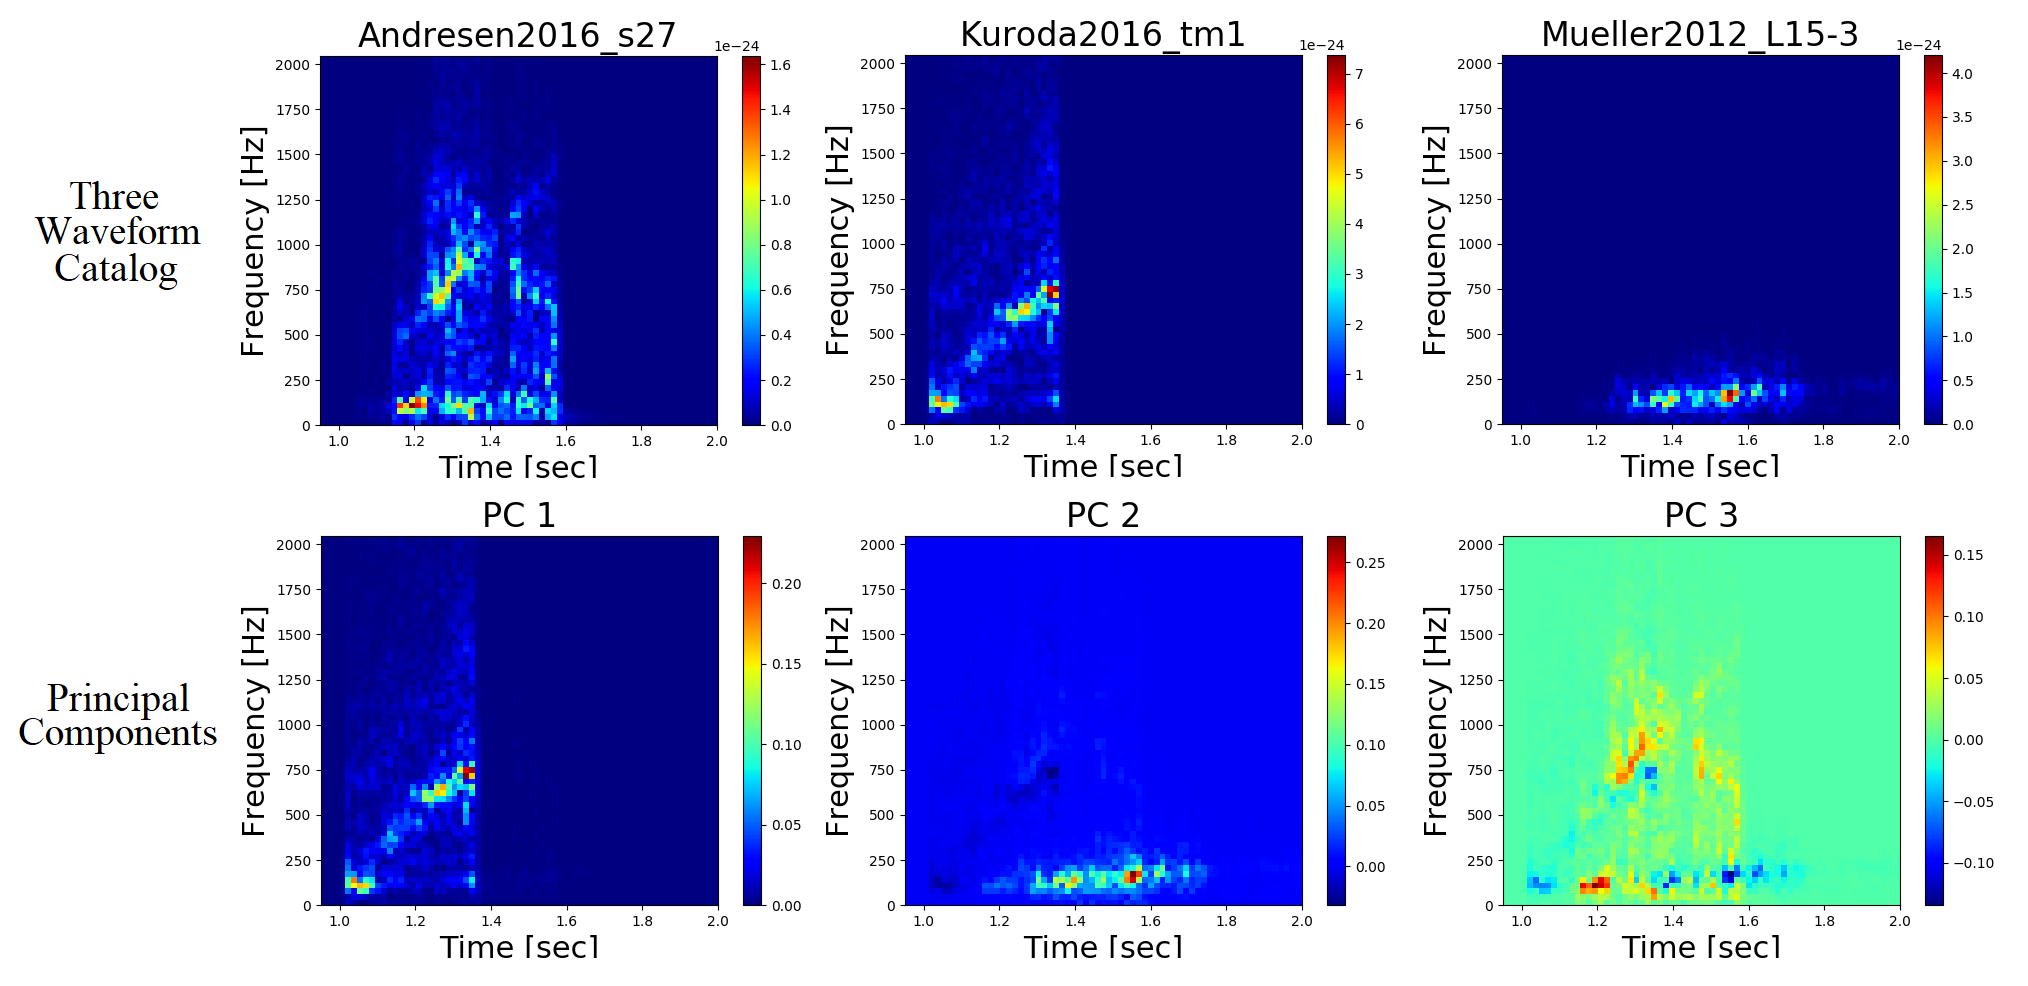
\includegraphics[width=\textwidth]{figures/PCs_example.png}
    \caption{PCs for an example catalog consisting of three neutrino model waveforms. The first PC looks very similar to the Kuroda2016\_tm1 waveform because that waveform has the largest $h_{rss}$ in this small catalog.}
    \label{fig:PCs_example}
\end{figure*}

As mentioned previously, the most important waveform features are contained in the first few PCs. In other words, PCA allows for a dimensional reduction in a data set. Catalog waveforms can usually be well-approximated with only a few PCs. The variance of the data set explained is a function of the number of PCs and is defined as~\cite{thesis_jade},
\begin{equation}
\label{equ:variance}
    v(k) = \frac{1}{\Lambda}\sum_{i=1}^{k} \Sigma_{i} \quad\text{where}\quad \Lambda = \sum_{i=1}^{n} \Sigma_{i}
\end{equation}
$\Sigma_{i}$ are the eigenvalues within $\boldsymbol\Sigma$ from equation \ref{equ:SVD}\,. Most of a catalog's variance can typically be explained by a subset of the total PCs.

A linear combination of PCs is used to construct our signal model, 
\begin{equation}
\label{equ:linear_sum}
    h_i \approx \left| \sum_{j=1}^{k} U_j \beta_j \right| \,,
\end{equation}
where $h_i$ is our reconstructed waveform (ASD spectrogram), $U_j$ is the $j$th PC, $\beta_j$ is the corresponding PC coefficient, and $k$ is the number of PCs being used. This reconstruction can then be used as a model for Bayesian model selection.

\section{Time-shifting the Signal Model} \label{sec:timeshift}

The signal model in equation \ref{equ:linear_sum} is essentially an ASD spectrogram of the signal. All of the waveforms used during the PCA are aligned in time via their times of core bounce. However, for a real CCSN signal in detector data the time of core bounce will likely not be known. Non-rotating and slowly-rotating CCSN simulations usually do not contain significant GW emission at core bounce and sometimes don't for another one or two hundred milliseconds after. Additionally, the time of arrival will be different in each detector for a multi-detector configuration. All of this means that SMEE must be able to move its signal model around in time in order to find the best reconstruction. SMEE's spectrograms contain only real data and therefore cannot be time-shifted through Fourier or similar techniques.

Our spectrograms contain 3 seconds of data and 191 individual PSDs. Each PSD is 0.03125 seconds long and has a 50\% overlap. That means the time step between subsequent PSDs is 0.015625 seconds. A spectrogram can be seen as a matrix where each column contains the PSD for a given time. The easiest way to time-shift our model is to simply shift all of our columns in one direction.  For example, shifting every column to the left by one would shift the signal model forward in time by 0.015625 seconds. The obvious concern with this method is what happens at the endpoints of the spectrogram. If we shift every column to the left by one, then the leftmost column, the first PSD, has nowhere to go. We get around this by shifting the columns in a circular fashion. If the columns are to be shifted to the left by one, then the first column would be moved to other end of the matrix to become the final column,
\begin{equation}
    \begin{bmatrix}
    1 & 4 & 7 \\
    2 & 5 & 8 \\
    3 & 6 & 9
    \end{bmatrix}
    \quad \Rightarrow \quad
    \begin{bmatrix}
    4 & 7 & 1 \\
    5 & 8 & 2 \\
    6 & 9 & 3
    \end{bmatrix}
\end{equation}
Similarly, if we were moving every column to the right by one then the rightmost column, the final column, would become the first column. We avoid issues at the endpoints by zero padding our waveforms on both sides,
\begin{equation}
    \begin{bmatrix}
    0 & 0 & 1 & 4 & 7 & 0 & 0 \\
    0 & 0 & 2 & 5 & 8 & 0 & 0 \\
    0 & 0 & 3 & 6 & 9 & 0 & 0
    \end{bmatrix}
    \quad \Rightarrow \quad
    \begin{bmatrix}
    0 & 1 & 4 & 7 & 0 & 0 & 0 \\
    0 & 2 & 5 & 8 & 0 & 0 & 0 \\
    0 & 3 & 6 & 9 & 0 & 0 & 0
    \end{bmatrix}
\end{equation}
All of our waveforms are aligned with their core bounces at t = 1 second. None of our waveforms are longer than 1.5 seconds, which means that every signal model reconstruction has at least 0.5 seconds of zero padding at the end. All of this together means that we can perform a circular time-shift up to 0.5 seconds in either direction without issues. For a real signal then, our estimated core bounce time must be within a half second of the actual core bounce time, which is very feasible. If we wanted to time-shift by more than 0.5 seconds we could simply increase the amount of zero padding. Lengthening our spectrograms from 3 to 4 seconds for example, would allow for 1 second time-shifts in either direction.

The main detriment to this method is the simple fact that our temporal resolution is limited to 0.015625 seconds. While this is not ideal, it is significantly shorter than typical CCSN waveforms and has not been a concern in testing.

\section{Priors}
\label{sec:priors}

The evidence in equation \ref{equ:evidence_def} for a given signal model depends on the following parameters: time (arrival at Earth geocenter), source position (right ascension, declination, and polarization angle), $h_{rss}$\,, and the PC coefficients in equation \ref{equ:linear_sum}\,. The number of PCs, and coefficients, is optional. After running SMEE to produce a Bayes factor, posterior distributions can be created for each parameter listed. In many situations the sky location will be known, in which case the right ascension and declination parameters will be constants obtained from astronomers.

SMEE's algorithm is initiated with an estimated arrival time chosen by the user. As discussed in the previous section, SMEE can time-shift its signal models 0.5 seconds in either direction. The prior distribution for time is then bounded 0.5 seconds before and after the estimated arrival time and has a flat (uniform) shape. When the sky position is unknown, right ascension is bounded between $[0, 2\pi]$ with a flat shape and declination is bounded between $[-\frac{\pi}{2}, \frac{\pi}{2}]$ with its shape uniform in cosine. The source polarization angle is always bounded between $[0, \pi]$ with a flat shape. The upper and lower bounds on $h_{rss}$ can be chosen by the user and the prior is uniform in volume. If the chosen lower bound is too small, then SMEE will always return $\log B_{S,N} \approx 0$ as the signal and noise models are statistically indistinguishable. The upper bound on $h_{rss}$ can be freely chosen as long as it is above the actual value.

The remaining parameters are the PC coefficients, all of which have flat, uniform priors. The upper and lower bounds for these can be determined in various ways, including simple experimentation. This process results in wider bounds for the first few PCs as they are typically more heavily used (have larger coefficients) in reconstructions. A more targeted approach is to calculate the dot product between each PC and each catalog waveform~\cite{thesis_josh, thesis_jade, heng:09}. Doing this will give the coefficients needed to reconstruct each catalog waveform out of the PCs. Once all of the these coefficients are known, the catalog minimum and maximum values can be found for each PC coefficient. The upper and lower prior bounds can then be set to these values plus or minus $\sim 10\%$\,. This gives bounds that are based upon the catalog waveforms but account for some simulation uncertainty.

\section{Nested Sampling}

In order to perform Bayesian model selection, SMEE must calculate the evidence integral in equation \ref{equ:evidence_def}\,. To do this, SMEE uses the LALInference Nested Sampling algorithm within LIGO's Algorithm Library (LAL)~\cite{thesis_jade, veitch:15}. Nested Sampling is a numerical technique that can solve evidence integrals and produce posterior distributions for the parameters of a model~\cite{thesis_josh}. The evidence can be written as,
\begin{equation}
\label{equ:evidence_algrebra}
    \begin{split}
    Z =& \int_{\theta} p(\theta|M)p(D|\theta,M)d\theta \\
    \approx& \sum_{i=1} p(D|\theta_{i},M)\omega_{i} \\
    \approx& \sum_{i=1} \mathcal{L}_{i}\omega_{i} \\
    \end{split}
\end{equation}
where $\omega_{i}$ is the weight, indicating the fraction of the prior distribution represented by the $i$th sample, and $\mathcal{L}_{i} = p(D|\theta_{i},M)$ is the likelihood. Initially, a set of data points is randomly chosen from the prior. Each of these ``live points" represent a possible waveform reconstruction and have likelihood values associated with them. The point with the lowest likelihood will have the largest prior mass, where prior mass, $X$, is defined,
\begin{equation}
\label{equ_prior_mass}
    X(\nu) = \int_{\mathcal{L}(\theta)>\nu} p(\theta|M)d\theta
\end{equation}
$\nu$ represents a likelihood value in the formula above. As $\nu$ increases, the prior mass, $X\,$, decreases. Each iteration of the nested sampling, the point with the lowest likelihood and largest prior mass will be replaced. The likelihood and prior mass values for that point are then used as limiting values for the replacement live point. This new live point is generated within those limiting values using Markov Chain Monte Carlo techniques~\cite{sivia1996data, thesis_jade}. This repeats with the live points iteratively converging upon the region of the prior with the highest likelihood. Figure \ref{fig:nested_sampling} illustrates this procedure. When a signal is present, the evidence integral will be dominated by this small region of the prior. This high likelihood region of the prior is concentrated in a fraction, $e^{H}$, of the parameter space. $H$ is referred to as the information in the data, and is defined,
\begin{equation}
    \begin{split}
    H =& \int \log \frac{dP}{dX}dP \\
    \approx& \sum p(\theta|D,M)\log\frac{p(\theta|D,M)}{dX} d\theta
    \end{split}
\end{equation}
\begin{figure*}[t!]
    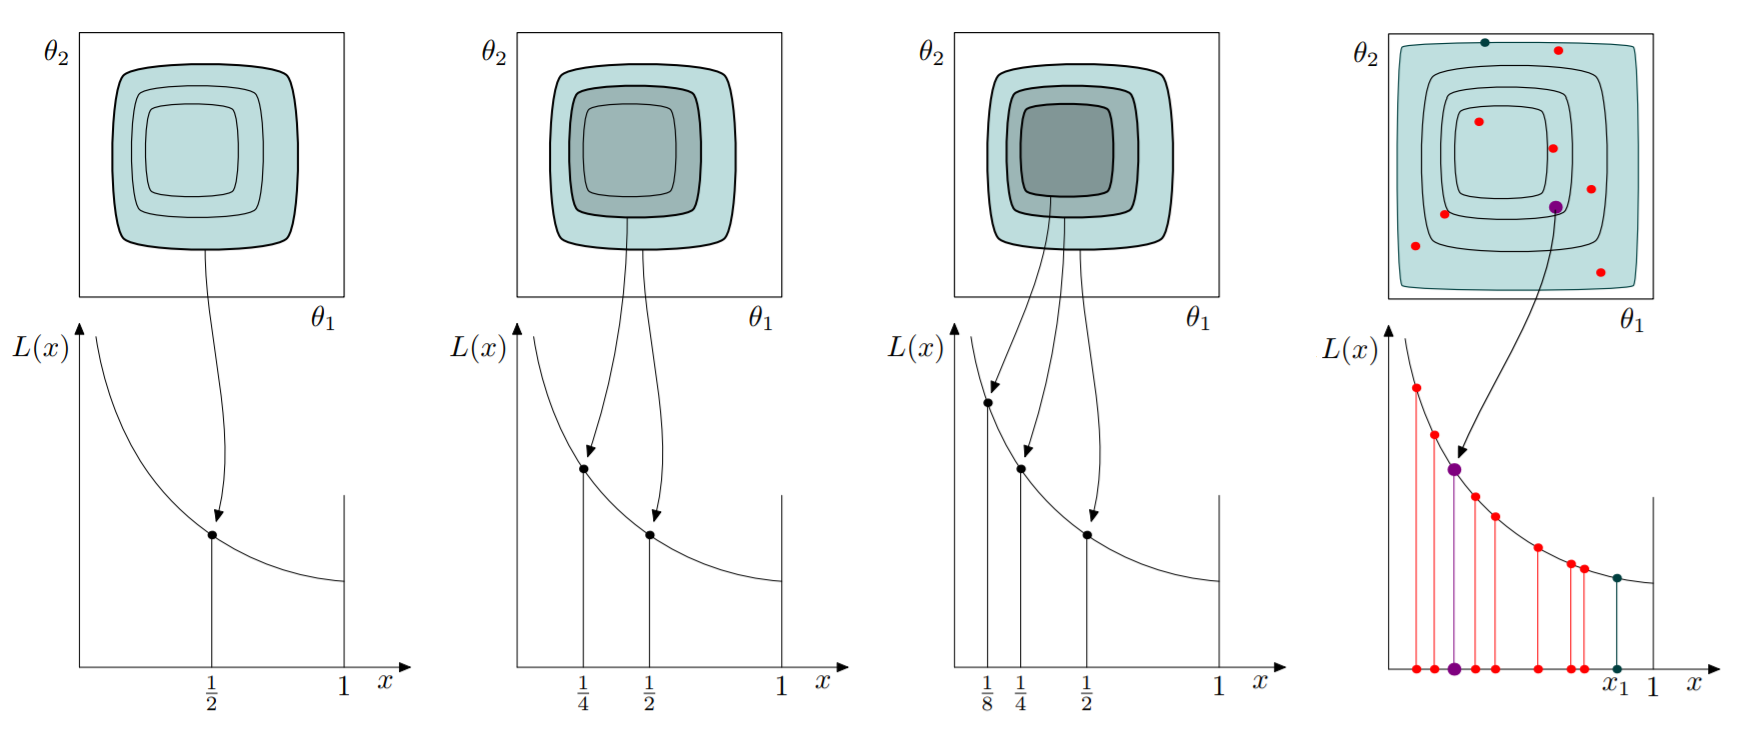
\includegraphics[width=\textwidth]{figures/nested_sampling.png}
    \caption{A visualization of the nested sampling algorithm. Plots along the top represent contour plots of a likelihood function. Bottom plots show likelihood, $L(x)$\,, vs prior mass, $x$. Initially, points are selected uniformly from the prior. Points with the largest likelihoods enclose the smallest prior masses. During each iteration of the sampling, the point with the lowest likelihood ($x_{1}$ in rightmost plot) is replaced via MCMC by a new point uniformly distributed between $0$ and $x_{1}$\,. This shrinks the prior mass and converges upon the best solution. Plots reproduced from \cite{nested_sampling}.}
    \label{fig:nested_sampling}
\end{figure*}
where $P$ represents the posterior mass. $H$ can be said to represent the amount of information in the posterior relative to the prior. Eventually, the likelihoods of the live points will be maximized and each iteration of the nested sampling will provide minimal improvement. At this point the evidence has been sufficiently calculated and the sampling must stop. This is implemented in the code as a cutoff when $i > mH\,$, where $i$ is the number of iterations, $m$ is the number of live points, and $H$ is the information. When this point is reached, the signal and noise evidences have been calculated and SMEE outputs its final result, a signal vs. noise Bayes factor,
\begin{equation}
    \begin{split}
    \log B_{S,N} =& \log[p(D|M_{S})] - \log[p(D|M_{N})] \\
    =& \log Z_{S} - \log Z_{N}
    \end{split}
\end{equation}

After running SMEE with two different sets of PCs, we will have two Bayes factors, each representing a model. A final Bayes factor comparing these two models can be constructed with simple subtraction,
\begin{equation}
\label{equ:model_selection}
    \begin{split}
    \log B_{S_{1},S_{2}} =& \log B_{S_{1},N} - \log B_{S_{2},N} \\
    =& (\log Z_{S_{1}} - \log Z_{N}) - (\log Z_{S_{2}} - \log Z_{N}) \\
    =& \log Z_{S_{1}} - \log Z_{S_{2}}
    \end{split}
\end{equation}
When $\log B_{S_{1},S_{2}} > 0\,$, model $S_{1}$ is preferred, and when $\log B_{S_{1},S_{2}} < 0\,$, model $S_{2}$ is preferred. A confidence threshold, $C\,$, will typically be set on the final Bayes factor. When,
\begin{equation}
\label{equ:confidence_threshold}
    \left|\log B_{S_{1},S_{2}}\right| \geq C
\end{equation}
then the preferred model can be selected with confidence. A reliable confidence threshold can be determined through experimentation, but typical values are in the range of 3-10\,.

\section{Posterior Distributions}

\begin{figure*}[p]
    \centering
    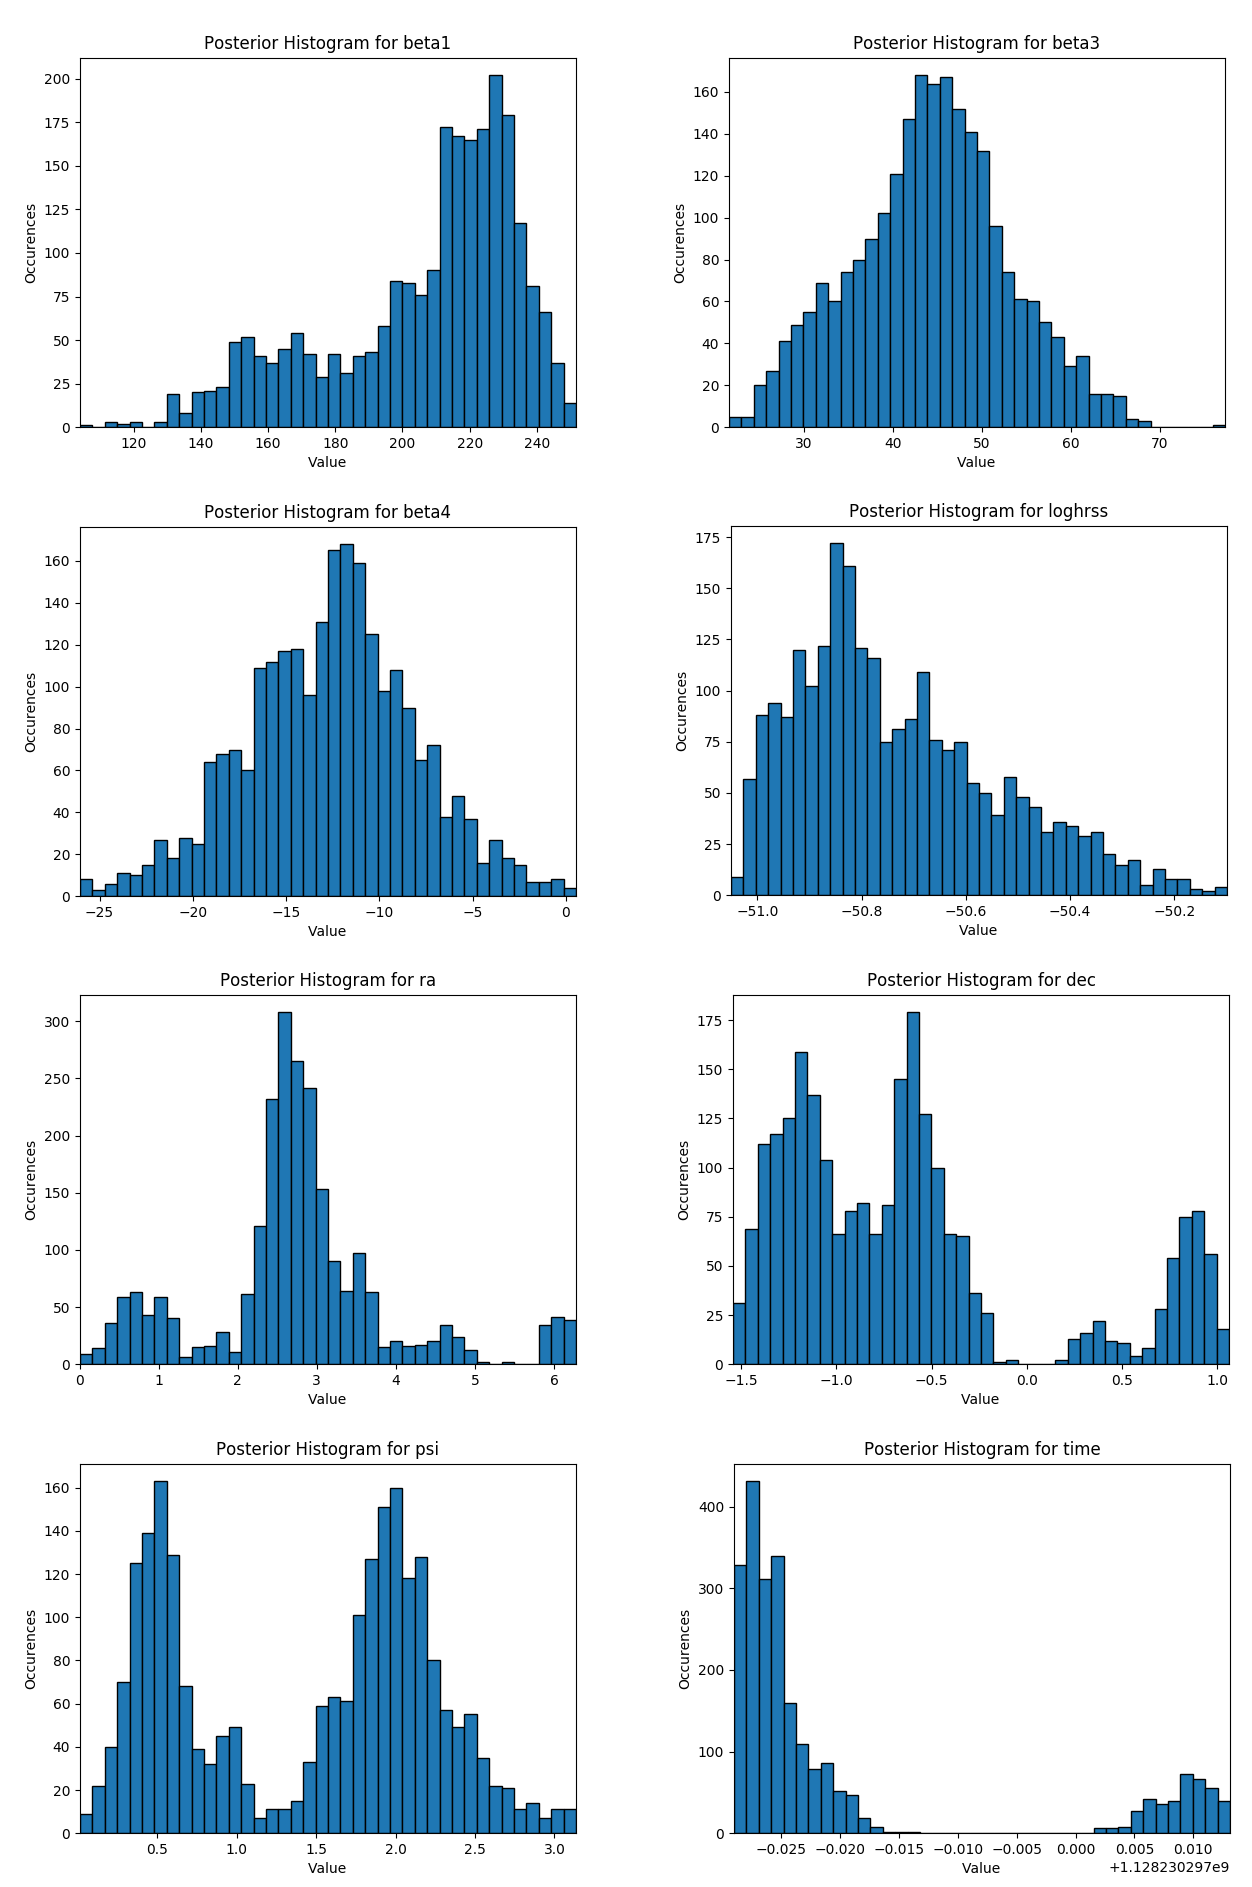
\includegraphics[width=5.1in]{figures/posteriors.png}
    \caption{Posterior distributions for a sample of SMEE's parameters. Betas refer to PC coefficients. Sky localization, represented by right-ascension (ra), declination (dec), and psi, is limited by the fact that SMEE only reconstructs one GW polarization. For most CCSN it is expected that the sky position will be known.}
    \label{fig:posteriors}
\end{figure*}

The Bayes factor is the primary output of SMEE, but a posterior distribution is also produced for each parameter. These parameters include the PC coefficients, the signal $h_{rss}$, the arrival time (center earth), and the sky position. When producing a reconstruction, the maximum likelihood data point is used. This is the last data point produced during nested sampling, as shown in Figure~\ref{fig:nested_sampling}.

Figure~\ref{fig:posteriors} contains example posterior distributions for an injected CCSN waveform. It is possible for SMEE to determine the sky location when not previously known, but the effectiveness of this is somewhat limited by the fact that SMEE only reconstructs one polarization of the signal. For most CCSN signals it is expected that a sky location will be known through electromagnetic and neutrino observations.

\section{Signal Model Catalogs}

\begin{figure*}[p]
    \centering
    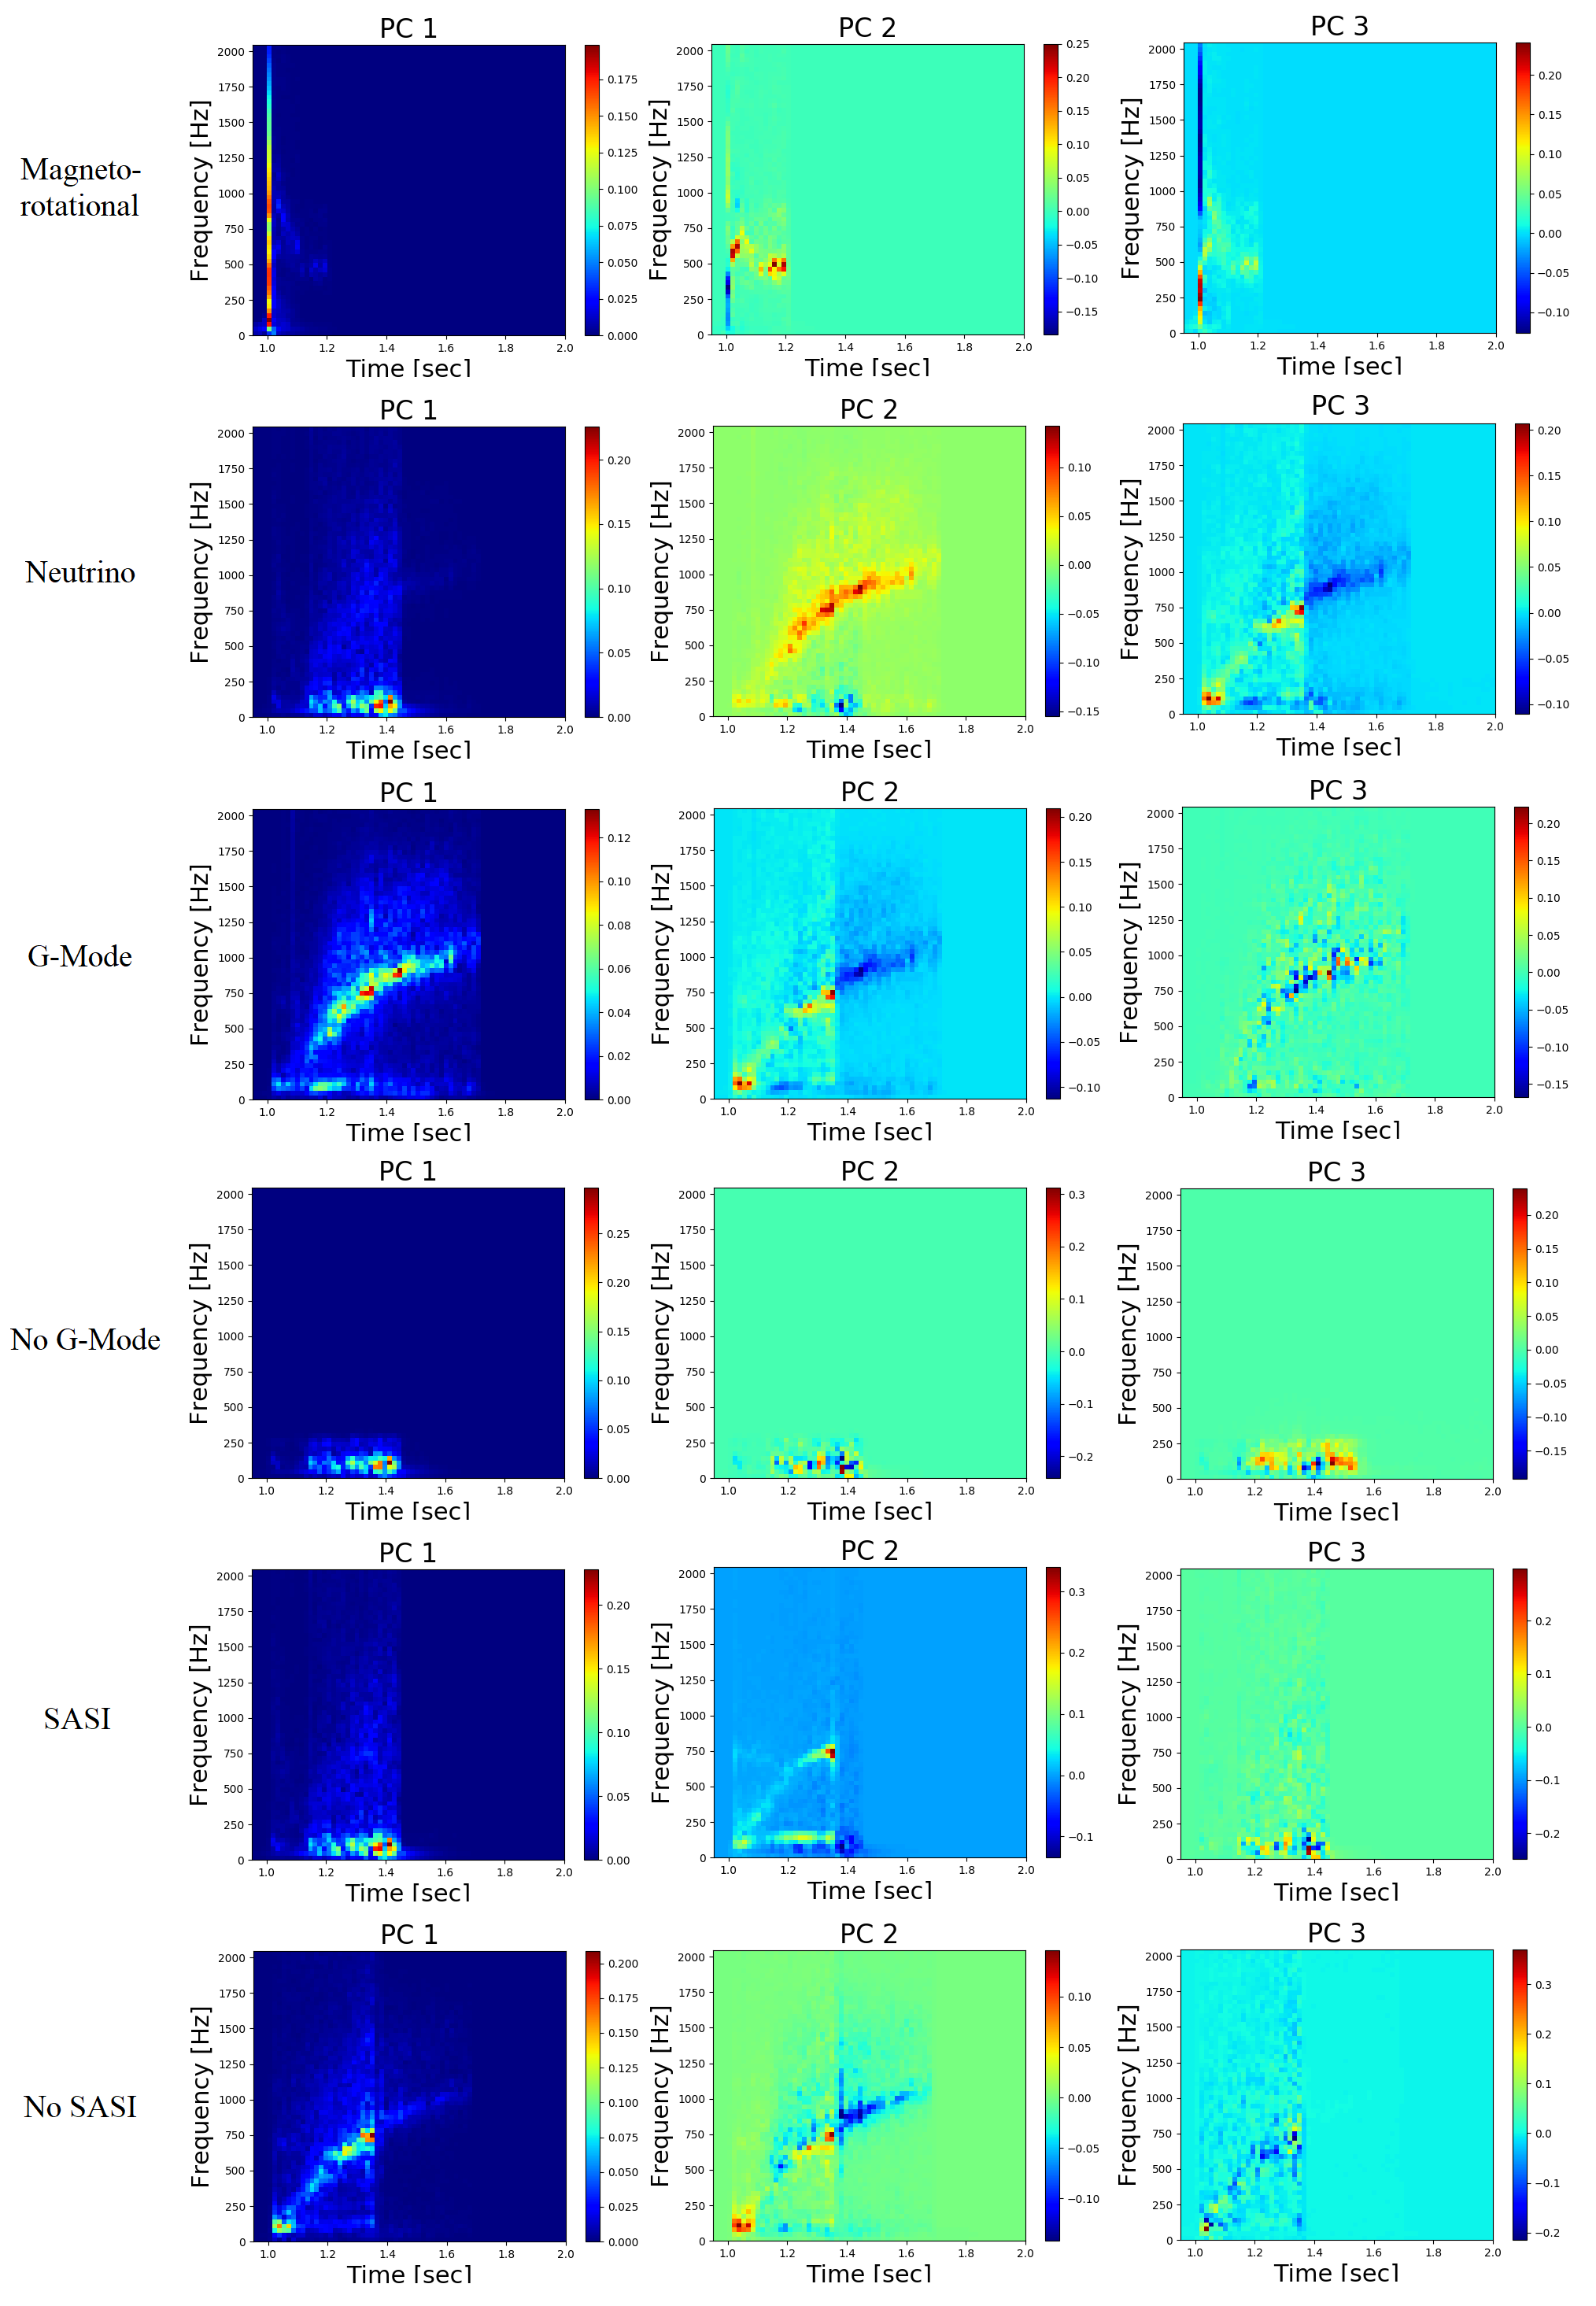
\includegraphics[width=5.5in]{figures/all_PCs.png}
    \caption{The first three PCs for each catalog. From top to bottom, the catalogs are: neutrino mechanism, magnetorotational mechanism, g-modes, no g-modes, SASI, and no SASI. Two catalogs are compared to each other for each classification statement.}
    \label{fig:all_PCs}
\end{figure*}

The first classification statement that SMEE makes is a determination of the explosion mechanism. After core bounce, the stalled shock front must be re-energized in order to successfully cause a supernova explosion. As described in section~\ref{sec:mechanisms}, simulation groups have settled upon two main models to explain this re-energization, the neutrino model for non or slowly-rotating progenitors~\cite{mueller:e12, kuroda:16, andresen:16}, and the magnetorotational model for rapidly-rotating progenitors~\cite{scheidegger:10b, scheidegger2010gravitational}. A signal catalog can be constructed for each model with waveforms of that type. These catalog waveforms will typically come from multiple simulation groups. Each signal catalog produces a set of PCs (as seen in Figure \ref{fig:all_PCs}) that can then be used with SMEE to produce a signal vs noise Bayes factor. Those Bayes factors can then be compared to each other via subtraction to produce a final signal model vs signal model Bayes factor, as in equation \ref{equ:model_selection}. This result tells us which explosion mechanism is more likely for the observed CCSN signal.

The other two classification statements that SMEE makes are related to the presence of predicted features (SASI and g-modes) in the GW signal. As described above, in order to make a statement about the CCSN re-energization mechanism two different sets of PCs had to be used. Each set corresponds to a signal model and the two resulting Bayes factors can then be compared. We follow a similar procedure for waveform feature statements, with one catalog consisting of waveforms that possess the feature and one catalog consisting of waveforms that do not possess the feature (as seen in Figure \ref{fig:all_PCs}). The ``g-mode" Bayes factor, for example, can then be compared to the ``no g-mode" Bayes factor to determine whether g-modes appear to be present in the signal. The procedure is identical for SASI. It should be noted that only neutrino model waveforms are used in these waveform feature catalogs. These features are usually less prominent in rapidly-rotating simulations as the tremendous rotation can suppress convective motion~\cite{2016arXiv160501785A, scheidegger:10b}. Because all of these waveforms are neutrino model waveforms, the performance difference between competing signal model reconstructions can be subtle. Low SNR situations in which only part of the signal is detectable can also be problematic as waveform features can be lost in the noise. This can lead to a higher confidence threshold in equation \ref{equ:confidence_threshold} to ensure good performance for quiet signals.

\section{Number of Principal Components}

\begin{figure*}[t!]
    \centering
    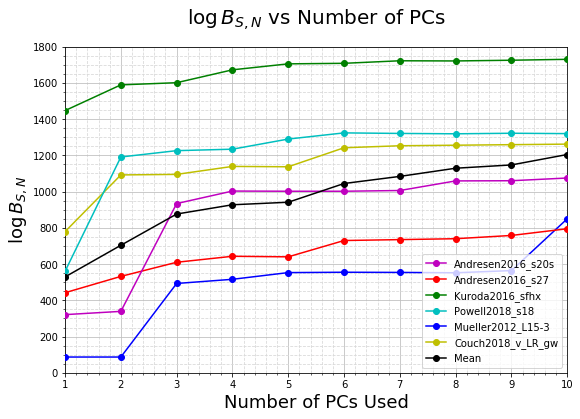
\includegraphics[width=2.9in]{figures/PCs_neu_review.png}
    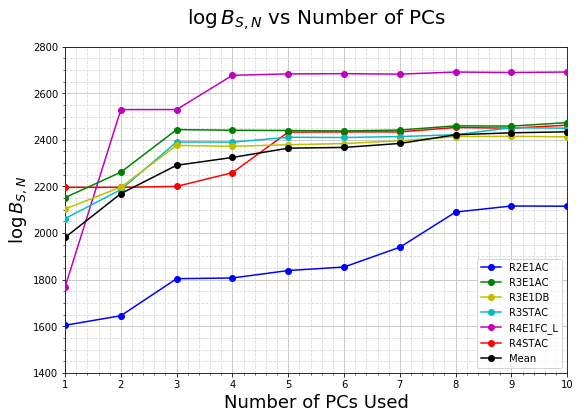
\includegraphics[width=2.9in]{figures/PCs_sch_review.png}
    \caption{Log Bayes factors for mechanism classification with an increasing number of PCs in simulated aLIGO Gaussian noise. Waveforms with a * were not included when making the PCs. The left figure shows neutrino catalog waveforms, and the right figure shows magnetorotational catalog waveforms. 6 PCs for the neutrino model and 5 for the magnetorotational model would be acceptable choices as there is limited $\log B_{S,N}$ improvement beyond those points.}
\label{fig:pick_pcs}
\end{figure*}

The number of PCs used can vary within SMEE. In general, the reconstructions will improve at a diminishing rate as more PCs are included. Figure~\ref{fig:pick_pcs} shows this for mechanism classification PCs. Naturally it is desirable to find a number of PCs that can sufficiently reconstruct every catalog waveform, but Bayesian inference tends to prefer simpler models, especially in low SNR cases, due to the Occam factor~\cite{mackay2003information, thesis_jade}. Models with large numbers of parameters can predict a larger number of data sets and the confidence of individual results suffers a penalty. Figure~\ref{fig:pick_pcs} was produced by injecting CCSN waveforms into Gaussian data with an SNR of 20. The number of PCs can also be chosen by setting a threshold on the explained variance, defined in equation~\ref{equ:variance}.
\chapter{SMEE Performance}
\label{chp:performance}

This chapter will summarize the performance of SMEE as a parameter estimation tool. A sample of results from SMEE's code review will be presented, an example case study will be performed, and future detector configurations will be simulated in order to gauge how SMEE's performance will improve over the coming decades.

\section{SMEE Code Review}

SMEE is currently under review in order to be added to LIGO's official run plan for GW signals from CCSNe. Different aspects of SMEE's algorithm have been tested and some of those results will be presented in this section.

As discussed in section~\ref{sec:PCA}, performing PCA on spectrograms means chopping up the columns of a spectrogram, combining those columns into one long vector, running the PCA algorithm on said vector, and then reassembling everything back into a spectrogram for later use. The first simple test was to examine the effects of reordering the columns before PCA. In short, this had no effect on the PCs produced. As long as the PC vector was chopped up and reassembled in a consistent fashion (so that the final spectrogram was in the proper order), there was no discernible impact on the PCs. The original PCs and the reordered PCs also produced identical Bayes factors for identical injections.

\begin{figure*}[t!]
\centering
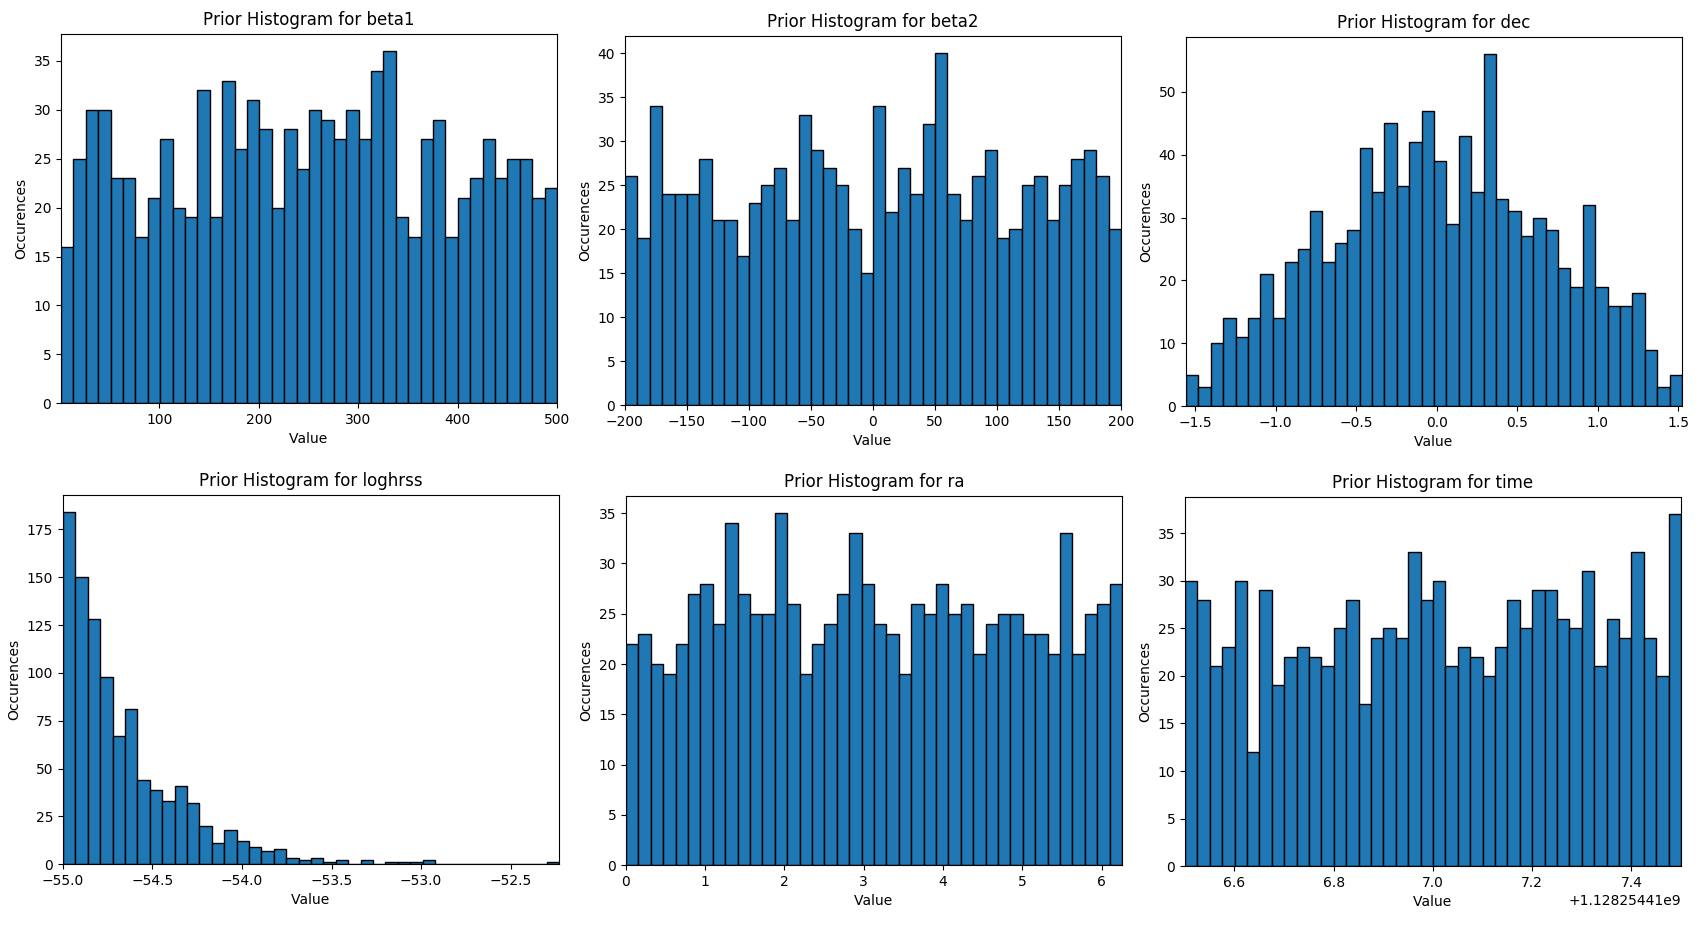
\includegraphics[width=\textwidth]{figures/priors.png}
\caption{Six prior distributions within SMEE. The prior for declination is uniform in cosine, the prior for $\log h_{rss}$ is uniform in volume, and the remaining priors are flat.}
\label{fig:priors}
\end{figure*}

The prior distributions within SMEE were also tested and can be seen in Figure~\ref{fig:priors}. Most of SMEE's parameters have a flat, uniform prior distribution. SMEE's priors are discussed in section~\ref{sec:priors}. The priors behaved as expected when tested.

The performance of SMEE when running on noise (no CCSN signal) is extremely important. CCSN searches are typically triggered by electromagnetic and neutrino observations. A window of data is then selected to represent the possible arrival time of a GW. This window is searched for excess power events that are coherent between detectors. It is important that SMEE does not see CCSN signals in the data when they are not genuinely present. To test this, SMEE was ran 1000 times on randomly chosen segments of O1 data. This was performed with the neutrino and magnetorotational PCs. All of these trials produced negative $\log B_{S,N}$ values, indicating that no signals were detected. These results are shown in Figure~\ref{fig:noise_runs}.

\begin{figure*}[t!]
\centering
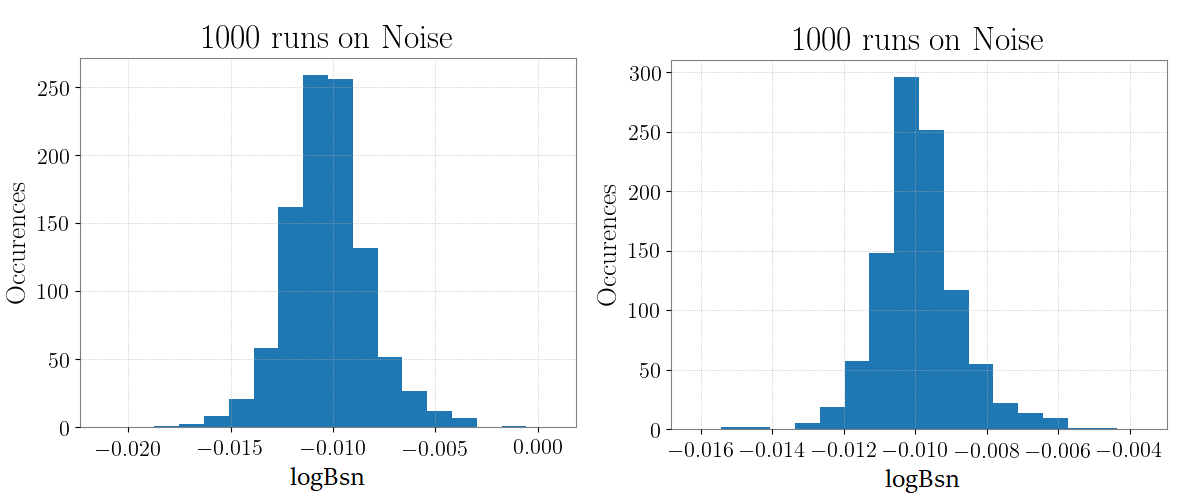
\includegraphics[width=\textwidth]{figures/noise_runs.png}
\caption{Left: Noise performance with Neutrino model PCs. Right: Magnetorotational PCs. All tests were performed on O1 data with no injections.}
\label{fig:noise_runs}
\end{figure*}

\section{Reconstructions}

This section contains example SMEE reconstructions with different sets of PCs. All injections were performed from 3\,-\,5\,kpc with a known sky position into a simulated future detector configuration with two A+ detectors, one Advanced Virgo detector, and one Kagra detector. For the mechanism classification reconstructions, all injections were non-catalog waveforms. This was not the case for waveform feature classification due to a limited number of waveforms.

\begin{figure*}[p]
    \centering
    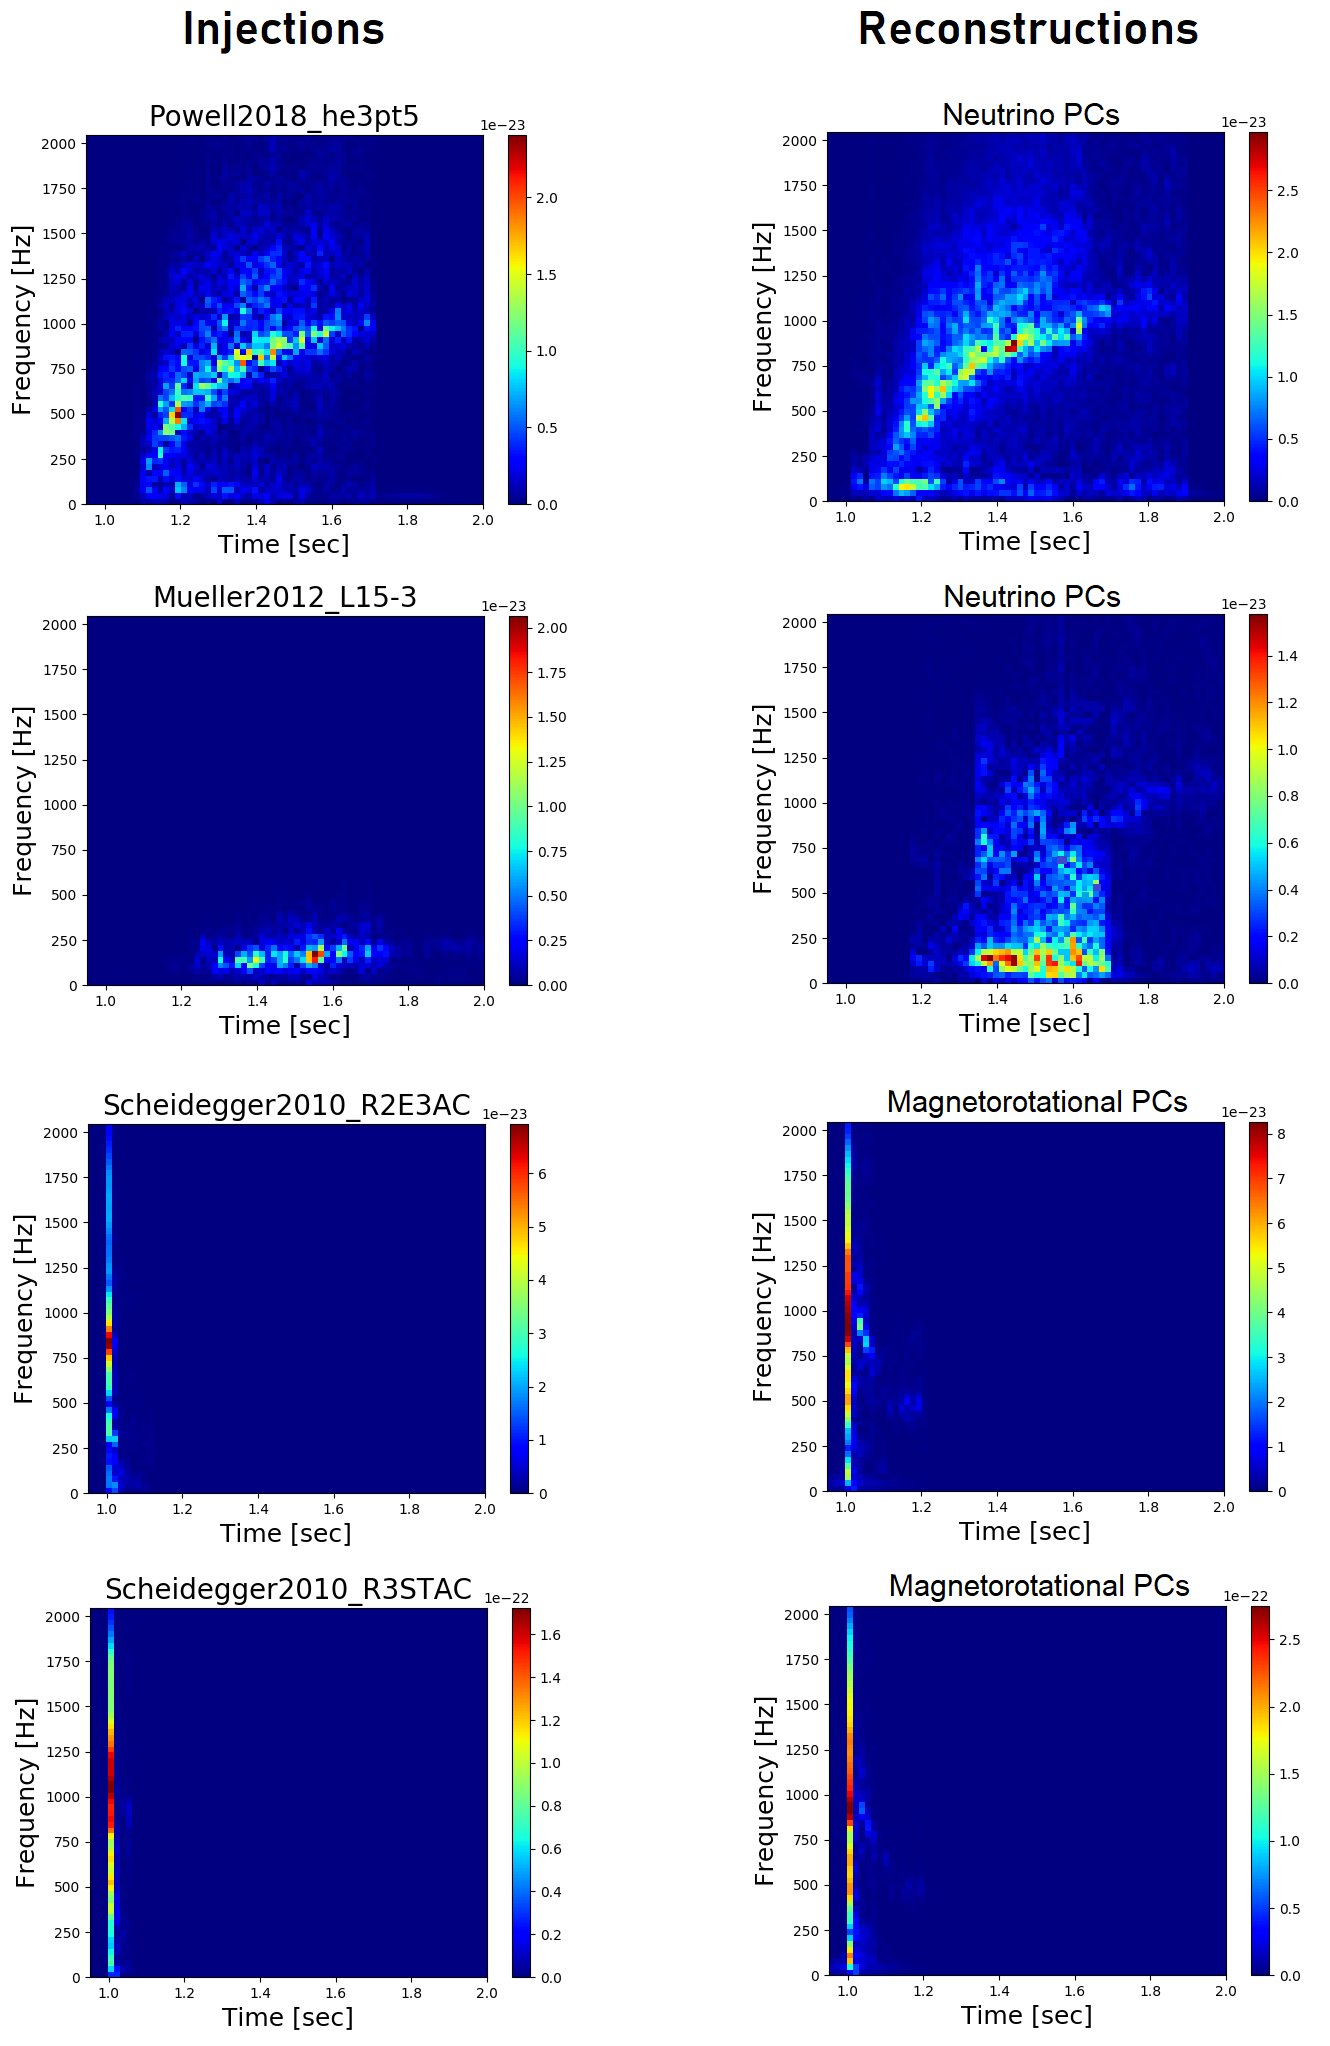
\includegraphics[height=8.3in]{figures/mechanism_reconstructions.png}
    \caption{Example reconstructions for mechanism classification PCs.}
    \label{fig:mechanism_reconstructions}
\end{figure*}

\begin{figure*}[p]
    \centering
    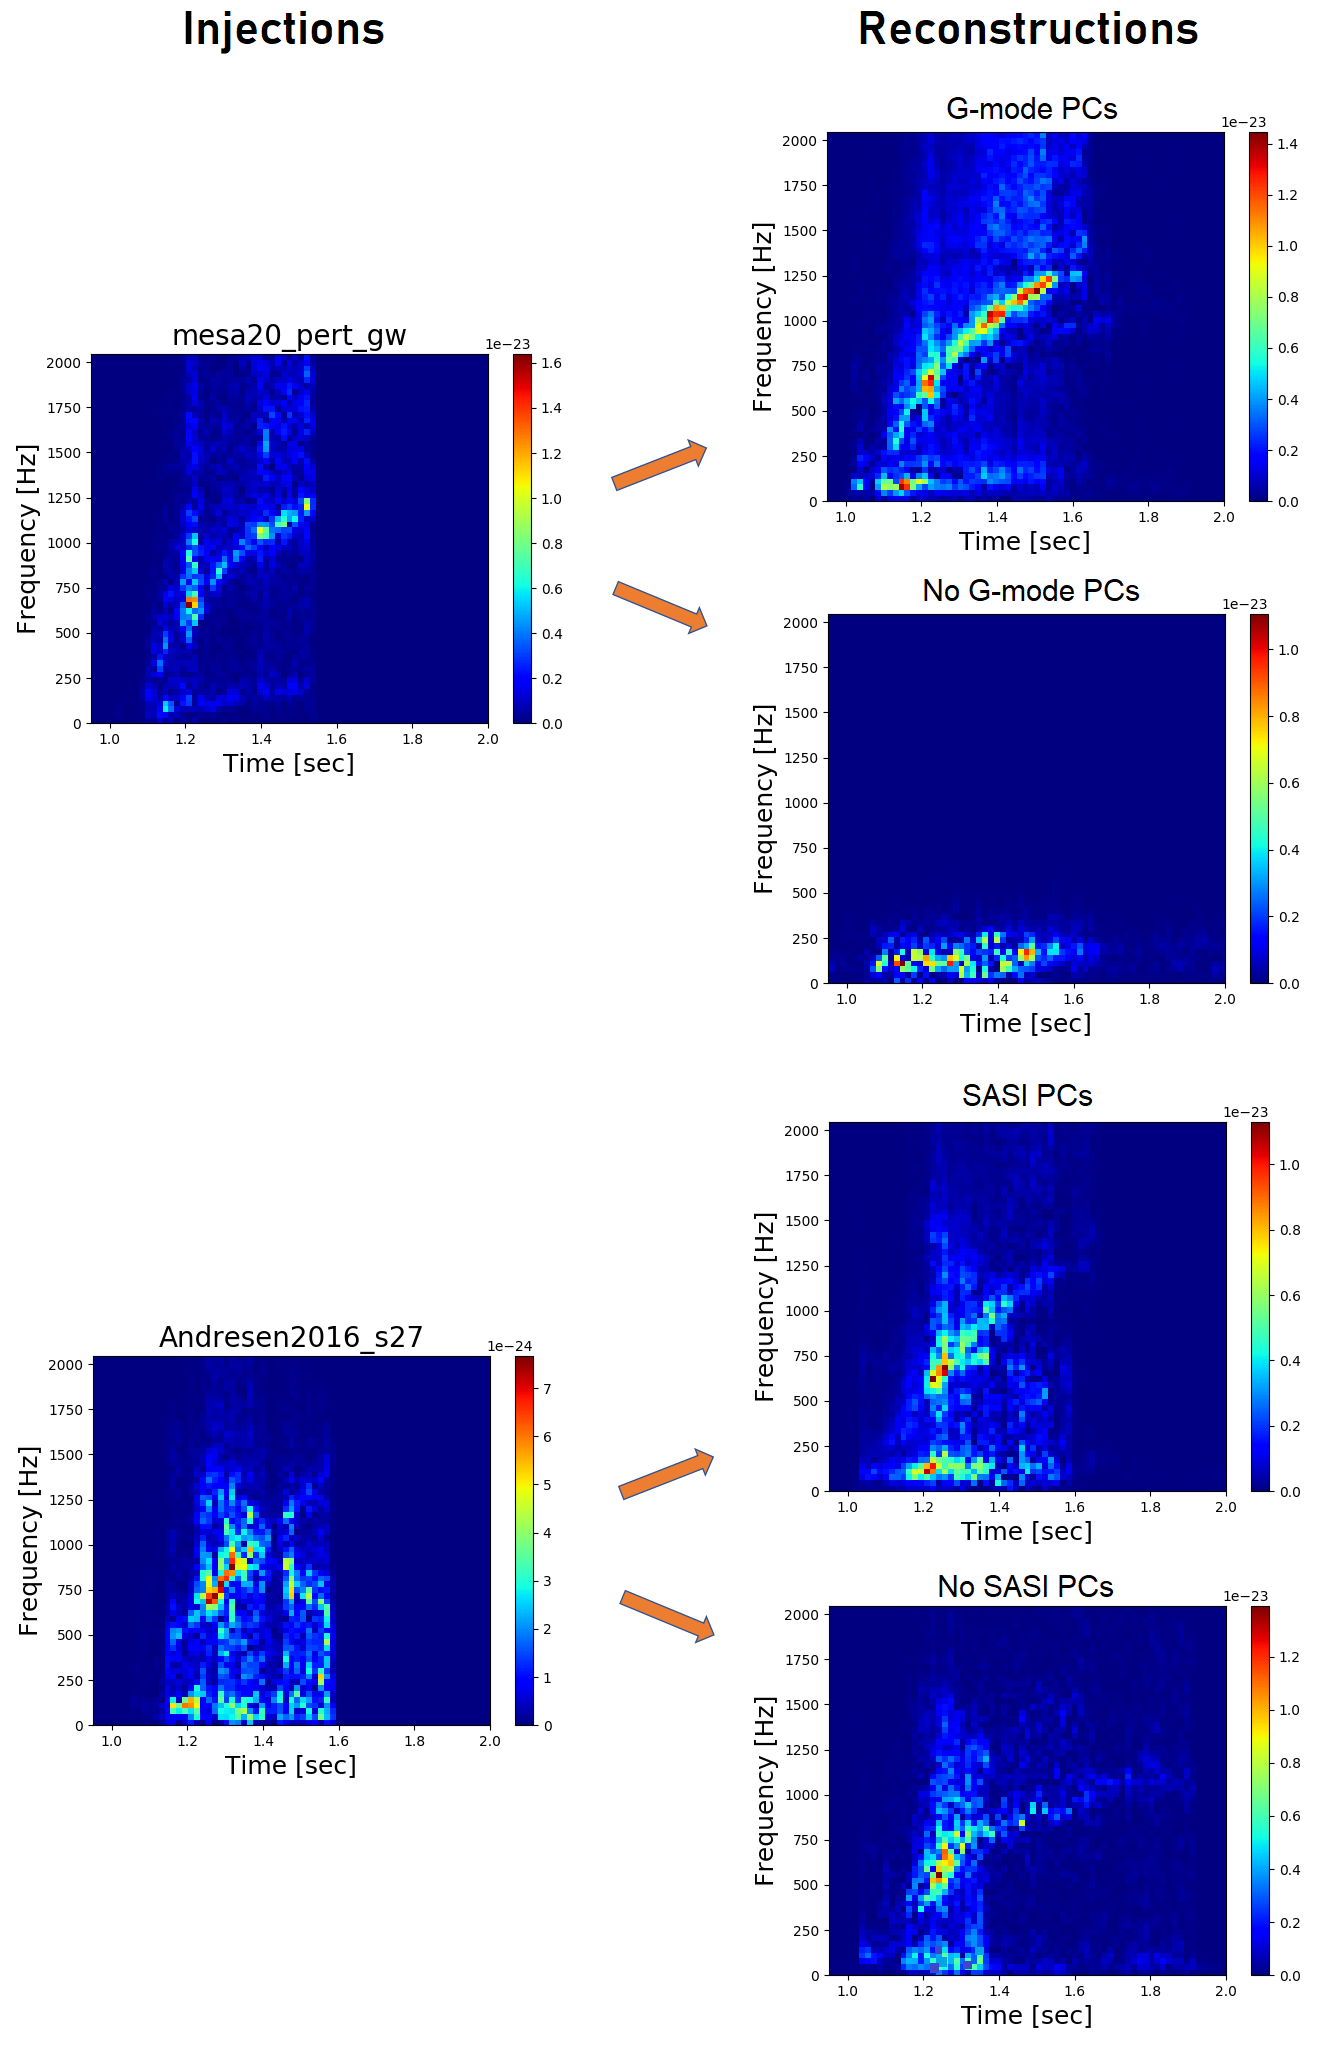
\includegraphics[height=8.3in]{figures/feature_reconstructions.png}
    \caption{Example reconstructions for waveform feature classification PCs.}
    \label{fig:feature_reconstructions}
\end{figure*}

Reconstructions with mechanism classification PCs are shown in Figure~\ref{fig:mechanism_reconstructions}. Reconstructions with waveform feature PCs are shown in Figure~\ref{fig:feature_reconstructions}. For the mechanism classification PCs, only reconstructions with the ``correct" PCs, the PCs that match the injection type, are displayed. All injections reached the Bayes factor threshold for confident classification.

\section{Example Case Study}

\begin{figure*}[b!]
\centering
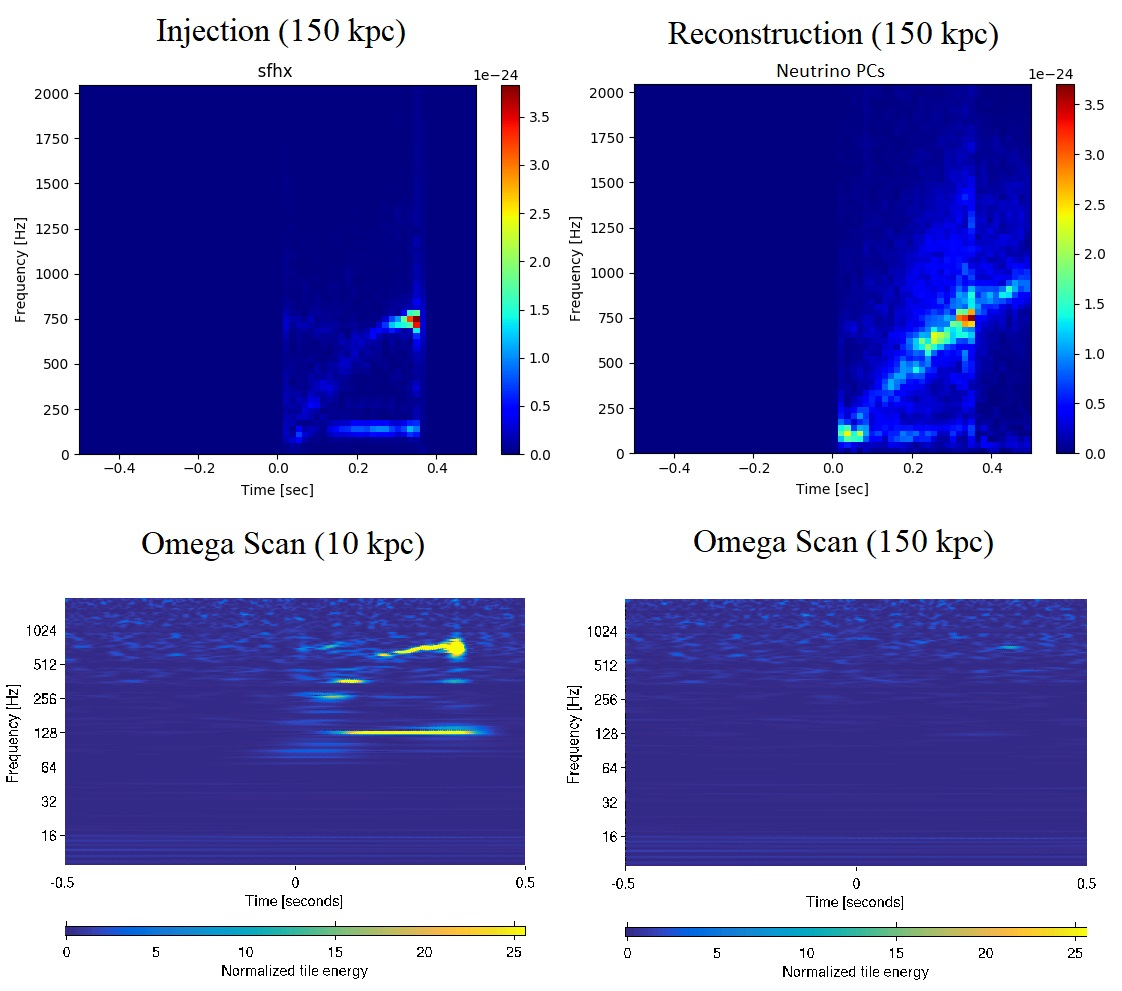
\includegraphics[width=15cm]{figures/Reconstruction_Plot_8.jpg}
\caption{Top row shows injected waveform and waveform reconstruction produced with the neutrino model PCs at 150\,kpc in three ET and two Voyager detectors. Bottom row shows Omega Scan spectrograms of the data from the detector in the configuration with the highest SNR. Bottom left plot shows the signal is clearly visible by eye for a 10\,kpc injection (SNR = 120), while the bottom right plot shows almost nothing visible at 150\,kpc (SNR = 8). This waveform was confidently classified at 150\,kpc as corresponding to the neutrino model with g-mode and SASI emission, even though at that distance those features are clearly not visible by eye in the noisy Omega scan.}
\label{fig:recon}
\end{figure*}

This section will summarize an example case study in which model sfhx was injected into a simulated configuration with three ET detectors and two Voyager detectors. The signal was injected at a distance of 150\,kpc using an arbitrary sky position. The resulting network SNR was 11.4\,. The injected waveform, an example reconstruction, and example Omega Scans of one detector's data are shown in Figure~\ref{fig:recon}. Omega scans are commonly used spectrograms to view detector data within the LIGO collaboration~\cite{chatterji2004multiresolution}. All three classification statements were performed on the signal. With the neutrino model PCs, the result was $\log B_{S,N} = 55.5\,$. With the magnetorotational PCs the result was $\log B_{S,N} = 1.5\,$. This gives a final mechanism classification result of $\log B_{neu,mag} = 54\,$. This result is well above the confidence threshold and tells us that our signal matches the neutrino model much more strongly than the magnetorotational. Because it appears to be a slowly rotating neutrino model waveform, the two waveform feature classification statements can be performed.

For g-mode and SASI classification, the g-mode PCs gave a result of $\log B_{S,N} = 62.7\,$, while the no g-mode PCs gave $\log B_{S,N} = 1.3\,$. Subtracting the two gives the final g-mode result of $\log B_{gmode,\,no\,gmode} = 61.4\,$. This is also well above the confidence threshold and tells us strongly that high frequency g-modes were present in the signal. The SASI PCs gave a result of $\log B_{S,N} = 97.7\,$ while the no SASI PCs gave $\log B_{S,N} = 61.8\,$. This gives the final result for SASI classification, $\log B_{SASI,\,no\,SASI} = 35.9\,$. This is also above the confidence threshold and tells us that low frequency SASI signals were present in the data. For this simulated CCSN signal, all three classification statements were made with a high confidence level even though the network SNR of the signal is relatively low and the signal features are clearly not visible in the noisy spectrogram shown in Figure~\ref{fig:recon}. % When the same model is injected with an SNR of 23, at half that distance considered in this example, almost the entire waveform is still not visible in an Omega Scan of the detector data.

\section{Minimum SNR}

\begin{figure*}[b!]
\centering
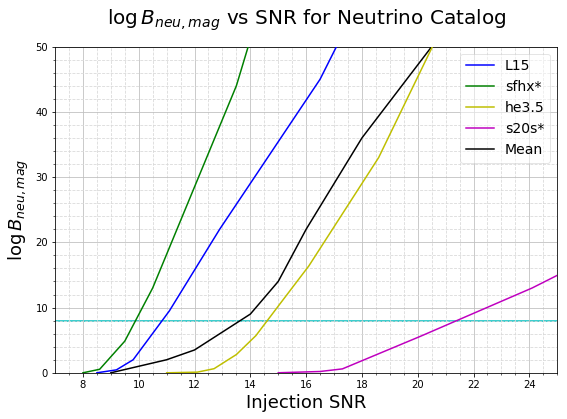
\includegraphics[width=2.75in]{figures/SNR_neu.png}
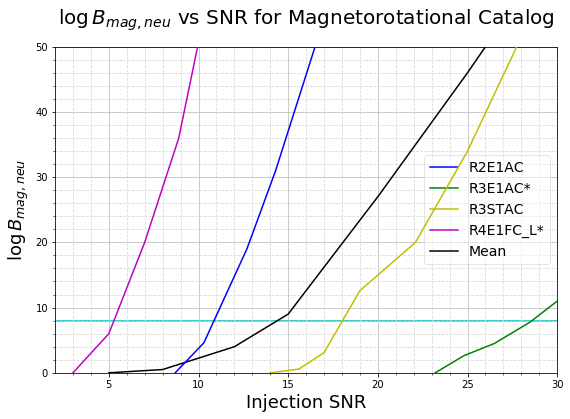
\includegraphics[width=2.75in]{figures/SNR_sch.png}
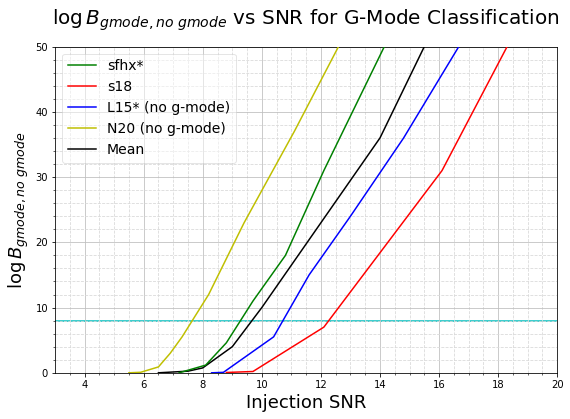
\includegraphics[width=2.75in]{figures/SNR_gmode.png}
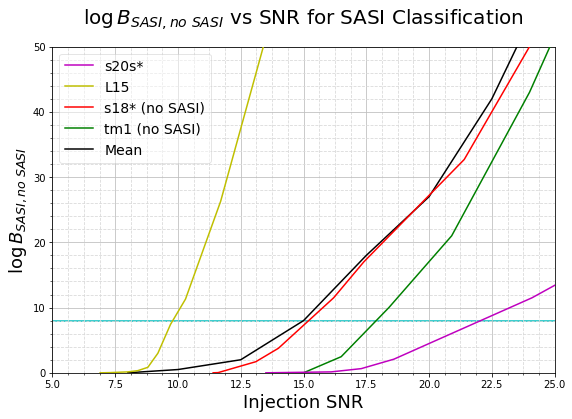
\includegraphics[width=2.75in]{figures/SNR_sasi.png}
\caption{Minimum detectable SNR for each classification statement. All injections performed in a simulated A+ configuration that included Advanced Virgo and Kagra. The top two plots both pertain to mechanism classification, and the bottom two are for g-modes and SASI. Models with an asterisk (*) were not included in the PCA. All results are organized such that positive Bayes values correspond to correct classifications regardless of whether the feature is present or not.}
\label{fig:min_snr}
\end{figure*}

The top two panels in Figure~\ref{fig:min_snr} show the mechanism classification performance for neutrino and magnetorotational waveforms as a function of injected network SNR. All SNR plots were created while running SMEE on a simulated A+ configuration that will be described in Section~\ref{subsec:eras}. On average, neutrino model waveforms needed an SNR of about 14 or greater to be confidently classified. Some waveforms, such as s20s, required an SNR in the low twenties. This is likely due to the fact that this waveform's peak frequency of emission is around 100\,Hz and the short PSDs in SMEE's spectrograms are hindered by the 60\,Hz mains power peak present in Advanced LIGO's data. This can lower our sensitivity to signal energy in the vicinity of 60\,Hz. Magnetorotational waveforms performed similarly and also had an average minimum SNR of about 14, with one plotted waveform requiring an SNR above 28. Despite the similar minimum SNRs, magnetorotational waveforms are generally easier to resolve at a given distance due to their larger signal energies. 

The bottom two panels in Figure~\ref{fig:min_snr} show SMEE's performance as a function of SNR for SASI and g-mode classification. The average minimum SNR required to make statements about the presence of g-modes was just below 9, while the average minimum for SASI statements was 15. Similarly to mechanism classification, s20s required the largest SNR of about 22 in order to confidently say that SASI was present. This is, again, likely due to SMEE's hindered sensitivity around 60\,Hz. It was generally similarly difficult for SMEE to determine that a feature was present than to rule it out, with both cases sometimes performing better.

\section{Methodology for Testing Future Detectors}

The analysis presented in this section was designed to test SMEE's effectiveness in future detector arrangements. Specifically, the ability to distinguish between explosion mechanisms (neutrino vs magnetorotational) along with the ability to make statements about the presence of predicted waveform features (SASI and g-modes) in an observed signal. Future detector data is simulated as realistically as possible by adjusting segments of Advanced LIGO's O1 data to match the estimated sensitivity curves of future detectors in a process called ``recoloring". We can then ``inject" a waveform by inserting its time series into the detector data. We inject CCSN waveforms over the entire sky at different GPS-times and with different orientations in order to test SMEE's performance on emissions from an unknown, possibly extra-galactic source. The results of these tests will be presented in section~\ref{sec:performance}.

\subsection{Recoloring}

\begin{figure}[b!]
\centering
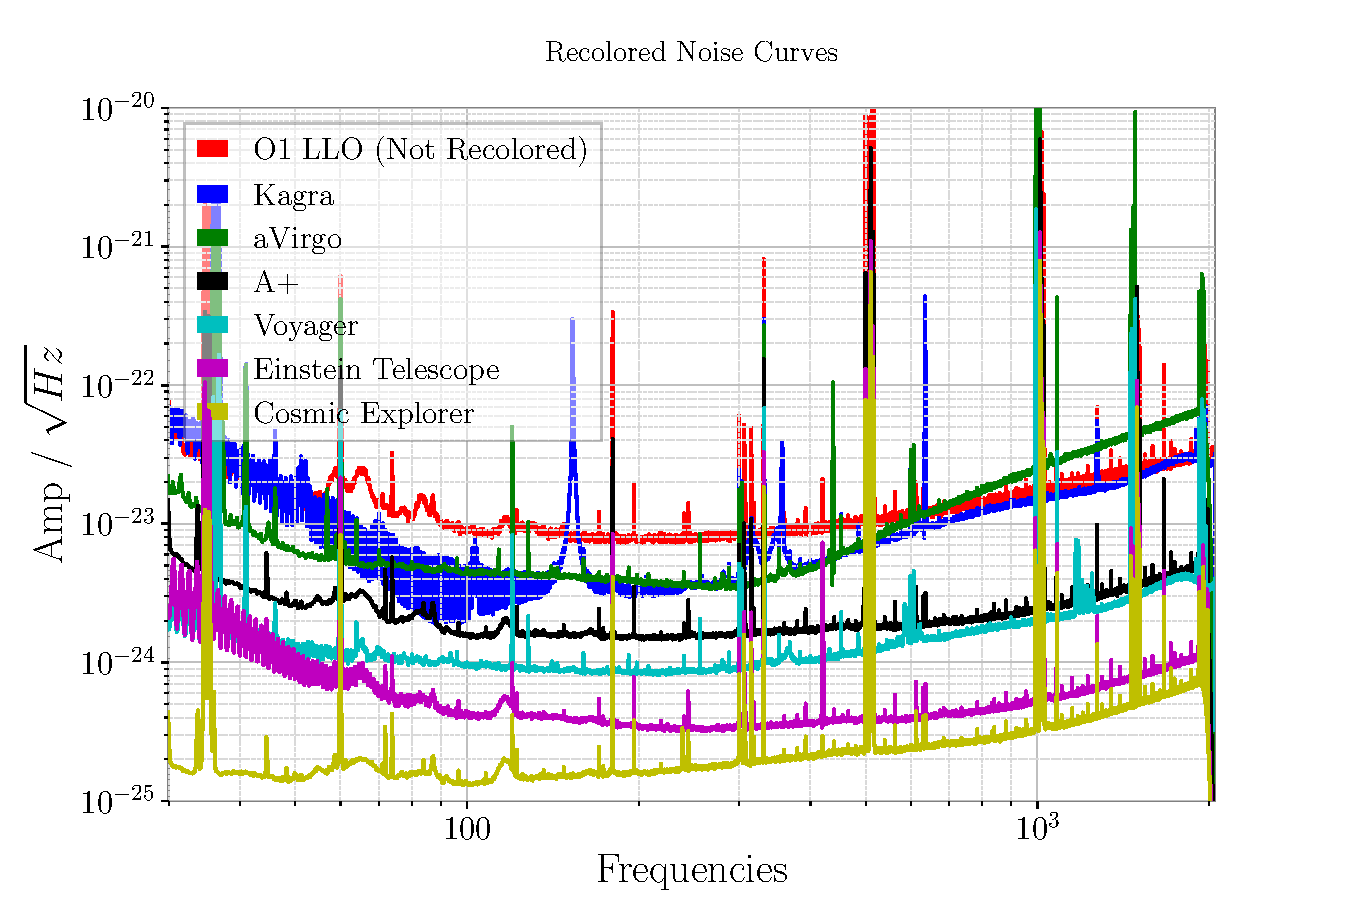
\includegraphics[width=\textwidth]{figures/recolored_noise_curves.pdf}
\caption{Spectra for LIGO O1 data recolored to future detector sensitivities. Data is shown from 30 - 2048 Hz, the frequency band used in SMEE's analysis.}
\label{fig:recolored_curves}
\end{figure}

Six different 24 hour segments of data from Advanced LIGO's first observing run (O1) were chosen to be recolored. Recolored data possesses the calibration lines and transient noise glitches not found in simulated Gaussian data. The recoloring was performed with the GSTLAL software package~\cite{messick2017analysis}. GSTLAL contains software for data manipulation and the generation of simulated data. In this case, each segment of data was whitened with a reference PSD and then recolored with a filter to the noise curves of future detectors. The noise curves for the recolored data are shown in Figure~\ref{fig:recolored_curves}. Cosmic Explorer is the most sensitive detector considered in this study. After recoloring, each segment of data was reassigned to start at GPS time 1128211934. One segment of data, starting at 1132759948, contained O1 data from Livingston, while the other five (epochs: 1128211934, 1135238505, 1128618400, 1129037417, 1130767217) contained data from Hanford. All of the O1 data used is available from the Gravitational Wave Open Science Center (GWOSC)~\cite{2015JPhCS.610a2021V}.

\subsection{Detector Eras}
\label{subsec:eras}

Future detector configurations have been simulated over the next few decades. All predicted dates of operation are rough estimates that may change significantly. The first configuration consists of LIGO A+ (2), Advanced Virgo, and Kagra. Advanced Virgo is already operational and will join the two Advanced LIGO detectors for the next Observing Run in 2019~\cite{AdVirgo}. Kagra is also expected to come online in the near future and may participate in O3~\cite{2013PhRvD..88d3007A, Somiya2012detector, aso2013interferometer}. The funding for LIGO A+ has been approved and this three detector configuration should be operational by approximately 2022. The second configuration is similar but upgrades each LIGO detector. It has LIGO Voyager (2), Advanced Virgo, and Kagra. These detectors are expected to be operational between the period of 2024\,-\,2028. The third configuration is identical but adds a third Voyager detector located in India. An interferometer is planned for India~\cite{unnikrishnan2013indigo} but it is unknown precisely what technology will be included or what sensitivity it will have upon arrival.

The fourth configuration consists of the triangular Einstein Telescope (3) in Europe and two Voyager detectors at the current LIGO sites. The Einstein Telescope represents the first truly 3rd Generation detector~\cite{0264-9381-27-19-194002, ET:design}. Because it is a triangular detector, the single site will operate three interferometers. The Einstein Telescope may be operational by 2027. The fifth and final configuration consists of Cosmic Explorer and the Einstein Telescope (3). This configuration contains only 3rd Generation detectors and will require LIGO to obtain a new construction site as neither current location is large enough for the 40\,km arms~\cite{2017CQGra..34d4001A, whitepaper2018}. This configuration may be operational by $\sim2037$ but will depend on many factors.

\subsection{Injection and Sky Patterns}

Previous SMEE papers have examined performance from galactic sources, usually injecting signals from the galactic center's sky position~\cite{powell:16b, 2017PhRvD..96l3013P}, but future detectors will likely be sensitive to CCSN sources well outside of our own Galaxy~\cite{0264-9381-27-19-194002, 2017CQGra..34d4001A}. Because of this, waveforms are injected from six positions evenly distributed over the entire sky to test performance from an arbitrary source. At each sky location, injections are performed with three different polarization angles (0,\,$\pi/3$,\,$2\pi/3$) evenly distributed throughout the possible parameter space. This is done at five different GPS times evenly distributed throughout a 24 hour period to account for Earth's rotation and the detectors' changing antenna patterns. Injections are performed at 5 GPS times, with 6 different sky locations, and with 3 different polarization angles. That means that for each signal model, each waveform is injected 90 times at each distance. This gives a reasonable sample of results to gauge performance from an unknown source. The injections are performed for each detector era and configuration described in the previous section.

\subsection{Mechanism Classification}

Two waveforms were omitted from the neutrino catalog and the magnetorotational catalog during the creation of the signal models. Any real life CCSN signal we observe will, of course, not identically resemble any simulated waveform in the catalog, therefore these omitted non-catalog waveforms serve as a more realistic test of a genuine signal. For the catalog waveforms (waveforms included in the PCA), four were selected from each catalog and injected as described in the previous paragraphs. For the neutrino catalog, s20s, tm1, C15, and s18 were selected from different simulation groups. All of the magnetorotational waveforms came from the Scheidegger group, so the four chosen, R2E1AC, R3E1DB, R3STAC, and R4STAC, were evenly distributed between the minimum and maximum signal energies of the catalog. We define efficiency at a given distance as the fraction of injected waveforms that could be correctly identified with a log Bayes factor above our confidence threshold. The remaing injections could not be confidently classified. For this analysis, our confidence threshold was $\log B_{i,j} \geq 8$~\cite{powell:16b, 2017PhRvD..96l3013P}.

\subsection{Presence of SASI/G-modes}

Two non-catalog waveforms were injected for each waveform feature. One waveform has the feature and the other does not. The waveforms were injected in the manner described above and the same confidence threshold was used ($\log B_{i,j}~\geq~8$). Regardless of whether the feature was present or not, the Bayes factors will be oriented such that positive answers are the correct answers. As an example, for an injection containing a g-mode signal, $\log B_{gmode,\,no\,gmode}\,$ would be calculated, whereas for an injection containing no g-mode signal, $\log B_{no\,gmode,\,gmode}$ would be calculated. This allows related results to be presented in one simple figure.

\section{Future Detector Performance}
\label{sec:performance}

\subsection{Mechanism Classification}
\label{subsec:mechanism_range}

\begin{figure*}[b!]
\centering
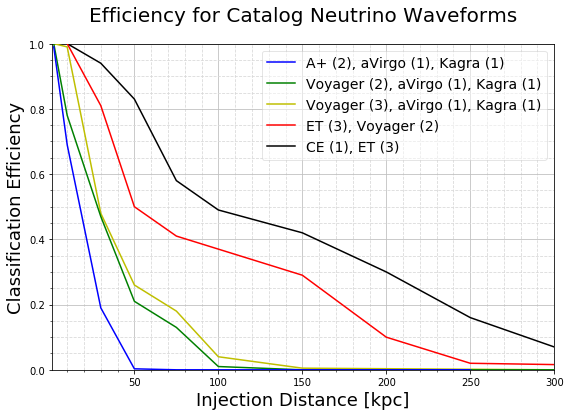
\includegraphics[width=2.75in]{figures/neu_eff_cat.png}
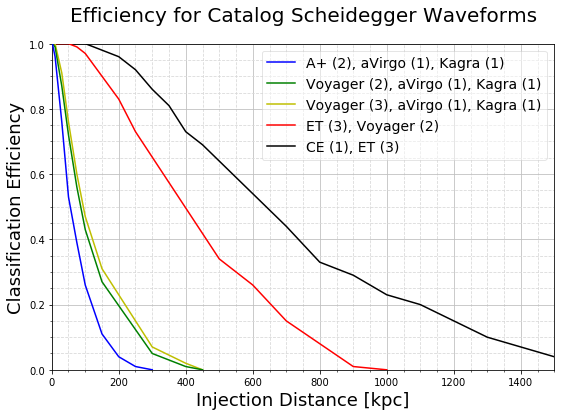
\includegraphics[width=2.75in]{figures/sch_eff_cat.png}
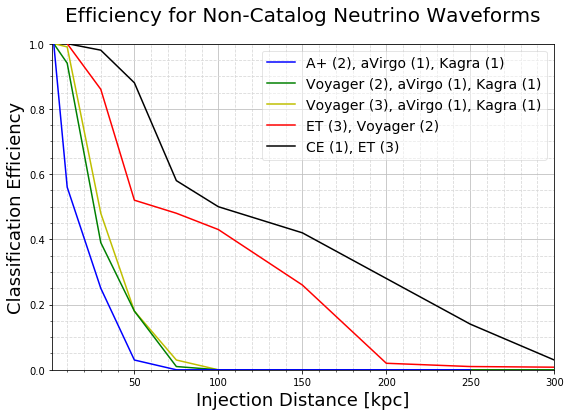
\includegraphics[width=2.75in]{figures/neu_eff_nonc.png}
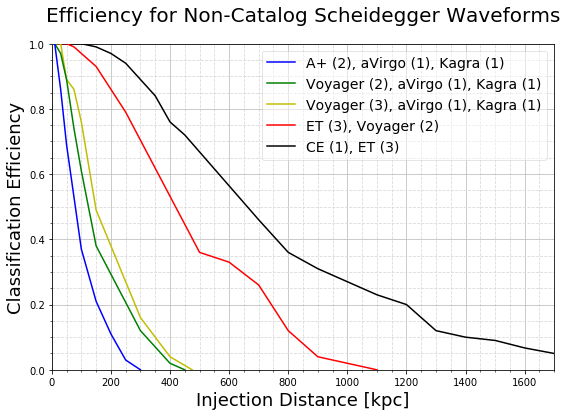
\includegraphics[width=2.75in]{figures/sch_eff_nonc.png}
\caption{Mechanism classification efficiency. Top plots show results for catalog waveform injections, bottom plots show results for non-catalog injections. Non-catalog injections are considered to be the most realistic test case for a genuine gravitional wave signal from an arbitrary source.}
\label{fig:eff_mech}
\end{figure*}

SMEE's ability to determine a source's explosion mechanism is shown in Figure~\ref{fig:eff_mech} for both catalog waveform injections and non-catalog injections. The performance differs greatly when injecting magnetorotational model waveforms vs injecting neutrino model waveforms due to the former having greater energy levels. For both explosion mechanism models, the non-catalog performance is very similar to that of catalog waveforms. The fact that non-catalog performance is on par with catalog performance is a testament to the robustness of SMEE's spectrogram format. 

All future detector arrangements were able to confidently classify magnetorotational injections well beyond the limits of the Milky Way, with the third generation detectors confidently classifying about 50\% of injections at a distance of 400\,-\,700\,kpc and 10\% of injections at a distance of 1.5\,Mpc. For neutrino model waveforms, all future detector arrangements performed with greater than 56\% efficiency at 10\,kpc, suggesting that the explosion mechanism of a galactic CCSN would likely be confidently classified. Low energy explosions, and explosions originating from unfortunate sky positions, could still fail to be classified from within our galaxy in LIGO's A+ configuration. Only 2\,-\,5\% of galactic injections failed to be confidently classified in Voyager configurations. Adding a third Voyager detector improves coverage and efficiencies at close distances, but does little to increase SMEE's range. All galactic injections were confidently classified in the ET and Cosmic Explorer arrangements. Third generation detectors had a 50\% efficiency for neutrino model waveforms at a distance of 100\,-\,150\,kpc. There are 28 known galaxies within a range of 150\,kpc and 55 within a range of 790\,kpc~\cite{karachentsev2004catalog, belokurov2007cats}, suggesting that a CCSN detection and classification is very plausible over the next few decades.

\subsection{Waveform Features}
\label{subsec:features_future}

SMEE's ability to detect g-modes and SASI is shown in Figure~\ref{fig:eff_features}. The figure shows the efficiencies for all injections, half of which contained the waveform feature and half of which did not. In general the performance is similar to that of neutrino model waveforms for mechanism classification. At 10\,kpc in our simulated A+ arrangement, the SASI and g-mode classification efficiencies were 63\% and 56\% respectively, suggesting that these statements would likely reach the confidence threshold for a galactic CCSN. These results suggest that when the ET or Cosmic Explorer detectors are operational, it should be possible to determine if g-modes or SASI are present in galactic CCSN signals even if they occur in a part of the sky with poor detector sensitivity. Waveform feature performance in third generation detectors is similar to that of neutrino mechanism classification, with a 50\% efficiency in the range of 100\,-\,150\,kpc. 

\begin{figure*}[t!]
\centering
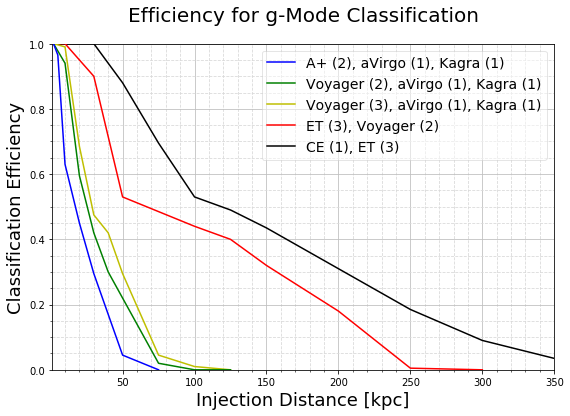
\includegraphics[width=2.75in]{figures/eff_gmode.png}
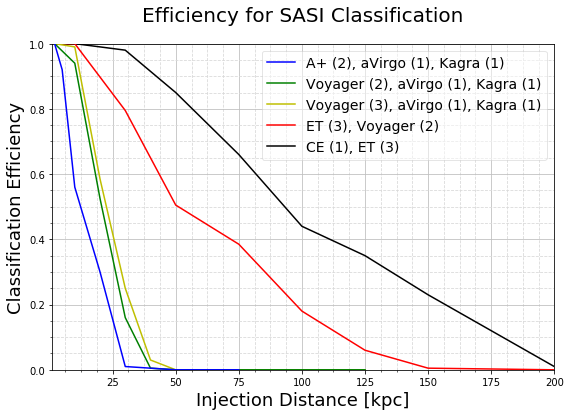
\includegraphics[width=2.75in]{figures/eff_sasi.png}
\caption{Classification efficiency for g-mode (left) and SASI (right) waveform features. Performance was better for g-mode classification in our tests, but this is also heavily dependent on the energy of the specific waveform. Overall performance was similar to that of neutrino model mechanism classification.}
\label{fig:eff_features}
\end{figure*}
\chapter{Conclusion}

GW150914 opened to the door to GW astronomy. Almost everything humanity currently knows about the universe was learned through electromagnetic observations. GWs are generated from a different force and offer an entirely new approach to studying the universe. It is not an exaggeration to compare the discovery of GW150914 to Galileo's first examination of the sky with a telescope. One or two hundred years from now, humanity's understanding of the universe may be just as fundamentally dependent on GW astronomy as it currently is on electromagnetic astronomy.

Compact binary systems will likely dominate GW observations in the near future, but new frequency bands and GW sources will become increasingly important as detectors and sensitivities improve. CCSNe represent one of the most promising and mysterious sources of GWs yet to be observed. These GWs originate in the core of a collapsing star and carry important information about processes and mechanisms that are not fully understood. An observation of a GW from a CCSN could provide clues to the nuclear equation of state and could elucidate the exact physics behind the spread of heavy metals throughout the universe. These processes, while seemingly remote and obscure, are essential to all known life.

Spectrograms offer a robust way to approach and study GW emission from a CCSN signal. The spectrogram version of SMEE presented in this dissertation does not use unreliable phase data. Instead, its statistics depend entirely on the power, frequency, and time of GW emission. This is reflected in the reduction of the number of PCs needed from those in previous studies that used the time series waveforms. The time-frequency path, inherent to a spectrogram, also allows the study and analysis of specific waveform features. This results in a robust and sensitive tool to perform the difficult task of parameter estimation of a GW signal from a CCSN. The small number of simulated waveforms is still a concern, as is the fact that most simulations are ended prematurely. As more simulations continue to be released they will be incorporated into SMEE's analysis.

The work in this dissertation contains the first study of CCSN waveforms in future detector networks. SMEE's performance in future detectors was simulated and mapped out as realistically as possible with recolored Advanced LIGO data. The results suggest that SMEE should be able to classify CCSN waveforms from well outside of the Milky Way in future detector configurations. Third generation detectors should be able to resolve the explosion mechanism and waveform features for most CCSN out to beyond the Small and Large Magellanic Clouds (50 - 60\,kpc), as well as for the dozen or so satellite galaxies in between~\cite{karachentsev2004catalog, belokurov2007cats}. A fraction of magnetorotational waveforms should be classifiable all the way out to the Andromeda galaxy (790\,kpc) in third generation detectors, while neutrino model performance falls off significantly beyond 150\,kpc. There are a total of 28 known Galaxies, mostly satellite or dwarf, within the range of 150\,kpc, and 55 within the range of 790\,kpc~\cite{karachentsev2004catalog, belokurov2007cats}. While CCSN are rare (1 - 2 per galaxy per century~\cite{1991ARA&A..29..363V, 1993A&A...273..383C, Alexeyev2002}), these results suggest that in third generation configurations a detection and accurate classification are both very plausible.

This dissertation represents the first to attempt to identify specific features associated with g-modes and SASI in detected GW signals from CCSNe. If more common features are found in future CCSN simulations, they could be incorporated into SMEE's analysis. The observation of a gravitational wave from a CCSN will be an important moment in astrophysics, and with a tool such as SMEE it will be possible to learn about the source and the relevant underlying physics of the CCSN explosion.


%%%APPENDICES
\appendix
\include{appendix1}
%%BIBILIOGRAPHY
\bibliographystyle{unsrtnat}
\bibliography{thesisbib} %%disbib.bib uses BibTex formatting.
\end{document}